\documentclass[a4paper]{article}
\usepackage[utf8]{inputenc}
\usepackage{graphicx}
\usepackage{pgfplots} % for drawing functions
\usepackage{enumerate} % for enumerating letters etc.
\usepackage{tasks} % For columned horizontal lists
\usepackage[english]{babel}
\graphicspath{ {./pics/} }
\usepackage{natbib} % For bibtex references

% For creating graphs and other diagrams
\usepackage{tikz}
\usetikzlibrary{automata, positioning, arrows, calc}
\tikzset{
  ->, % makes the edges directed
  >=stealth', % makes the arrow heads bold
  node distance=4cm, % specifies the minimum distance between two nodes. Change if necessary.
  every state/.style={thick, fill=gray!10}, % sets the properties for each ’state’ node
  initial text=$ $, % sets the text that appears on the start arrow
}

% For custom coloring
\usepackage{xcolor} % For coloring text
\definecolor{ao(english)}{rgb}{0.0, 0.5, 0.0}

% For blue click-to-go reference
\usepackage{hyperref}
	\hypersetup{
		colorlinks=true,
		linkcolor=blue,
		filecolor=magenta,      
		urlcolor=cyan,
		citecolor=ao(english)
	}
\hypersetup{linktocpage}
\usepackage{url} % For click-to-go on url-references
\usepackage{fancyhdr} % For page layout and sexy headers

\usepackage{lastpage} % For displaying the last page of the document

% For math symbols ---------------
\usepackage{amsmath}
\usepackage{amssymb}
% Left-right bracket
\newcommand{\lr}[1]{\left (#1\right)}

% Left-right square bracket
\newcommand{\lrs}[1]{\left [#1 \right]}

% Left-right curly bracket
\newcommand{\lrc}[1]{\left \{#1\right\}}

% Left-right absolute value
\newcommand{\lra}[1]{\left |#1\right|}

% Left-right upper value
\newcommand{\lru}[1]{\left \lceil#1\right\rceil}

% Scalar product
\newcommand{\vp}[2]{\left \langle #1 , #2 \right \rangle}

% The real numbers
\newcommand{\R}{\mathbb R}

% The natural numbers
\newcommand{\N}{\mathbb N}

% The integer numbers
\newcommand{\Z}{\mathbb Z}

% The rational numbers
\newcommand{\Q}{\mathbb Q}

% Expectation symbol with an optional argument
\NewDocumentCommand{\E}{o}{\mathbb E\IfValueT{#1}{\lrs{#1}}}

% Variance
\DeclareMathOperator{\V}{Var}
\NewDocumentCommand{\Var}{o}{\V\IfValueT{#1}{\lrs{#1}}}

% Indicator function with an optional argument
\NewDocumentCommand{\1}{o}{\mathds 1{\IfValueT{#1}{\lr{#1}}}}

% Probability function
\let\P\undefined
\NewDocumentCommand{\P}{o}{\mathbb P{\IfValueT{#1}{\lr{#1}}}}

% A hypothesis space
\newcommand{\HH}{\mathcal H}

% A sample space
\newcommand{\XX}{\mathcal{X}}

% A label space
\newcommand{\YY}{\mathcal{Y}}

% A nicer emptyset symbol
\let\emptyset\varnothing

% Sign operator
\DeclareMathOperator{\sign}{sign}
\newcommand{\sgn}[1]{\sign\lr{#1}}

% Argmin and argmax function
\DeclareMathOperator{\argmax}{arg\,max}
\DeclareMathOperator{\argmin}{arg\,min}

% floor operator
\newcommand{\floor}[1]{\lfloor #1 \rfloor}

% Ceil operator
\newcommand{\ceil}[1]{\lceil #1 \rceil}




% Code snippets and files ------------------
\usepackage{listings}  % For presenting code
\lstdefinestyle{mystyle}{
  language=Python,
  basicstyle=\ttfamily\footnotesize,
  backgroundcolor=\color[HTML]{F7F7F7},
  rulecolor=\color[HTML]{EEEEEE},
  identifierstyle=\color[HTML]{24292E},
  emphstyle=\color[HTML]{005CC5},
  keywordstyle=\color[HTML]{D73A49},
  commentstyle=\color[HTML]{6A737D},
  stringstyle=\color[HTML]{032F62},
  emph={@property,self,range,True,False},
  morekeywords={super,with,as,lambda},
  literate=%
    {+}{{{\color[HTML]{D73A49}+}}}1
    {-}{{{\color[HTML]{D73A49}-}}}1
    {*}{{{\color[HTML]{D73A49}*}}}1
    {/}{{{\color[HTML]{D73A49}/}}}1
    {=}{{{\color[HTML]{D73A49}=}}}1
    {/=}{{{\color[HTML]{D73A49}=}}}1,
  breakatwhitespace=false,
  breaklines=true,
  captionpos=b,
  keepspaces=true,
  numbers=left,
  showspaces=false,
  showstringspaces=false,
  showtabs=false,
  tabsize=4,
  frame=single,
}
\lstset{style=mystyle}


%%%%%%  Layout settings ------------------------------
\usepackage[a4paper, total={6in, 9in}]{geometry}
\renewcommand{\baselinestretch}{1.1} % Adjusts spacing of text
\pagestyle{fancy}
\fancyhf{}
\rhead{Magnus Raabo Andersen}
\lhead{\nouppercase \leftmark}
\rfoot{Side \thepage/ \pageref*{LastPage}}
\title{KR - Computer Networks: A Top Down Approach}
\author{Magnus Raabo Andersen}
\numberwithin{equation}{section}
\setcounter{tocdepth}{2} % Includes depth only down to subsections in table of content.

\begin{document}
\maketitle
\thispagestyle{empty}
\tableofcontents
\newpage
\setcounter{page}{1}

\section{Computer Networks and the Internet}
\subsection{What is the Internet?}
\subsubsection{What is the difference between a host and an end system? List several different types of endsystems. Is a Web server an end system? (R1)}

There is no difference, end systems are the same as hosts and are also called by that name, since they host (run) web-programs. A Web server is an end system, since it runs a web-program of sending data and receiving requests. Other examples of end systems are laptops, smartphones and tablets.

\subsubsection{Describe a protocol for two people starting and ending a conversation on a phone (R2)}

Person1 might start with ''hi'' to greet the other person and check if he is listening,. Person2 might afterwards answer with ''hi'' to confirm that he is listening. Person1 can then state this business. To conclude the conversation on person might say ''bye'' and the other person answers ''bye'' to confirm that the conversation is over. Afterwards they can both hang up.

\subsubsection{Why are standards important for protocols? (R3)}

To avoid confusion as to when to receive information and how much and when to transmit information and how much of that information can be received by the other party. Standards are generally important for creating a network of systems that can interoperate.
\subsection{The Network Edge}

\subsubsection{List four access technologies. Classify each one as home access, enterprise access, or wide-area wireless access. (R4)}

\begin{enumerate}
    \item iPhone: wide-area wireless access
    \item Stationary PC: home access
    \item Personal Laptop: home access
    \item Work LapTop: enterprise access
\end{enumerate}



\subsubsection{Is HFC transmission rate dedicated or shared among users? Are collisions possible in HFC? Why or why not? (R5)}
Hybrid fiber coax (HFC) is a combination of optical fiber and coaxial cable. The optical fiber is used for most of the length and connects neighborhood junctions, from which coaxial follows and connects to individual houses. On the downstream channel, all packets come from the same source, the head end of the fiber cable and therefore the users share the HFC bandwidth. This also means that there are no collisions.



\subsubsection{What access network technologies would be most suitable for providing internet access in rural areas? (R6)}
Rural areas are likely to be far from internet providers, which will typically lie ind the city. Therefore wireless technologies are the most suitable. As such terrestrial radio channels or satellite radio channels might provide the best solution.



\subsubsection{Dial-up modems and DSL both use the telephone line (a twisted-pair copper cable) as their transmission medium. Why then is DSL much faster than dial-up access? (R7)}

DSL is much faster than dial-up because it offers wider bandwidth (uses a wider frequency range), digital transmission (as opposed to analog, which is more susceptible to noise interference), multiple frequencies and channels, and asymmetric speed configurations. These factors allow for higher data rates compared to dial-up modems.


\subsubsection{What are some of the physical media that Ethernet can run over? (R8)}
Twisted-pair copper wire, coaxial cable, and fiber-optic cable.


\subsubsection{HFC, DSL, and FTTH are all used for residential access. For each of these access technologies, provide a range of transmission rates and comment on whether the transmission rate is shared or dedicated. (R9)}
\begin{itemize}
    \item HFC: \begin{itemize}
        \item Downstream: 40 Mbps - 1.2 Gbps
        \item Upstream: 30 Mbps - 100 Mbps
        \item Transmission rate: Shared
        \end{itemize}
    \item DSL: \begin{itemize}
        \item Downstream: 24 Mbps - 52 Mbps
        \item Upstream: 3.5 Mbps - 16 Mbps
        \item Transmission rate: Dedicated
        \end{itemize}
    \item FTTH: \begin{itemize}
        \item Downstream: Up to 100+ Gbps
        \item Upstream: Up to 100+ Mbps
        \item Transmission rate: Dedicated
        \end{itemize}
\end{itemize}


\subsubsection{Describe the different wireless technologies you use during the day and their charecteristics. If you have a choice between multiple technologies, why do you prefer one over another? (R10)}
My iPhone which i prefer for tasks that require short attention and can be performed on a small screen. A stationary PC for longer tasks that can benefit from larger and dual screens. Laptop for on-the-go tasks which require a keyboard and a larger screen than the iPhone. 
\subsection{The Network Core}

\subsubsection{Suppose there is exactly one packet switch between a sending host and a receiving host. The transmission rates between the sending host and the switch and between the switch and the receiving host are $R_1$ and $R_2$, respectively. Assuming that the switch uses store-and-forward packet switching, what is the total end-to-end delay to send a packet of length $L$? (Ignore queuing, propagation delay, and processing delay.) (R11)}

It would take $L/R_1$ time for the packet to get to the switch and then $L/R_2$ time for the packet to get to the receiving host from the switch. Since we assume no queuing or delays this gives a total end-to-end delay of $L/R_1 + L/R_2$.

\subsubsection{What advantage does a circuit-switched network have over a packet-switched network? What advantages does TDM have over FDM in a circuit-switched network? (R12)}
Circuit-switched networks does not have the same problems as packet-switched networks have regarding variable and unpredictable end-to-end delays, which makes circuit-switched networks more ideal for real-time applications such as voice and video. \\
\\
Time-division multiplexing (TDM) has the advantage over frequency-division multiplexing (FDM) that it allows for more users in a restricted bandwidth. This is because TDM allocates a time slot for each user, while FDM allocates a frequency band for each user. This means that TDM can have more users in the same bandwidth, since the users do not use the bandwidth simultaneously. TDM also has the advantage over FDM that it is easier to implement as FDM required sophisitcated analog hardware to shift signals into different frequency bands.

\subsubsection{Suppose users share a 2 Mbps link. Also suppose each user transmits continuesly at 1 Mbps when transmitting, but each user transmits only 20 percent of the time. (R13)}

\textbf{a. When circuit switching is used, how many users can be supported?}\\
When using circuit switching with multiplexing then the two users can both be serviced. This can be done with frequency-division multiplexing (FDM) where one user reserves 1 Mbps and the other user takes the other 1 Mpbs. It can also be done with time-division multiplexing (TDM) where the whole 2 Mpbs are allocated to user1 in a time interval and then switches to user2 in another interval and then back to user1 and continues this pattern. \\
\\
Since we do not know which 20 percent the users transmit we have to reserve the bandwidth in both the TDM and FDM approach. This means that no other users can join in on the bandwidth, which is the drawdown of using circuit switching. Therefore the answer is 2 users. \\
\\
\textbf{b. For the remainder of this problem, suppose packet switching is used. Why will there be essentially no queuing delay before the link if two or fewer users transmit at the same time? Why will there be queuing delay if three users transmit at the same time?} \\
Since the capacity is 2 Mbps and users transmit at 1 Mbps, then 2 users can send packets of 1 Mb per second, without queuing. This is because the rate of information sending fits exactly with the bandwidth capacity. If a third user join in, then the users try to send 3 Mbps, while the capacity is only at 2 Mpbs. This will make the packets queue up, when they are sending simultaneously. \\
\\
\textbf{c. Find the probability that a given user is transmitting.}\\
Each user transmits 20 percent of a time, meaning that at anytime there is 20 \% probability that a user is transmitting. \\
\\
\textbf{d. Suppose now there are three users. Find the probability that any given user is transmitting simultaneously. Find the fraction of time during which the queue grows.}\\
We denote $P(x_1)$ as the probability that user1 is transmitting. We know from part c that $P(x_i) = 0.2$ for any $i$. The joint distribution $P(x_1, x_2, x_3)$ can be found by
$$ P(x_1, x_2, x_3) = P(x_1)P(x_2)P(x_3)$$
as we assume independence. Inserting $P(x_i)=0.2$ for $i \in {1, 2, 3}$ we get
$$ P(x_1, x_2, x_3) = 0.2^3 = 0.008$$ 
The queue will grow as soon as 3 are transmitting at the same time. We know from the above calculation that the probability of this is 0.008. This means that on average the fraction of time, for which the queue grows, is 0.008. 


\subsubsection{Why will two ISPs at the same level of the hierarchy often peer with each other? How does an IXP earn money? (R14)}

Two ISPs at the same level of the hierarchy might find it attractive to peer with each other, since this usually happens transaction-free and can help both ISPs route traffic to more far-away costumers. An Internet Exchange Point (IXP) can earn money by being a meeting point where multiple ISPs can peer together. An IXP is a stand-alone building with a lot of switches, which the ISPs do not need to build themselves, and might like to pay for instead. 

\subsubsection{Why is a content provider considered a different Internet entity today? How does a content provider connect to other ISPs? Why? (R15)}

A content provider is considered a different Internet entity today, because they are aim to create their own network infrastructure.\\ 
\\
A content provider can connect to other ISPs by using a private peering connection, which is a direct connection between the content provider and the ISP. This is usually only done to the lower-level ISPs.\\
\\
They do this to bypass higher level ISPs and thus reduce costs. They also benefit from having greater control over how their content are provided to end users, when having their own network infrastructure. \\
\\

\subsection{Delay, Loss and Throughput in Packet-Switched Networks}

\subsubsection{Consider sending a packet from a source host to a destination host over a fixed route. List the delay components in the end-to-end delay. Which of these delays are constant and which are variable? (R16)}
\begin{itemize}
    \item \textbf{Processing delay:} The time required to examine the packet's header and determine where to direct the packet. Constant.
    \item \textbf{Queuing delay:} The time the packet spends waiting in the queue at the router. Variable as it depends on how many other packets are in the queue.
    \item \textbf{Transmission delay:} The time required to push all of the packet's bits from a switch into the link. Constant.
    \item \textbf{Propagation delay:} The time required to propagate from the beginning of the link to the next switch. Constant.
\end{itemize}



\subsubsection{Visit the Transmission Versus Propagation Delay interactive animation at the Companion Website. Among the rates, propagation delays, and packet sizes available, find a combination for which the sender finishes transmitting before the first bit of the packet reaches the receiver. Find another combination for which the first bit reaches the receiver before the sender finishes transmitting. (R17)}

The sender finishes transmitting before the first bit of the packet reaches the receiver when the length is 1000 km, the transmission rate is 512 kbs and the packet size is 100 Bytes. \\
\\
The first bit reaches the receiver before the sender finishes transmitting when the length is 10 km, the transmission rate is 512 kbs and the packet size is 1 kBytes.



\subsubsection{A user can directly connect to a server through either long-range wireless or a twisted-pair cable for transmitting a 1500-bytes file. The transmission rates of the wireless and wired media are 2 and 100 Mbps, respectively. Assume that the propagation speed in the air is $3 \times 10^8$ m/s, while the speed in the twisted-pair cable is $2 \times 10^8$ m/s. If the user is located 1 km away from the server, what is the nodal delay when using each of the two technologies? (R18)}

For the long-range wireless technology we can calculate the nodal delay by
\begin{equation*}
\begin{split}
    d_{\text{nodal}} &= d_{\text{trans}} + d_{\text{prop}} \\
    &= L/R + d/s \\
    &= \frac{1 \, 500 \times 8 \, \text{bit}}{2\, 000 \, 000 \, \text{bit/s}} + \frac{1 \, 000\, \text{m}}{3 \times 10^8 \, \text{m/s}} \\
    &= 0.006003 \, \text{s}
\end{split}
\end{equation*}
where $R$ is transmission rate, $d$ is the distance and $s$ propagation speed. We assume no processing and queuing delay since we have no information about these. \\
\\
For the twisted-pair cable we calculate the nodal delay by
\begin{equation*}
    \begin{split}
        d_{\text{nodal}} &= d_{\text{trans}} + d_{\text{prop}} \\
        &= L/R + d/s \\
        &= \frac{1 \, 500 \times 8 \, \text{bit}}{100 \, 000 \, 000 \, \text{bit/s}} + \frac{1 \, 000\, \text{m}}{2 \times 10^8 \, \text{m/s}} \\
    &= 0.000125 \, \text{s}
\end{split}
\end{equation*}



\subsubsection{Suppose Host A wants to send a large file to Host B. The path from Host A to Host B has three links, of rates $R_1 = 500 \, kbps$, $R_2 = 2 \, Mbps$, and $R_3 = 1 \, Mbps$. (R19)}

\textbf{a. Assuming no other traffic in the network, what is the throughput for the file transfer?} \\
The throughput is found by
\begin{equation*}
\begin{split}
    \text{throughput} &= \min \lr{R_1, R_2, R_3} \\
    &= 500 \, \text{kbps}
\end{split}
\end{equation*}
\\
\noindent
\textbf{b. Suppose the file is 4 million bytes. Dividing the file size by the throughput, roughly how long will it take to transfer the file to Host B?} \\
We have that 
\begin{equation*}
    \frac{4 \, 000 \, 000 \times 8 \, \text{bit}}{500 \, 000 \, \text{bit/s}} = 64 \, \text{s}
\end{equation*}
so it will take 64 seconds for the transfer. \\
\\
\textbf{c. Repeat (a) and (b), but now with $R_2$ reduced to 100 kbps.} \\
We now have that 
\begin{equation*}
    \begin{split}
        \text{throughput} &= \min \lr{R_1, R_2, R_3} \\
        &= 100 \, \text{kbps}
\end{split}
\end{equation*}
so now the time of transferring the file is
\begin{equation*}
    \frac{4 \, 000 \, 000 \times 8 \, \text{bit}}{100 \, 000 \, \text{bit/s}} = 320 \, \text{s}
\end{equation*}



\subsubsection{Suppose end system A wants to send a large file to end system B. At a very high level, describe how end system A creates packets from the file. When one of these packets arrives to a router, what information in the packet does the switch use to determine the link onto which this packet should be forwarded? Why is packet switching in the Internet analogous to driving from one city to another and asking directions along the way? (R20)}

The large file is divided into packets of smaller size and provided with a header that contains its metadata (herein the IP address of the receiver). These packets are then sent on the access link for host A. The packet then arrives at a router where the router reads the receiving IP address of the packet in the header of the packet. The router uses this information along with a forwarding table encoded in the router to determine which link the packet should be forwarded on. \\
\\
The next router has to go through the same process of reading the receiving IP address and look up in its forwarding table where to send the packet. That is why packet switching is analogous to driving from on city to another asking for direction along the way - the packets ask every router it encounters for directions on the way from host A to host B.



\subsubsection{Visit the Queuing interactive animation at the Companion Website. What is the maximum emission rate and the minimum transmission rate? With those rates, what is the traffic intensity? Run the interactive animation with these rates and determine how long it takes for packet loss to occur. Then repeat the experiment a second time and determine again how long it takes for packet loss to occur. Are the values different? Why or why not? (R21)}

The maximum emission rate is 500 packets/s and the minimum transmission rate is 350 packets/s. This makes the traffic intensity $500/350 = 1.43$. The first experiment running at these rates results in the first packet loss occurring at 9.5 mses. The second experiment running the same rates results in the first packet loss occurring at 8.8 ms. The values are different because the emission process is random and the emission rate is only an average rate of how often packets are sent on the link. 
\subsection{Protocol Layers and Their Service Models}

\subsubsection{If two end-systems are connected through multiple routers and the data-link level between them ensure reliable data delivery, is a transport protocol offering reliable data delivery between these two end-systems necessary? Why? (R22)}

Yes, the transport protocol does not only offer reliable data delivery, it also handles error and flow control.


\subsubsection{What are the five layers in the Internet protocol stack? What are the principal responsibilities of each of these layers? (R23)}
\begin{itemize}
    \item Application layer: Responsible for handling the file that is being sent and how it is divided into packets. Examples of application layer protocols are HTTP, SMTP and FTP.
    \item Transport layer: Responsible for handling packet loss and flow control. Examples of transport layer protocols are TCP and UDP.
    \item Network layer: Contains routing protocols and are responsible for handling the where the packets are sent. There is only one network layer protocol, since all Internet components must run this protocol to to agree on how to handing routing of the packets, this protocol is called IP.
    \item Link layer: Responsible for handling how the packets are sent on links. Examples of link layer protocols are Ethernet and WiFi.
    \item Physical layer: Responsible for handling how the individual bits in a packet are sent on the physical medium they travel on. The physical layer protocols depends on the medium of the link. 
\end{itemize}


\subsubsection{What do encapsulation and de-encapsulation mean? Why are they needed in a layered protocol stack? (R24)}

Encapsulation is the idea of hiding information from entities that does not need it. In relation to internet protocols this means that layers hide information from every other layer except the layer below them (which de-encapsulates the layer) because flow of certain information is needed from the layer above for it to perform its function. This is needed in a layered protocol stack to preserve the layered structure, it every layer had full information about every other layer, then the whole stack would melt together and the functionalities would no longer be divided. \\
\\
De-encapsulation is the idea of unpacking information for an entity that needs the otherwise encapsulated information. This is needed in a layered protocol stack, because if the layer below could not de-encapsulate information from the layer above, then it would not be able to perform its functionality, e.g. the transport layer could not handle packet loss and congestion if it did not the information about the packet sizes from the application layer.


\subsubsection{Which layers in the Internet protocol stack does a router process? Which layers does a link-layer switch process? Which layers does a host process? (R25)}

A router process the network, link and physical layers. A link-layer switch process the link and physical layers. A host process all layers.

\subsection{Networks Under Attack}

\subsubsection{What is self-replicating malware? (R26)}
Malware that once present on a computer can download more malware on this computer or spread itself to other computers from the infected one.


\subsubsection{Describe how a botnet can be created and how it can be used for a DDoS attack. (R27)}
A botnet is created by spreading malware on several computers, so that the hacker can control all of these computers. These can be used for a DDoS attack in the following ways:
\begin{itemize}
    \item \textbf{Bandwidth flooding}: Sending so many packets to the targeted host, that the access link of the host becomes clogged, preventing legitimate packets from reaching the host.
    \item \textbf{Connection flooding}: Sending repeated bogus requests for connection to the targeted host, causing the targeted host to stop accepting legitimate requests for connection.
\end{itemize}



\subsubsection{Suppose Alice and Bob are sending packets to each other over a computer network. Suppose Trudy positions herself in the network so that she can capture all the packets sent by Alice and send whatever she wants to Bob; she can also capture all the packets sent by Bob and send whatever she wants to Alice. List some of the malicious things Trudy can do from this position. (R28)}
Trudy can do several malicious things, with the following being only a few examples:
\begin{itemize}
    \item She can quietly intercept all packets and "sniff" on the packet being sent, if she can decrypt them. Perhaps send them to a third party.
    \item She can pretend to be Bob to Alice and pretend to be Alice to Bob, and send fake messages to both of them.
    \item She can stop the packets from reaching either Bob or Alice or both and thus prevent their communication.
    \item She can perform a combination of the above.
\end{itemize}
\subsection{History of Computer Networking and the Internet}
There are no exercises for this section.
\subsection{Problems}

\subsubsection{Design and describe an application-level protocol to be used between an automatic teller machine and a bank's centralized computer. Your protocol should allow a user's card and password to be verified, the account balance (which is maintained at the centralized computer) to be queried, and an account withdrawal to be made (that is, money disbursed to the user). Your protocol entities should be able to handle the all-too-common case in which there is not enough money in the account to cover the withdrawal. Specify your protocol by listing the messages exchanged and the action taken by the automatic teller machine or the bank's centralized computer on transmission and receipt of messages. Sketch the operation of your protocol for the case of a simple withdrawal with no errors, using a diagram similar to that in figures 1.2. Explicitly state the assumptions made by your protocol about the underlying end-to-end transport service. (P1)}

The protocol is implemented in the ATM and performs pattern-matching on the stated messages and performs the corresponding actions stated below (usually in the stated order).
\begin{enumerate}
    \item \texttt{HELLO <userid>}: Lets the ATM know that a card has been inserted and that the card belongs to the user with <userid>. The ATM them prompts for the corresponding password (PIN).
    \item \texttt{PWD <password>}: Lets the ATM know that the user has entered the password <password>. The ATM then sends <userid> and <password> to the bank's centralized computer and checks if there is a match. If not then it prompts for the password again for a for a maximum of 2 more times. If all 3 times are used then the ATM shuts down the connection and makes <userid> unable to establish a connection before they have been to the bank and reset their password.
    \item \texttt{BALANCE}: Requests the balance of the account belonging to <userid> from the bank's centralized computer. The ATM connects to the centralized computer and displays the balance for the user.
    \item \texttt{WITHDRAWAL <amount>}: Requests a withdrawal of <amount> from the account belonging to <userid> from the bank's centralized computer. The ATM connects to the centralized computer and checks if the account has enough money to cover the withdrawal. If not then the ATM displays an error message and prompts the user to enter a new amount. If the account has enough money then the ATM displays a message that the withdrawal was successful and prompts the user to take the money and the card.
    \item \texttt{BYE}: Lets the ATM know that the user has taken the card and the money and that the ATM can shut down the connection.
\end{enumerate}


\subsubsection{Equation 1.1 gives a formula for the end-to-end delay of sending one packet of length $L$ over $N$ links of transmission rate $R$. Generalize this formula for sending $P$ such packets back-to-back over the $N$ links. (P2)}
When there are $N$ links then there is $N-1$ routers between the source and destination of the $P$ packets. Assuming no delays and instantaneous propagation we have that at time $L/R$ the first packet have been sent from the source to the first router and is being transmitted to the same router, and at the same time the source is transmitting the second packet. At time 2L/R the first packet have been sent to the second router, the second packet has arrived at the first router and the source is transmitting the third packets. As described for equation 1.1. in KR, we have that this means that the first packet have arrived at the destination at $N \frac{L}{R}$. We also have that the $P$th packet is $P-1$ routers behind the first packet and that each router will take $L/R$ to traverse, meaning that the last packet arrives $(P-1) \frac{L}{R}$ after the first packet. Therefore the last packet will have arrived at time 
\begin{equation*}
    d_{\text{end-to-end}} = N \frac{L}{R} + (P-1) \frac{L}{R} = (N + P-1) \frac{L}{R}
\end{equation*}
which is by definition the end-to-end delay of sending $P$ packets back-to-back.


\subsubsection{Consider an aplication that transmits data at a steady rate (for example, the sender generates an $N$-bit unit of data every $k$ time units, where $k$ is small and fixed). Also, when such an application starts, it will continue running for a relatively long period of time. Answer the following questions, briefly justifying your answer: (P3)}

\textbf{a. Would a packet-switched network or a circuit-switched network be more appropriate for this application? Why?}\\
A circuit-switched network would be more appropriate, especially if it implemented with time-division multiplexing. This is because it allows the application to transmit over the bandwidth exactly when it needs to and only when it needs to. Since we know exactly when and how to the application needs to transmit we can allocate it to the application without any waste of bandwidth. Since the application is running for a relatively long period of time it reinforces this point since the overhead cost of setting up and tearing down connections are amortized over the lengthy period of a session. Packet-switched networks will provide more variable transmits, because it depends on the use of other users. Packet switching also have the risk of packet-loss etc. which might require packets to be retransmitted which ruins the strict transmitting policy of the application. \\
\\
\textbf{b. Suppose that a packet-switched network is used and the only traffic in this network comes from such applications as described above. Furthermore, assume that the sum of the application data rates is less than the capacities of each and every link. Is some form of congestion control needed? Why?}\\
No, if the sum of application data rates is less than the capacity of every link and since there is no bursts of transmission then we know that no packets will queue on any link. This causes no congestions and we do not need any congestion control under such conditions.



\subsubsection{Consider the circuit-switched network in Figure 1.13. Recall that there are four circuits on each link. Label the four switches A, B, C and D, going in the clockwise direction. (P4)}

\textbf{a. What is the maximum number of simultaneous connections that can be in progress at any one time in this network?}\\
Each switch have 4 links in each direction and if every switch pairs with any adjacent switch (say A-B, B-C, C-D, and D-A). Then each switch services all of its 4 links in each direction, yielding a total of 16 connections. \\
\\
\textbf{b. Suppose that all connections are between switches A and C. What is the maximum number of simultaneous connection that can be in progress?}\\
Since we only have 4 links, we use these 4 links to connect A and C, which results in a max of 4 simultaneous connections. \\
\\
\textbf{c. Suppose we want to make four connections between switches A and C, and another four connections between switches B and D. Can we route these calls through the four links to accommodate all eight connections?}\\
No. If we first make four connection between A and C, then we use all links that could otherwise go to B. If we instead first make four connections between B and D, then we use all links that could otherwise go to C. Therefore it is not possible to accommodate all eight connections. This is only possible when making connections that only use two switches as in the example given in answer of question a. 



\subsubsection{Review the car-caravan analogy in Section 1.4. Assume a propagation speed of 100 km/hour. (P5)}

The analogy assumes that the first car in a caravan to arrive at a tollbooth waits at the tollbooth for the remaining cars before servicing and passing through the tollbooth. The analogy also assumes that it takes a tollbooth 12 seconds to service a car. \\
\\
\textbf{a. Suppose the caravan travels 175 km, beginning in front of one tollbooth,
passing through a second tollbooth, and finishing just after a third tollbooth.
What is the end-to-end delay?} \\
The initial analogy assumes 10 cars. To service the cars and transmit them on the highway 3 times (transmission delay) it takes 
\begin{equation*}
    3 \cdot 10 \, \text{cars} \cdot 12 \, \text{s/cars} = 360 \, \text{s} = \frac{360 \, \text{s}}{60 \, \text{s/min}} =  6 \, min
\end{equation*}
Then to propagate them on the highway (propagation delay) it takes
\begin{equation*}
    \frac{175 \, \text{km}}{100 \, \text{km/h}} =  1.75 \, \text{h} = 1.75 \, \text{h} \cdot 60 \, \text{min/h} =  105 \, min
\end{equation*}
Here we have aggregated the two times the cars are propagated since this is equal to the sum of the two times they travel on the highway as we assume instant acceleration. Summing the delays we get that the total end-to-end-delay is $6 \, \text{min} + 105 \, \text{min} = 111 \, \text{min}$. \\
\\
\textbf{b. Repeat (a), now assuming that there are eight cars in the caravan instead
of ten.} \\
The time to propagate (propagation delay) the cars on the highway is the same as in (a) as every car accelerates instantly and at the same time. But the time to service the cars and transmit them on the highway 3 times (transmission delay) is now 
\begin{equation*}
    3 \cdot 8 \, \text{cars} \cdot 12 \, \text{s/cars} = 288 \, \text{s} = \frac{288 \, \text{s}}{60 \, \text{s/min}} =  4.8 \, min
\end{equation*}
Summing the propagation delay of 105 min and the new transmission delay of 4.8 min gives us a total end-to-end delay of $109.8 \, \text{min}$.

\subsubsection{This elementary problem begins to explore propagation delay and transmission delay, two central concepts in data networking. Consider two hosts, A and B, connected by a single link of rate $R$ bps. Suppose that the two hosts are separated by $m$ meters, and suppose the propagation speed along the link is $s$ meters/sec. Host A is to send a packet of size $L$ bits to Host B. (P6)}

\textbf{a. Express the propagation delay, $d_{\text{prop}}$, in terms of $m$ and $s$.} \\
\begin{equation*}
    d_{\text{prop}} = \frac{m}{s}
\end{equation*}
\\
\textbf{b. Determine the transmission time of the packet, $d_{\text{trans}}$, in terms of $L$ and $R$.} \\
\begin{equation*}
    d_{\text{trans}} = \frac{L}{R}
\end{equation*}
\\
\textbf{c. Ignoring processing and queuing delays, obtain an expression for the end-to-
end delay.} \\
\begin{equation*}
    d_{\text{end-to-end}} = d_{\text{trans}} + d_{\text{prop}} = \frac{L}{R} + \frac{m}{s}
\end{equation*}
\\
\textbf{d. Suppose Host A begins to transmit the packet at time $t = 0$. At time $t =
d_{\text{trans}}$, where is the last bit of the packet?} \\
The last bit has just left host A and is on the start of the link. \\
\\
\textbf{e. Suppose $d_{\text{prop}}$ is greater than $d_{\text{trans}}$. At time $t = d_{\text{trans}}$, where is the first
bit of the packet?} \\
If $d_{\text{prop}} > d_{\text{trans}}$ then it takes longer for the bits to propagate on the link than it takes for host A to transmission them on the link. In this case the first bit is still on the link at time $t = d_{\text{trans}}$. \\
\\
\textbf{f. Suppose $d_{\text{prop}}$ is less than $d_{\text{trans}}$. At time $t = d_{\text{trans}}$, where is the first
bit of the packet?} \\
In that takes it takes longer for host A to transmission the bits on the link than it takes for them to propagate on the link to host B. In that case the first bit will already have reached host B at time $t = d_{\text{trans}}$ \\
\\
\textbf{g. Suppose $s = 2.5 \cdot 10^8$, $L = 1500$ bytes, and $R = 10$ Mbps. Find the
distance $m$ so that $d_{\text{prop}}$ equals $d_{\text{trans}}$.} \\
We have that 
\begin{equation*}
\begin{split}
    d_{\text{prop}} &= d_{\text{trans}} \Longleftrightarrow \\
    \frac{m}{s} &= \frac{L}{R} \Longleftrightarrow \\
    m &= \frac{L}{R} \cdot s \Longleftrightarrow \\
    m &= \frac{1500 \cdot 8 \, \text{bits}}{10 \cdot 10^6\, \text{bits/sec}} \cdot 2.5 \cdot 10^8 \, \frac{\text{m}}{\text{sec}} = 300 \, 000 \, \text{m} = 300 \, \text{km}
\end{split}
\end{equation*}


\subsubsection{In this problem, we consider sending real-time voice from Host A to Host B over a packet-switched network (VoIP). Host A converts analog voice to a digital 64 kbps bit stream on the fly. Host A then groups the bits into 56-byte packets. There is one link between Hosts A and B; its transmission rate is 10 Mbps and its propagation delay is 10 msec. As soon as Host A gathers a packet, it sends it to Host B. As soon as Host B receives an entire packet, it converts the packet’s bits to an analog signal. How much time elapses from the time a bit is created (from the original analog signal at Host A) until the bit is decoded (as part of the analog signal at Host B)? (P7)}

First the bit is transformed to digital at host A taking $\frac{1}{64 \cdot 10^3}$ seconds. Then the bit is grouped into a packet of 56 bytes, meaning it has to wait for the remaining bits in this packet being converted to digital. The worst case of this waiting time is when the inspected bit is the first bit in the packet, which gives the worst runtime of $\frac{56 \cdot 8 - 1}{64 \cdot 10^3}$ seconds. Next the bit has to be transmitted with the packet taking $\frac{56 \cdot 8}{10 \cdot 10^6}$ seconds. Then the bit has to be propagated along with the packet taking $\frac{1}{10^3}$ seconds. We assume that the first bit to be packed by host A (as the inspected bit was in our worst-case scenario from before) is the first to be decoded into analog by host B. We also assume that host B decodes the digital signal as fast as host A encodes the analog signal to digital. This means that the time it takes host B to decode the bit is $\frac{1}{64 \cdot 10^3}$. Adding all these delays together we get 
\begin{equation*}
\begin{split}
    d &= \frac{56 \cdot 8}{64 \cdot 10^3} + \frac{56 \cdot 8}{10 \cdot 10^6} + \frac{10}{10^3} + \frac{1}{64 \cdot 10^3} \\
    &= 0.007 + 0.0000448 + 0.01 + 0.000015625 \\
    &= 0.0170604255 \, \text{s} \\
    &= 17.0604255 \, \text{ms}
\end{split}
\end{equation*}

\subsubsection{Suppose users share a 10 Mbps link. Also suppose each user requires 200 kbps when transmitting, but each user transmits only 10 percent of the time. (See the discussion of packet switching versus circuit switching in Section 1.3.) (P8)}

\textbf{a. When circuit switching is used, how many users can be supported?} \\
When circuit switching is used, bandwidth is allocated to the user whether the user transmits or not. We can therefore find the number of users that can be supported by dividing the total bandwidth by the amount required for a user.
\begin{equation*}
    \frac{10 \cdot 10^6 \, \text{bits/s}}{200 \cdot 10^3 \, \text{bits/s}} = 50
\end{equation*}
meaning that 50 users can be supported by circuit switching on this network.\\
\\
\textbf{b. For the remainder of this problem, suppose packet switching is used. Find the probability that a given user is transmitting.} \\
Since each user only transmits 10 percent of the time then the probability that a given user is transmitting must be 0.1. \\
\\
\textbf{c. Suppose there are 120 users. Find the probability that at any given time, exactly $n$ users are transmitting simultaneously. (Hint: Use the binomial distribution.)} \\
Using the binomial distribution with $p = 0.1$ (found in part b.) and $N = 120$ we get
\begin{equation*}
\begin{split}
    \P\lr{X = n} &= \binom{N}{n} p^n \lr{1 - p}^{N - n} \\
    &= \binom{120}{n} 0.1^n 0.9^{120 - n}
\end{split}
\end{equation*}
\\
\textbf{d. Find the probability that there are 51 or more users transmitting simultaneously.}
This is found by
\begin{equation*}
    \P \lr{X > 51} = 1 - \P \lr{X \leq 50}  = 1 - \sum_{n = 0}^{50} \P\lr{X = n}
\end{equation*}
since $X \in \Z^+$. Inserting the probability function found in part c we get
\begin{equation*}
\begin{split}
    \P \lr{X > 51} &= 1 - \sum_{n = 0}^{50} \binom{120}{n} 0.1^n 0.9^{120 - n} \\
    &= 3.22925 \cdot 10^{-6}
\end{split}
\end{equation*}

\subsubsection{Consider the discussion in Section 1.3 of packet switching versus circuit switching in which an example is provided with a 1 Mbps link. Users are generating data at a rate of 100 kbps when busy, but are busy generating data only with probability $p = 0.1$. Suppose that the 1 Mbps link is replaced by a 1 Gbps link. (P9)}

\textbf{a. What is $N$, the maximum number of users that can be supported simultaneously under circuit switching?} \\
This is found by 
\begin{equation*}
    \frac{1 \cdot 10^9}{100 \cdot 10^3} = 10000
\end{equation*}
\\
\textbf{b. Now consider packet switching and a user population of $M$ users. Give a formula (in terms of $p$, $M$, $N$) for the probability that more than $N$ users are sending data.} \\
We have that $X \in \Z^+$ so we can express the probability function as a binomial PDF
\begin{equation*}
\begin{split}
    \P \lr{X > N} &= \sum_{n = N + 1}^{M} \binom{M}{n} p^n (p - 1)^{M - n}
\end{split}
\end{equation*}

\subsubsection{Consider the network illustrated in Figure 1.16. Assume the two hosts on the left of the figure start transmitting packets of 1500 bytes at the same time towards Router B. Suppose the link rates between the hosts and Router A is 4-Mbps. One link has a 6-ms propagation delay and the other has a 2-ms propagation delay. Will queuing delay occur at Router A? (P10)}

From the 6-ms link we have an arrival rate of 6 ms for every packet making the traffic
\begin{equation*}
    \frac{1500 \cdot 8 \, \text{bits}}{6 \cdot 10^{-3} \, \text{s}} = 2 \text{Mb/s}
\end{equation*}
From the 2-ms link we can calculate the traffic by 
\begin{equation*}
    \frac{1500 \cdot 8 \, \text{bits}}{2 \cdot 10^{-3} \, \text{s}} = 6 \text{Mb/s}
\end{equation*}
The outgoing traffic from the link is equal to the link rate which is only 4 Mb/s. The incoming traffic is not larger than the outgoing when sent on the 6-ms delay link. However on the 2-ms delay link we have that the incoming traffic is larger than the outgoing, which means that queuing delay wil occur at router A.

\subsubsection{Consider the scenario in Problem P10 again, but now assume the links between the hosts and Router A have different rates $R_1$ and $R_2$ byte/s in addition
to different propagation delays $d_1$ and $d_2$. Assume the packet lengths for the two hosts are of $L$ bytes. For what values of the propagation delay will no queuing delay occur at Router A? (P11)}

Denote link 1 as the link with rate $R_1$ and propagation delay $d_1$ and link 2 as the link with rate $R_2$ and propagation delay $d_2$. We have that the incoming traffic for link 1 is $L/d_1$, so no queuing will occur as long as $L/d_1 < R_1$. Similarly we have that the incoming traffic for link 2 is $L/d_2$, so no queuing occurs when $L/d_2 < R_2$. We must have that both of these conditions hold, if no queuing delay is to occur at router A.


\subsubsection{Consider a client and a server connected through one router. Assume the router can start transmitting an incoming packet after receiving its first $h$ bytes instead of the whole packet. Suppose that the link rates are $R$ byte/s and that the client transmits one packet with a size of $L$ bytes to the server. What is the end-to-end delay? Assume the propagation, processing, and queuing delays are negligible. Generalize the previous result to a scenario where the client and the server are interconnected by N routers. (P12)}

We assume that $h < L$, from the words ''instead of the whole packet''. It takes $L/R$ seconds for the server to transmit the package, meaning that the router receives the packet after $L/R$ seconds. The router then transmits the first $h$ bytes of the packet which takes $h/R$ time, meaning that the client receives the first $h$ bytes after $L/R + h/R$ seconds. The router has to transmit the $h$ sized packets $L/h$ times, meaning that the total time it takes for the router to transmit the packet is $\frac{h}{R} \frac{L}{h} = \frac{L}{R}$. The end-to-end delay (i.e. time for the client to receive the whole packet) is therefore
\begin{equation*}
    d_{\text{end-to-end}} = 2 \frac{L}{R}
\end{equation*}
The router is in this scenario essentially splitting the packet up into $L/h$ sized packets. The last bit of the package is therefore arriving at the client at the same time as it would in the scenario of p.54 (router transmits whole packet) which describes equation 1.1. Therefore a client and a server connected by $N$ routers have the end-to-end delay
\begin{equation*}
    d_{\text{end-to-end}} = \lr{N + 1} \frac{L}{R}
\end{equation*}

\subsubsection{(a) Suppose N packets arrive simultaneously to a link at which no packets are currently being transmitted or queued. Each packet is of length L and the link has transmission rate R. What is the average queuing delay for the N packets? \\
(b) Now suppose that $N$ such packets arrive to the link every $LN/R$ seconds. What is the average queuing delay of a packet? (P13)}

\textbf{(a)}\\
The first packet will zero queuing time, since the queue is empty and the packet is ready to be sent right away. The second will have a queue time of $L/R$ equal to the time it takes for the first packet to be transmitted and the following third packet will have a queue time of $2L/R$ and so on. In general the $n$th packet will have a queuing delay of 
\begin{equation*}
    (n - 1) \frac{L}{R}
\end{equation*}
So the average queuing time for the N packets will be
\begin{equation*}
\begin{split}
    \overline{d}_{\text{queue}} &= \frac{1}{N} \sum_{n = 1}^N (n - 1) \frac{L}{R} \\
    &= \frac{L}{RN} \sum_{n = 1}^N (n - 1) \\
    &= \frac{L}{RN} \sum_{n = 1}^{N - 1} n \\
    &= \frac{L}{RN} \frac{N \lr{N - 1}}{2} \\
    &= \frac{L \lr{N - 1}}{2R}
\end{split}
\end{equation*}
where we have used that $\sum_{i = 1}^X i = \frac{X \lr{X + 1}}{2}$. \\
\\
\textbf{(b)}\\
It takes $LN/R$ to transmit all of the $N$ packets. This means that the buffer is empty whenever the next $N$ packets arrive. The average queuing delay over all batches of packets is therefore equal to the average queuing delay of one batch, which was found in part (a) to be $\frac{L \lr{N - 1}}{2R}$.


\subsubsection{Consider the queuing delay in a router buffer. Let $I$ denote traffic intensity; that is, $I=La/R$. Suppose that the queuing delay takes the form $IL/R (1-I)$ for $I<1$. (P14)}

\textbf{a. Provide a formula for the total delay, that is, the queuing delay plus the transmission delay.} \\
The transmission delay is defined by $L/R$ and the queuing delay is defined as $IL/R (1-I)$ for $I<1$. The total delay can therefore be expressed as
\begin{equation*}
\begin{split}
    d_{\text{end-to-end}} &= \frac{L}{R} + \frac{IL}{R \lr{1 - I}} \\
    &= \frac{L \lr{1 - I}}{R \lr{1 - I}} +  \frac{IL}{R \lr{1 - I}} \\
    &= \frac{L \lr{1 - I} + IL}{R \lr{1 - I}} \\
    &= \frac{L - LI + IL}{R \lr{1 - I}} \\
    &= \frac{L}{R \lr{1 - I}} \\
    &= \frac{L/R}{1 - I} \\
\end{split}
\end{equation*}
\\
\textbf{b. Plot the total delay as a function of $L/R$.} \\
\begin{center}
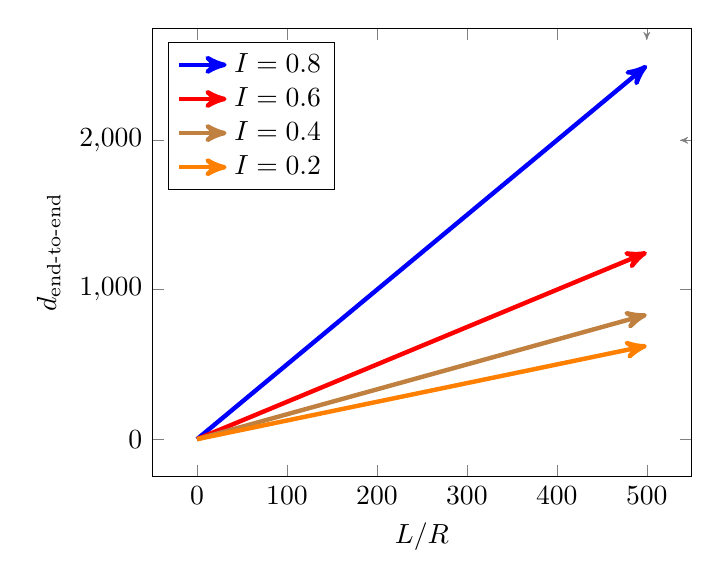
\begin{tikzpicture}
    \begin{axis}[domain=0:500, 
        samples=50, 
        legend pos=north west, 
        xlabel = $L/R$,
        ylabel = $d_{\text{end-to-end}}$]
        \addplot[blue, ultra thick] (x, x/0.2);
        \addlegendentry{$I = 0.8$}

        \addplot[red, ultra thick] (x, x/0.4);
        \addlegendentry{$I = 0.6$}

        \addplot[brown, ultra thick] (x, x/0.6);
        \addlegendentry{$I = 0.4$}

        \addplot[orange, ultra thick] (x, x/0.8);
        \addlegendentry{$I = 0.2$}
    \end{axis}
\end{tikzpicture}
\end{center}

\subsubsection{Let $a$ denote the rate of packets arriving at a link in packets/sec, and let $\mu$ denote the link's transmission rate in packets/sec. Based on the formula for the total delay (i.e., the queuing delay plus the transmission delay) derived in the previous problem, derive a formula for the total delay in terms of $a$ and $\mu$. (P15)}
Inserting $I = La/R$ and $\frac{R \, \text{bits/s}}{L \, \text{bits/packet}}= \mu \, \text{packet/s}$ into the formula for the total delay found P13 we get
\begin{equation*}
\begin{split}
    d_{\text{end-to-end}} &= \frac{L/R}{1 - I} \\
    &= \frac{L/R}{1 - La/R} \\
    &= \frac{1/\mu}{1 - a/\mu} \\
    &= \frac{1}{\mu - a}
\end{split}
\end{equation*}
which express the delay in terms of $a$ and $\mu$.

\subsubsection{Consider a router buffer preceding an outbound link. In this problem, you will use Little's formula, a famous formula from queuing theory. Let $N$ denote the average number of packets in the buffer plus the packet being transmitted. Let $a$ denote the rate of packets arriving at the link. Let $d$ denote the average total delay (i.e., the queuing delay plus the transmission delay) experienced by a packet. Little's formula is $N=a \cdot d$. Suppose that on  average, the buffer contains 100 packets, and the average packet queuing delay is 20 msec. The link's transmission rate is 100 packets/sec. Using  Little's formula, what is the average packet arrival rate, assuming there is  no packet loss? (P16)}

Isolating $a$ in Little's formula gives us
\begin{equation*}
    a = \frac{N}{d} 
\end{equation*}
we have that $N = 100$ packets/sec and $d = 0.02 \, \text{s}+ \frac{100 \, \text{packets}}{100 \, \text{packets/sec}} = 1.02$ sec. Inserting these values gives
\begin{equation*}
    a = \frac{100}{1.02} = 98.039
\end{equation*}
so the average packet arrival rate is 98.039 packets/sec.

\subsubsection{Consider the network illustrated in Figure 1.12. Would Equation 1.2 hold in such a scenario? If so, under which conditions? If not, why? (Assume $N$ is the number of links between a source and a destination in the figure.) (P17)}

The network in figure 1.12 illustrates how packets can queue up in a router when they arrive faster than they are transmitted (congestion). Equation 1.2 is $d_{\text{end-to-end}} = N \lr{d_{\text{proc}} + d_{\text{trans}} + d_{\text{prop}}}$ meaning that equation 1.2 assumes no congestion and therefore that queue delay is negligible. Equation 1.2 therefore only holds for the network in figure 1.1.2 under the condition that no congestion occurs in the network.


\subsubsection{Perform a Traceroute between source and destination on the same continent at three different hours of the day. (P18)}
First traceroute to UK at 18:30:
\begin{verbatim}
    % traceroute -I gov.uk         
    traceroute: Warning: gov.uk has multiple addresses; using 151.101.192.144
    traceroute to gov.uk (151.101.192.144), 64 hops max, 72 byte packets
     1  192.168.0.1 (192.168.0.1)  3.716 ms  2.068 ms  1.953 ms
     2  10.5.13.1 (10.5.13.1)  2.592 ms  9.268 ms  2.771 ms
     3  10.0.0.3 (10.0.0.3)  2.207 ms  2.143 ms  2.118 ms
     4  rasmusnielsenkollegiet.kbh-kua.core.fsknet.dk (130.226.217.193)  26.192 ms  
     29.797 ms  3.228 ms
     5  kbh-kua.ore.core.fsknet.dk (130.226.217.165)  2.386 ms  2.580 ms  2.723 ms
     6  dk-ore.nordu.net (109.105.102.160)  3.135 ms  2.888 ms  4.222 ms
     7  se-sthb.nordu.net (109.105.97.131)  19.990 ms  12.638 ms  13.773 ms
     8  se-bma.nordu.net (109.105.101.63)  11.224 ms  15.077 ms  11.652 ms
     9  as54113-1-100g-sk1.sthix.net (192.121.80.71)  19.065 ms  17.677 ms  19.923 ms
    10  151.101.192.144 (151.101.192.144)  19.691 ms  11.025 ms  14.791 ms
\end{verbatim}
Second traceroute to UK at 14:00:
\begin{verbatim}
    % traceroute -I gov.uk
    traceroute: Warning: gov.uk has multiple addresses; using 151.101.64.144
    traceroute to gov.uk (151.101.64.144), 64 hops max, 72 byte packets
     1  10.8.0.1 (10.8.0.1)  3.925 ms  4.567 ms  2.614 ms
     2  10.0.0.3 (10.0.0.3)  1.936 ms  2.256 ms  1.879 ms
     3  rasmusnielsenkollegiet.kbh-kua.core.fsknet.dk (130.226.217.193)  4.885 ms  
     4.215 ms  6.462 ms
     4  kbh-kua.ore.core.fsknet.dk (130.226.217.165)  3.364 ms  3.250 ms  3.097 ms
     5  dk-ore.nordu.net (109.105.102.160)  3.396 ms  3.690 ms  3.435 ms
     6  se-sthb.nordu.net (109.105.97.131)  11.425 ms  11.744 ms  11.497 ms
     7  se-kst.nordu.net (109.105.101.5)  12.650 ms  12.069 ms  11.620 ms
     8  as54113-2-100g-sk1.sthix.net (192.121.80.72)  25.837 ms  25.674 ms  25.887 ms
     9  151.101.64.144 (151.101.64.144)  11.489 ms  11.772 ms  11.753 ms
\end{verbatim}
Third traceroute to UK at 16:20:
\begin{verbatim}
    % traceroute -I gov.uk     
    traceroute: Warning: gov.uk has multiple addresses; using 151.101.0.144
    traceroute to gov.uk (151.101.0.144), 64 hops max, 72 byte packets
     1  10.8.0.1 (10.8.0.1)  9.911 ms  3.054 ms  8.821 ms
     2  10.0.0.3 (10.0.0.3)  2.316 ms  2.798 ms  2.629 ms
     3  rasmusnielsenkollegiet.kbh-kua.core.fsknet.dk (130.226.217.193)  32.219 ms  
     51.773 ms  27.735 ms
     4  kbh-kua.ore.core.fsknet.dk (130.226.217.165)  3.543 ms  6.770 ms  4.309 ms
     5  dk-ore.nordu.net (109.105.102.160)  3.133 ms  2.619 ms  3.005 ms
     6  se-sthb.nordu.net (109.105.97.131)  10.532 ms  11.647 ms  11.458 ms
     7  se-kst.nordu.net (109.105.101.1)  11.309 ms  11.988 ms  11.355 ms
     8  as54113-2-100g-sk1.sthix.net (192.121.80.72)  12.061 ms  12.802 ms  12.829 ms
     9  151.101.0.144 (151.101.0.144)  13.070 ms  12.002 ms  11.445 ms
\end{verbatim}
\textbf{a. Find the average and standard deviation of the round-trip delays at each of the three hours.} \\
Denote the vector of RTTs (round trip times) of the first traceroute as 
\begin{equation*}
\begin{split}
    \mathbf{X}_1 = &[
        3.716, 2.068, 1.953,
        2.592, 9.268, 2.771,
        2.207, 2.143, 2.118,
        26.192, 29.797, 3.228,
        2.386, 2.580, 2.723, \\
        &3.135, 2.888, 4.222,
        19.990, 12.638, 13.773,
        11.224, 15.077, 11.652,
        19.065, 17.677, 19.923,
        19.691, \\
        &11.025, 14.791
    ]
\end{split}
\end{equation*}
Then the average is $\overline{\mathbf{X}}_1 = 9.75$ and the standard deviation is $\sigma_{\mathbf{X}_1} = 8.09$. \\
\\
Denote the vector of RTTs of the second traceroute as
\begin{equation*}
\begin{split}
    \mathbf{X}_2 = &[
        3.925, 4.567, 2.614,
        1.936, 2.256, 1.879,
        4.885, 4.215, 6.462,
        3.364, 3.250, 3.097, \\
        &3.396, 3.690, 3.435,
        11.425, 11.744, 11.497,
        12.650, 12.069, 11.620,
        25.837, 25.674, 25.887,
        11.489, \\
        &11.772, 11.753
    ]
\end{split}
\end{equation*}
Then the average is $\overline{\mathbf{X}}_2 = 8.76$ and the standard deviation is $\sigma_{\mathbf{X}_2} = 7.16$. \\
\\
Denote the vector of RTTs of the third traceroute as
\begin{equation*}
\begin{split}
    \mathbf{X}_3 = &[
        9.911, 3.054, 8.821,
        2.316, 2.798, 2.629,
        32.219, 51.773, 27.735,
        3.543, 6.770, 4.309, \\
        &3.133, 2.619, 3.005,
        10.532, 11.647, 11.458,
        11.309, 11.988, 11.355,
        12.061, 12.802, 12.829,
        13.070, \\
        &12.002, 11.445
    ]
\end{split}
\end{equation*}
Then the average is $\overline{\mathbf{X}}_3 = 11.38$ and the standard deviation is $\sigma_{\mathbf{X}_3} = 10.54$. \\
\\
\textbf{b. Find the number of routers in the path at each of the three hours. Did the paths change during any of the hours?} \\
The first traceroute passes through 9 routers while the second and third passed through 9 routers. The paths must therefore have changed, which is probably because the first traceroute was performed on a different day than the day I performed the second and third traceroutes. \\
\\
\textbf{c. Try to identify the number of ISP networks that the Traceroute packets pass through from source to destination. Routers with similar names and/or similar IP addresses should be considered as part of the same ISP. In your experiments, do the largest delays occur at the peering interfaces between adjacent ISPs?} \\
Names including nordu seems to be from the same ISP. It does seem that the largest delays happen when switching between different ISP-routers. \\
\\
\textbf{d. Repeat the above for a source and destination on different continents. Compare the intra-continent and inter-continent results.} \\
First traceroute from Denmark to Japan at 18:30:
\begin{verbatim}
    % traceroute -I japan.go.jp
    traceroute: Warning: japan.go.jp has multiple addresses; using 18.173.5.29
    traceroute to japan.go.jp (18.173.5.29), 64 hops max, 72 byte packets
     1  192.168.0.1 (192.168.0.1)  3.595 ms  2.183 ms  2.009 ms
     2  10.5.13.1 (10.5.13.1)  2.750 ms  2.342 ms  2.356 ms
     3  10.0.0.3 (10.0.0.3)  2.039 ms  6.423 ms  2.322 ms
     4  rasmusnielsenkollegiet.kbh-kua.core.fsknet.dk (130.226.217.193)  4.332 ms  
     8.136 ms  7.743 ms
     5  kbh-kua.ore.core.fsknet.dk (130.226.217.165)  2.829 ms  2.856 ms  2.822 ms
     6  dk-ore.nordu.net (109.105.102.160)  3.135 ms  3.399 ms  3.399 ms
     7  dk-bal2.nordu.net (109.105.97.249)  3.499 ms  3.240 ms  3.624 ms
     8  dk-bal.nordu.net (109.105.97.48)  3.463 ms  3.461 ms  3.367 ms
     9  ndn-gw.amazon.com (109.105.98.227)  3.854 ms  3.318 ms  3.668 ms
\end{verbatim}
Second traceroute to Japan at 14:00:
\begin{verbatim}
    % traceroute -I japan.go.jp
    traceroute: Warning: japan.go.jp has multiple addresses; using 18.173.5.17
    traceroute to japan.go.jp (18.173.5.17), 64 hops max, 72 byte packets
     1  10.8.0.1 (10.8.0.1)  3.747 ms  2.488 ms  2.960 ms
     2  10.0.0.3 (10.0.0.3)  2.019 ms  2.002 ms  2.425 ms
     3  rasmusnielsenkollegiet.kbh-kua.core.fsknet.dk (130.226.217.193)  5.021 ms  
     8.438 ms  7.743 ms
     4  kbh-kua.ore.core.fsknet.dk (130.226.217.165)  2.675 ms  4.018 ms  2.508 ms
     5  dk-ore.nordu.net (109.105.102.160)  2.445 ms  2.520 ms  2.936 ms
     6  dk-bal2.nordu.net (109.105.97.249)  3.061 ms  2.909 ms  3.384 ms
     7  dk-bal.nordu.net (109.105.97.48)  3.169 ms  2.850 ms  3.438 ms
     8  ndn-gw.amazon.com (109.105.98.227)  10.382 ms  3.016 ms  3.706 ms
     9  * * *
    10  * * *
    11  * * *
    12  * * *
    13  * * *
    14  52.93.139.249 (52.93.139.249)  4.100 ms  3.657 ms  4.080 ms
    15  server-18-173-5-17.cph50.r.cloudfront.net (18.173.5.17)  3.479 ms  3.629 ms  
    3.384 ms
\end{verbatim}
Third traceroute to Japan at 16:20:
\begin{verbatim}
    % traceroute -I japan.go.jp
    traceroute: Warning: japan.go.jp has multiple addresses; using 18.173.5.104
    traceroute to japan.go.jp (18.173.5.104), 64 hops max, 72 byte packets
     1  10.8.0.1 (10.8.0.1)  4.317 ms  3.078 ms  4.614 ms
     2  10.0.0.3 (10.0.0.3)  2.441 ms  2.838 ms  2.317 ms
     3  rasmusnielsenkollegiet.kbh-kua.core.fsknet.dk (130.226.217.193)  44.191 ms  
     25.895 ms  8.237 ms
     4  kbh-kua.ore.core.fsknet.dk (130.226.217.165)  3.591 ms  3.143 ms  3.096 ms
     5  dk-ore.nordu.net (109.105.102.160)  3.236 ms  3.269 ms  2.965 ms
     6  dk-bal2.nordu.net (109.105.97.249)  3.427 ms  3.685 ms  40.914 ms
     7  dk-bal.nordu.net (109.105.97.48)  3.428 ms  3.624 ms  3.357 ms
     8  ndn-gw.amazon.com (109.105.98.227)  3.666 ms  3.820 ms  3.416 ms
     9  * * *
    10  * * *
    11  * * *
    12  * * *
    13  * * *
    14  52.93.139.249 (52.93.139.249)  6.761 ms  3.785 ms  3.631 ms
    15  server-18-173-5-104.cph50.r.cloudfront.net (18.173.5.104)  4.741 ms  3.155 ms  
    2.952 ms
\end{verbatim}
Denote the vector of RTTs of the first japanese traceroute by
\begin{equation*}
\begin{split}
    \mathbf{Z}_1 = &[
        3.595, 2.183, 2.009,
        2.750, 2.342, 2.356,
        2.039, 6.423, 2.322,
        4.332, 8.136, 7.743,
        2.829, 2.856, 2.822, \\
        &3.135, 3.399, 3.399,
        3.499, 3.240, 3.624,
        3.463, 3.461, 3.367,
        3.854, 3.318, 3.668
    ]
\end{split}
\end{equation*}
Then the average RTT of the first traceroute is $\overline{Z}_1 = 3.56$ and the standard deviation is $\sigma_{Z_1} = 1.50$. \\
\\
Denote the vector of RTTs of the second japanese traceroute by
\begin{equation*}
\begin{split}
    \mathbf{Z}_2 = &[
        3.747, 2.488, 2.960,
        2.019, 2.002, 2.425,
        5.021, 8.438, 7.743,
        2.675, 4.018, 2.508,
        2.445, 2.520, 2.936, \\
        &3.061, 2.909, 3.384,
        3.169, 2.850, 3.438,
        10.382, 3.016, 3.706,
        4.100, 3.657, 4.080,
        3.479, 3.629, 3.384
    ]
\end{split}
\end{equation*}
Then the average RTT of the second traceroute is $\overline{Z}_2 = 3.74$ and the standard deviation is $\sigma_{Z_2} = 1.86$. \\
\\
Denote the vector of RTTs of the third japanese traceroute by
\begin{equation*}
\begin{split}
    \mathbf{Z}_3 = &[
        4.317, 3.078, 4.614,
        2.441, 2.838, 2.317,
        44.191, 25.895, 8.237,
        3.591, 3.143, 3.096,
        3.236, 3.269, 2.965, \\
        &3.427, 3.685, 40.914,
        3.428, 3.624, 3.357,
        3.666, 3.820, 3.416,
        6.761, 3.785, 3.631,
        4.741, 3.155, 2.952
    ]
\end{split}
\end{equation*}
Then the average RTT of the third traceroute is $\overline{Z}_3 = 7.05$ and the standard deviation is $\sigma_{Z_3} = 10.36$. \\
\\
The path of first japanese traceroute consists of 9 routers while (not counting the timeouts) the second the third traceroute had a path if 10 paths. The difference in routers might be explained by the fact that the second on third traceroute was performed on one day and the first traceroute on another. \\
\\
On the traceroutes to japan we see that amazon is used as an ISP to go to Japan. It is also the transition from this ISP to the next that causes the biggest delays (and a couple of timeouts).

\subsubsection{Metcalfe's law states the value of a computer network is proportional to the square of the number of connected users of the system. Let $n$ denote the number of users in a computer network. Assuming each user sends one message to each of the other users, how many messages will be sent? Does your answer support Metcalfe's law? (P19)}

If $n$ users each send a message to every other $n - 1$ users then the messages sent wil be $n(n- 1) = n^2 - n$. This means that the number of messages sent is proportional to $n$ the users in the network, which supports Metcalfe's law, if the value of a computer network is proportional to the messages sent.


\subsubsection{Consider the throughput example corresponding to Figure 1.20(b). Now suppose that there are $M$ client-server pairs rather than 10. Denote $R_s$, $R_c$, and $R$ for the rates of the server links, client links, and network link. Assume all other links have abundant capacity and that there is no other traffic in the network besides the traffic generated by the $M$ client-server pairs. Derive a general expression for throughput in terms of $R_s$, $R_c$, $R$, and $M$. (P20)}

The transmission rate is $R_s$ on the server-side, $R_c$ on the client side where each server and client have their own link. The transmission rate is $R/M$ in the shared network core link. The smallest of theses rates will act as the bottleneck for the throughput and therefore the throughput can be expressed as
\begin{equation*}
    \text{throughput} = \min \lr{R_s, R_c, \frac{R}{M}}
\end{equation*}



\subsubsection{Assume a client and a server can connect through either network (a) or (b) in Figure 1.19. Assume that $R_i=(R_c + R_s)/i$, for $i=1, 2, \dots, N$. In what case will network (a) have a higher throughput than network (b)? (P21)}

In both networks the throughput is bounded by the transmission rate of the bottleneck link. In network (a) this means that the throughput is $\min \lr{R_c, R_s}$ and in network (b) it means that throughput is $\min \lr{R_1, R_2, \dots, R_N} = \min \lr{\frac{R_c + R_s}{1}, \frac{R_c + R_s}{2}, \dots, \frac{R_c + R_s}{N}} = \frac{R_c + R_s}{N}$. It therefore follows that network (a) will have a higher throughput than network (b) when
\begin{equation*}
    \min \lr{R_c, R_s} > \frac{R_c + R_s}{N}
\end{equation*}



\subsubsection{Consider Figure 1.19(b). Suppose that each link between the server and the client has a packet loss probability $p$, and the packet loss probabilities for these links are independent. What is the probability that a packet (sent by the server) is successfully received by the receiver? If a packet is lost in the path from the server to the client, then the server will re-transmit the packet. On average, how many times will the server re-transmit the packet in order for the client to successfully receive the packet? (P22)}

The probability that a packet sent by the server is successfully received by the receiver can be calculated by 
\begin{equation*}
    P_s = (1 - p)^N
\end{equation*}
\\
The average times the server re-transmit the packet can be found by using that the number of transmissions needed for the receiver to obtain the packet follows a geometric distribution with success probability $p_s$. We therefore have that the average transmits is given by $1/p_s$, and therefore the average re-transmits must be given by
\begin{equation*}
    \E \lr{\text{Re-transmits}} = \frac{1}{p_s - 1} 
\end{equation*}



\subsubsection{Consider Figure 1.19(a). Assume that we know the bottleneck link along the path from the server to the client is the first link with rate $R_s$ bits/sec. Suppose we send a pair of packets back to back from the server to the client, and there is no other traffic on this path. Assume each packet of size $L$ bits, and both links have the same propagation delay $d_{\text{prop}}$. (P23)}

\textbf{a. What is the packet inter-arrival time at the destination? That is, how much time elapses from when the last bit of the first packet arrives until the last bit of the second packet arrives?} \\
We must have that the propagation delay only parallel shifts the first and second packet, such that the distance between them is constant. On the other hand the transmission delay will cause the second packet to queue while the first packet is being transmitted at the bottleneck link which is along the first link with rate $R_s$. Here we have that the second packet will be transmitted after the first packet has spent $\frac{R_s}{L}$ being sent. Therefore the packet inter-arrival time must be
\begin{equation*}
    \frac{R_s}{L}
\end{equation*}
\\
\textbf{b. Now assume that the second link is the bottleneck link (i.e., $R_c < R_s$). Is it possible that the second packet queues at the input queue of the second link? Explain. Now suppose that the server sends the second packet $T$ seconds after sending the first packet. How large must $T$ be to ensure no queuing before the second link? Explain} \\
Yes, it is possible that the second packet queues at the input queue of the second link. This is the case if the first packet is still being transmitted from the second link when the second packet arrives. The time it takes for the first packet to have been transmitted by the second link is; the time it takes to transmit it from the server $L/R_s$ plus the time it takes to propagate to the second link $d_{\text{prop}}$ plus the time it takes for the second link to transmit it $L/R_c$. The time it takes for the second packet to arrive at the second link is the time it is waiting for the first packet to be transmitted $L/R_s$ plus the time it takes for the second packet to be transmitted $L/R_s$ plus the time it takes to propagate the second packet to the second link $d_{\text{prop}}$. We therefore have that the second packet queues at the second link when
\begin{equation*}
\begin{split}
    2\frac{L}{R_s} + d_{\text{prop}} &< \frac{L}{R_s} + d_{\text{prop}} + \frac{L}{R_c} \Longleftrightarrow \\
    \frac{L}{R_s}  &<  \frac{L}{R_c} \Longleftrightarrow \\
    \frac{1}{R_s} &< \frac{1}{R_c} \Longleftrightarrow \\
    R_c &< R_s
\end{split}
\end{equation*}
where the lefthandside is the time it takes the second packet to reach the second link and the right hand side is the time it takes the first packet to be transmitted from the second link. We see that the results is exactly the case where the second link is the bottleneck, we therefore know that the second packet will queue in that case. \\
\\
Now that the server sends the second packet $T$ seconds after the first packet, we have from the above equation that the second packet will not queue when
\begin{equation*}
\begin{split}
    R_c + T & \geq R_s \Longleftrightarrow \\
    T &\geq R_s - R_c
\end{split}
\end{equation*}
so the waiting time $T$ must be at least the positive difference in transmission rate.


\subsubsection{Consider a user who needs to transmit 1.5 gigabytes of data to a server. The user lives in a village where only dial-up access is available. As an alternative, a bus collects data from users in rural areas and transfer them to the Internet through a 1 Gbps link once it gets back to the city. The bus visits the village once a day and stops in front of the user's house just long enough to receive the data. The bus has a 100 Mbps WiFi connection. Suppose the average speed of the bus is 60 km/h and that the distance between the village and the city is 150 km. What is the fastest way the user can transfer the data to the server? (P24)}

The end-to-end delay of using the bus can be expressed as
\begin{equation*}
    d_\text{end-to-end} = d_\text{bus-transmit} + d_\text{bus-prop} + d_\text{link-transmit}
\end{equation*}
here we have that $d_\text{bus-transmit} = \frac{1.5 \cdot 10^9 \, \text{bit}}{100 \cdot 10^6 \, \text{bit/s}} = 15 \, \text{s}$, $d_\text{bus-prop} = \frac{150 \cdot 10^3 \, \text{m}}{60/3.6 \, \text{m/s}} = 9000 \, \text{s}$, and $d_\text{link-transmit} = \frac{1.5 \cdot 10^9 \, \text{bit}}{1 \cdot 10^9 \, \text{bit/s}} = 1.5 \, \text{s}$. Inserting these values we get
\begin{equation*}
    d_\text{end-to-end} = 15 + 9000 + 1.5 = 9016.5 \, \text{s}
\end{equation*}
What is fastest depends on the rate of the dial-up access, it this takes less than $9016.5$ seconds then dial-up is fastest otherwise the bus is fastest (not counting that waiting for the bus can take up to a day).



\subsubsection{Suppose two hosts, A and B, are separated by 20,000 kilometers and are connected by a direct link of $R = 5$ Mbps. Suppose the propagation speed over the link is $2.5 \cdot 10^8$ meters/sec. (P25)}

\textbf{a. Calculate the bandwidth-delay product, $R \cdot d_\text{prop}.$} \\
\begin{equation*}
    R \cdot d_\text{prop} = 5 \cdot 10^6 \, \text{bits/s} \cdot \frac{20 \, 000 \cdot 10^3 \, \text{m}}{2.5 \cdot 10^8 \, \text{m/s}} = 4 \cdot 10^5 \, \text{bits}
\end{equation*}
\\
\textbf{b. Consider sending a file of 800,000 bits from Host A to Host B. Suppose the file is sent continuously as one large message. What is the maximum number of bits that will be in the link at any given time?} \\
The time from the first bit is transmitted on the link (and the second bit is being transmitted) to the time host B receives this first bit must be $d_\text{prop}$. We must now find how many bits we maximum could have been transmitted on the link at this time (thus not accounting for whether the last bit left host A at an earlier time). This can be calculated by the transmission rate $R$ times the time spent transmitting $d_\text{prop}$, which is the bandwidth-delay product, $R \cdot d_\text{prop}.$ calculated in part a. We can therefore at maximum transmit $4 \cdot 10^5$ bits on the link at the same time, since this number is smaller then the file of $8 \cdot 10^5$ bits, it means that the file was not finished being transferred before the link was filled with bits. The maximum amount of bits that will be in the link at any time is therefore $4 \cdot 10^5$ bits. \\
\\
\textbf{c. Provide an interpretation of the bandwidth-delay product.} \\
The bandwidth-delay product is the amount of bits that can be on the link when transmitting continuously. \\
\\
\textbf{d. What is the width (in meters) of a bit in the link? Is it longer than a football field?} \\
Assuming the link is filled with bits, then we have $4 \cdot 10^5$ bits on a length of $20 \, 000 \cdot 10^3$ meters, meaning that each bit is
\begin{equation*}
    \frac{20 \, 000 \cdot 10^3 \, \text{m}}{4 \cdot 10^5  \, \text{bits}} = 50 \, \text{m/bit}
\end{equation*}
According to wikipedia\footnote{\url{https://en.wikipedia.org/wiki/American_football_field}} an american football field is 48.8 m wide and 91.44 m long, so a bit is longer then the but not longer than the length of a football field. \\
\\
\textbf{e. Derive a general expression for the width of a bit in terms of the propagation speed $s$, the transmission rate $R$, and the length of the link $m$.} \\
From part a. we had that the bandwidth-delay product was calculated by $R \frac{m}{s}$, and from part d. we calculated the width of a bit by dividing $m$ by the bandwidth-delay product. We can therefore express the width of a bit by
\begin{equation*}
    \text{width of bit} = \frac{m}{R \frac{m}{s}} = \frac{ms}{Rm} = \frac{s}{R}
\end{equation*}
which is the propagation speed divided by the transmission rate. 



\subsubsection{Consider problem P25 but now with a link of R = 1 Gbps. (P26)}

\textbf{a. Calculate the bandwidth-delay product, $R \cdot d_{\text{prop}}$.} \\
\begin{equation*}
    R \cdot d_\text{prop} = 1 \cdot 10^9 \, \text{bits/s} \cdot \frac{20 \, 000 \cdot 10^3 \, \text{m}}{2.5 \cdot 10^8 \, \text{m/s}} = 8 \cdot 10^7 \, \text{bits}
\end{equation*}
\\
\textbf{b. Consider sending a file of 800,000 bits from Host A to Host B. Suppose the file is sent continuously as one big message. What is the maximum number of bits that will be in the link at any given time?} \\
As before this is equal to the bandwidth-delay product unless this is larger than the file in which case the file can not stretch along the entire link. In this case we have that the file is $8 \cdot 10^5$ bits, which is lower than the bandwidth-delay product. The faster transmit-speed in relation to propagation speed, compared to P25, now results in the file being transmitted on the link so fast that the every bit of the file can be on the link, i.e. the last bit is transmitted on the link before the first bit is received. Therefore the maximum number of bits on the link will be equal to the file size of $8 \cdot 10^5$ bits. \\
\\
\textbf{c. What is the width (in meters) of a bit in the link?} \\
Using the formula from P25 part e. we have
\begin{equation*}
    \text{width of bit} = \frac{s}{R} = \frac{2.5 \cdot 10^8 \, \text{m/s}}{ 1 \cdot 10^9 \, \text{bits/s}} =  0.25 \, \text{m/bit}
\end{equation*}



\subsubsection{Consider the scenario illustrated in Figure 1.19(a). Assume $R_s$ is 20 Mbps, $R_c$ is 10 Mbps, and the server is continuously sending traffic to the client. Also assume the router between the server and the client can buffer at most four messages. After how many messages sent by the server will packet loss starts occurring at the router? (P27)}

Since $R_s/R_c = 2$ then the server transmits messages to the router twice as fast as the router transmits these messages to the client link. This means that each time the server sends 2 messages the messages in the routers buffer is incremented by 1. Therefore after the server has sent 8 messages the buffer holds 4 messages and is therefore full, meaning that the 9th message sent from the server will be lost as it arrives at the buffer before the router can transmit a message from the buffer. The answer is therefore that the server can send 8 messages before packet loss occurs at the router.



\subsubsection{Generalize the result obtained in Problem P27 for the case where the router can buffer m messages. (P28)}
Since we still have $R_s/R_c = 2$ the server transmits messages twice as fast as the router can transmit them to the client. So again we have that for every 2 messages the buffer holds 1 more message. The buffer is therefore full after the server has sent $2m$ messages and packet loss will start occurring.


\subsubsection{Suppose there is a 10 Mbps microwave link between a geostationary satellite and its base station on Earth. Every minute the satellite takes a digital photo and sends it to the base station. Assume a propagation speed of $2.4 \cdot 10^8$ meters/sec. (P29)}

\textbf{a. What is the propagation delay of the link?} \\
\begin{equation*}
    d_{\text{prop}} = \frac{m}{s} = \frac{36 \, 000 \cdot 10^3 \, \text{m}}{2.4 \cdot 10^8 \, \text{m/s}} = 0.15 \, \text{s}
\end{equation*}
where $m$ is the distance between the satellite and earth in meters (which is provided in the solution to be 36,000 kilometers away from earth surface) and $s$ is the propagation speed. \\
\\
\textbf{b. What is the bandwidth-delay product, $R \cdot d_{\text{prop}}$?} \\
\begin{equation*}
    R \cdot d_{\text{prop}} = 10 \cdot 10^6 \, \text{bits/s} \cdot 0.15 \, \text{s} = 15 \cdot 10^5 \, \text{bits}
\end{equation*}
\\
\textbf{c. Let $x$ denote the size of the photo. What is the minimum value of $x$ for the microwave link to be continuously transmitting?} \\
For the microwave link to be continuously transmitting the file must the large enough to still be transmitting after 1 minute where a new file is generated. The time to transmit $x$ bits can be expressed as $x/R$ so mathematically we must have
\begin{equation*}
\begin{split}
    \frac{x}{10 \cdot 10^6 \, \text{bits/s}} &\geq 60 \, \text{s} \Leftrightarrow \\
    x &\geq 10 \cdot 10^6 \, \text{bits/s} \cdot 60 \, \text{s} \Leftrightarrow \\
    x &\geq 6 \cdot 10^8 \, \text{bits}
\end{split}
\end{equation*}
So the file must be at least 600 Mbits for the microwave link to be continuously transmitting.


\subsubsection{Consider the airline travel analogy in our discussion of layering in Section 1.5, and the addition of headers to protocol data units as they flow down the protocol stack. Is there an equivalent notion of header information that is added to passengers and baggage as they move down the airline protocol stack? (P30)}

Let the passenger and his baggage be the analogy of the data unit to be transferred. We then have that the passenger purchase tickets to enable the transfer. This adds a tag to the ticket and the baggage. The baggage tag is propagated and used by the baggage layer to couple the passenger and his baggage and so that the baggage is transported with the passenger and can reunite with him on arrival. The ticket tag is propagated to the gates layer and used for identifying where the passenger should be directed for transport. Showing up at the gate in turn is required by the runway take-off for initiating transport, which ends in the Airplane routing that takes care of the transport of passenger and baggage. 




\subsubsection{In modern packet-switched networks, including the Internet, the source host segments long, application-layer messages (for example, an image or a music file) into smaller packets and sends the packets into the network. The receiver then reassembles the packets back into the original message. We refer to this process as message segmentation. Figure 1.27 illustrates the end-to-end transport of a message with and without message segmentation. Consider a message that is $10^6$ bits long that is to be sent from source to destination in Figure 1.27. Suppose each link in the figure is 5 Mbps. Ignore propagation, queuing, and processing delays. (P31)}

\textbf{a. Consider sending the message from source to destination without message segmentation. How long does it take to move the message from the sourcehost to the first packet switch? Keeping in mind that each switch uses store-and-forward packet switching, what is the total time to move the message from source host to destination host?} \\
The time to move to the first packet switch is
\begin{equation*}
    d_\text{1st switch} = \frac{L}{R} = \frac{10^6 \, \text{bits}}{5 \cdot 10^6 \, \text{bits/s}} = 0.2 \, \text{s}
\end{equation*}
We have that there are two packet switches and that these use store-and-forward packet switching, meaning that they only transmit a packet once they have received every bit of the packet (in contrary to continuously transmitting the packet as soon as it receives the first bit). We must therefore have that the total time to move the message from source to host is: the time to the 1st packet switch plus the time to the 2nd packet switch plus the time to the host, which is
\begin{equation*}
    d_\text{end-to-end} = 3\frac{L}{R} = 3 \cdot 0.2 \, \text{s} = 0.6 \, \text{s}
\end{equation*}
\\
\textbf{b. Now suppose that the message is segmented into 100 packets, with each packet being 10,000 bits long. How long does it take to move the first packet from source host to the first switch? When the first packet is being sent from the first switch to the second switch, the second packet is being sent from the source host to the first switch. At what time will the second packet be fully received at the first switch?} \\
The time it takes the first packet to reach the first switch can be found by
\begin{equation*}
    d_\text{1st packet to 1st switch} = \frac{L}{R} = \frac{10^4 \, \text{bits}}{5 \cdot 10^6 \, \text{bits/s}} = 0.002 \, \text{s}
\end{equation*}
The time (started at beginning of the transmission of the first bit) it takes for the second packet to be fully received at the first switch is: the time it takes for the first packet to be received by the 1st switch $d_\text{1st packet to 1st switch}$ plus the time it takes for the second packet to be transmitted from the host $L/R$ (since we neglect propagation delay). This is calculated by
\begin{equation*}
     d_\text{2nd packet to 1st switch} = d_\text{1st packet to 1st switch} + \frac{L}{R} = 2 \frac{L}{R} = 2 \cdot 0.002 \, \text{s} = 0.004 \, \text{s}
\end{equation*}
\\
\textbf{c. How long does it take to move the file from source host to destination host when message segmentation is used? Compare this result with your answer in part (a) and comment.} \\
We have that the file is segmented into 100 packets, so the last packet will start to be transmitted from the source when 99 packets have been transmitted, which will be at time $99 \frac{L}{R}$. This packet will have been transmitted to the 1st switch $L/R$ after, and will be transmitted from the 1st switch and arrived at the second switch $L/R$ seconds after this, and finally arrived at the client after $L/R$ more seconds. This means that the last packet is received by the client at time 
\begin{equation*}
     d_\text{end-to-end} = (99 + 3) \frac{L}{R} = 102 \cdot 0.002 \, \text{s} =  0.204 \, \text{s}
\end{equation*}
It therefore takes 0.204 seconds to move the file from source to client when using message segmentation, which is faster than the 0.6 seconds (as found in part a.) that it takes to send the entire file in a single packet. \\
\\
\textbf{d. In addition to reducing delay, what are reasons to use message segmentation?} \\
Message segmentation divides traffic along the links and switches contrary to sending the whole file as a large packet. This helps avoid congestion and packet loss, since a limited buffer might be able to hold a few smaller segmented messages but not the large single-file message. Another reason is in the case where bit-errors are not tolerated for the application and therefore requires resending the faulty packet. In this case message segmentation means that we only have to retransmit a small packet instead of the whole file. \\
\\
\textbf{e. Discuss the drawbacks of message segmentation.} \\
Packets have to be reassembled at the destination. Since header size are the same for all packets, we have to send a bigger total of header-bits when using message segmentation rather than sending one large packet with a single header.


\subsubsection{Consider Problem P31 and assume that the propagation delay is 250 ms. Recalculate the total time needed to transfer the source data with and without segmentation. Is segmentation more beneficial or less if there is propagation delay? (P32)}

It is assumed that the propagation delay stated is for every link and not for the entire distance from source to client. Initially assume no segmentation. Then transmitting and propagating the packet to the 1st switch takes $\frac{L}{R} + d_\text{prop}$ seconds. This is the time it also takes from the 1st switch to the 2nd switch and is identical for every link. We therefore have
\begin{equation*}
     d_\text{end-to-end} = 3 \lr{\frac{L}{R} + d_\text{prop}} = 3 \lr{  \frac{10^6 \, \text{bits}}{5 \cdot 10^6 \, \text{bits/s}} + 250 \cdot 10^{-3} \, \text{s}} = 1.35 \, \text{s}
\end{equation*}
We now assume message segmentation. We have that the last (100th) packet is being transmitted on the link after $99 L_\text{seg}/R$. As stated above every link requires transmitting and propagating the packet, so the total time it takes the packet to be transmitted to and propagated along the 3 links must be $3 \lr{\frac{L_\text{seg}}{R} + d_\text{prop}}$. The last packet will therefore have arrived at the client at time
\begin{equation*}
\begin{split}
     d_\text{end-to-end}^{\text{seg}} &= 3 \lr{\frac{L_\text{seg}}{R} + d_\text{prop}} + 99 \frac{L_\text{seg}}{R} \\
     &= 3 \lr{  \frac{10^4 \, \text{bits}}{5 \cdot 10^6 \, \text{bits/s}} + 250 \cdot 10^{-3} \, \text{s}} + 99  \frac{10^4 \, \text{bits}}{5 \cdot 10^6 \, \text{bits/s}} \\
     &= 0.954 \, \text{s}
\end{split}
\end{equation*}
Here we have not checked for queuing since this will not occur as propagation and transmission times are equal for all packets, which means they are parallel-shifted along the links, and therefore we will always have that a switch receives a packet just as it has finished transmitting the previous packet. \\
\\
We see that even with propagation delay we still have a shorter delay when using message segmentation. But not as significant as without propagation delay in P31. In that case not using message segmentation resulted in a delay larger by a factor of approximately 3, and now with propagation that factor is approximately 1.4.


\subsubsection{Consider sending a large file of $F$ bits from Host A to Host B. There are three links (and two switches) between A and B, and the links are uncongested (that is, no queuing delays). Host A segments the file into segments of $S$ bits each and adds 80 bits of header to each segment, forming packets of $L = 80 + S$ bits. Each link has a transmission rate of $R$ bps. Find the value of $S$ that minimizes the delay of moving the file from Host A to Host B. Disregard propagation delay. (P33)}
The time it takes for each packet to go from source to client can be expressed as taking $L/R$ seconds for each link (as it only needs to be transmitted on each link). We have that the last $F/S$th packet will begin transmitting at time $ \lr{\frac{F}{S} - 1} \frac{L}{R}$. We will therefore have that the last packet has arrived at time
\begin{equation*}
\begin{split}
    d_\text{end-to-end} &= \lr{\frac{F}{S} - 1} \frac{L}{R} + 3 \frac{L}{R} \\
    &= \lr{\frac{F}{S} + 2} \frac{L}{R} \\
    &= \lr{\frac{F}{S} + 2} \frac{80 + S}{R}
\end{split}
\end{equation*}
For finding the value of $S$ that minimizes this function we take the derivative with respect to $S$ (on Wolfram Alpha)
\begin{equation*}
    \frac{\partial \, d_\text{end-to-end}}{\partial \, S} = \frac{2 \lr{S^2 - 40F}}{R S^2}
\end{equation*}
Setting the derivate equal to 0 and solving for $S$ (also on Wolfram Alpha) we get the solutions $S = \pm \sqrt{40 F}$ and since we can only use the positive solution (as number of packets must be $\N^+$), we have that the lowest possible delay comes from segmenting the file into packets of $S = \sqrt{40 F}$ bits.

\subsubsection{Early versions of TCP combined functions for both forwarding and reliable delivery. How are these TCP variants located in the ISO/OSI protocol stack? Why were forwarding functions later separated from TCP? What were the consequences? (P34)}

These TCP variant are located in both the application and transport layer of the OSI protocol stack. Its lies in the application layer as this layer handles reliable delivery, which is dictated by the application (does the application tolerate bit-errors or not etc.). It also lies in the transport layer as it handles forwarding, which is the responsibility of this layer. \\
\\
As the internet evolved and networking requirements became more diverse, it was realized that combining forwarding and reliable delivery in the same protocol had certain drawbacks. The separation of forwarding functions from TCP led to the development of IP (Internet Protocol) and the creation of the TCP/IP protocol suite. The reasons for separating forwarding functions from TCP were primarily driven by the need for scalability, flexibility, and efficiency in handling different types of data traffic and network topologies:
\begin{itemize}
    \item \textbf{Scalability}: With forwarding functions handled separately by IP, routers and switches can focus on efficient data packet forwarding without the overhead of maintaining connection state information, as done in TCP. This separation allows routers to scale better in large networks with a large number of connections.
    \item \textbf{Flexibility}: By separating the forwarding function, networks can accommodate various communication models, such as connectionless protocols like UDP (User Datagram Protocol). Not all applications require the level of reliability provided by TCP, and some may prefer the reduced overhead and lower latency of connectionless communication.
    \item \textbf{Efficiency}: TCP's connection-oriented approach comes with additional overhead due to the establishment and maintenance of connections. For certain types of data, like real-time streaming or voice communication, a connectionless approach may be more efficient.
\end{itemize}







\section{Application Layer}
\subsection{Principles of Network Applications}


\subsubsection{List five nonproprietary Internet applications and the application-layer protocols
that they use. (R1)}
\begin{enumerate}
    \item Websites: HTTP or HTTPS
    \item File-transfer: FTP
    \item Remote Login: Telnet
    \item e-mail: SMTP
    \item BitTorrent: BitTorrent Protocol
\end{enumerate}


\subsubsection{What is the difference between network architecture and application architecture? (R2)}
The network architecture is the five-layer Internet architecture discussed in chapter 1, which defines how everything regarding end-to-end communication works over the Internet. Application architecture, on the other hand, defines how the application is structured over the various end systems and is designed by the application developer.


\subsubsection{For a communication session between a pair of processes, which process is the client and which is the server? (R3)}
The process that \textit{initiates} the communication is labeled as the client, while the process that waits to be contacted is called the server.


\subsubsection{Why are the terms client and server still used in peer-to-peer applications? (R4)}
To simplify the description of the communication. Even though the communicating entities can change from being the server and the client, this change of roles only happens when a new connection is established. In a P2P network the receiver of the file is the client while the sender of the file is the server. 


\subsubsection{What information is used by a process running on one host to identify a process running on another host? (R5)}
the IP address of the destination host and the port number of the socket in the destination process.


\subsubsection{What is the role of HTTP in a network application? What other components are needed to complete a Web application? (R6)}
HTTP defines the format and sequence of messages exchanged between browser and Web server. Other component like a server that stores the files available from the web-application or manages billing etc., might be other important components of a Web application.


\subsubsection{Referring to Figure 2.4, we see that none of the applications listed in Figure 2.4 requires both no data loss and timing. Can you conceive of an application that requires no data loss and that is also highly time-sensitive? (R7)}
High-frequency trading software, since it only profits from small variations in a time series, that it must evaluate and trade on in real-time, thus requiring both timing and no data loss.


\subsubsection{List the four broad classes of services that a transport protocol can provide. For each of the service classes, indicate if either UDP or TCP (or both) provides such a service. (R8)}

\begin{itemize}
    \item \textbf{Reliable data transfer}: TCP provides a reliable byte-stream but UDP does not.
    \item \textbf{Throughput}: Neither TCP Nor UDP guarantees that a certain value of throughput is maintained.
    \item \textbf{Timing}: Neither TCP nor UDP guarantees that packets/bytes arrive with a specific timing.
    \item \textbf{Security}: Neither TCP nor UDP provides any security measures like encrypting the message.
\end{itemize}

\subsubsection{Recall that TCP can be enhanced with TLS to provide process-to-process security services, including encryption. Does TLS operate at the transport layer or the application layer? If the application developer wants TCP to be enhanced with TLS, what does the developer have to do? (R9)}

TLS is an enhancement of TCP, but with the enhancements being implemented in the application layer, as it offers encryption of the application itself. For a developer to enhance TCP with TLS he will have to include TLS code in both the client and server side of the application, as both sides needs to be able to encrypt and decrypt the application.





















\subsection{The Web and HTTP}


\subsubsection{What is meant by a handshaking protocol? (R10)}
It is a protocol that defines how a client and a serves initiates a connection before transporting the application.


\subsubsection{How can websites keep track of users? Do they always need to use cookies? (R12)}
Most websites use cookies to keep track of users. Cookies work by having the server send a cookie header line in the response message the first time a user visits the website. This cookie header contains the identification number of the user. The client then response with its usual request along with a cookie header containing the same identification number (to accept the identification by this number). The ID number is then inserted in a cookie file that is kept both on the clients end system is managed by The browser and on the websites back-end database. The website can then perform cookie-specific actions, i.e. user-specific actions, and reply to the client accordingly. On subsequent visits the the website the browser will initially pass a cookie header to the server, and thereby identify the user to the server. \\
\\
No, a website have other means than cookies to track its users, some of which are
\begin{itemize}
    \item \textbf{Session IDs}: IDs that are stored as parameters in the URLs or hidden form fields, for identifying users temporarily while they navigate the website
    \item \textbf{Local storage}: HTML5 permits websites to store data locally on a user's device.
    \item \textbf{Server-side tracking}: Storing user-related information on the server associating it with the user's session or account.
    \item \textbf{Browser fingerprinting}: Collecting information about a user's browser and device configurations.
    \item \textbf{OAuth tokens or JSON Web Tokens}: Tokens that are securely generated and exchanged between client and server.
    \item \textbf{Device recognition}: Websites can store characteristics of user's devices such as IP addresses, user agent, screen resolution.
\end{itemize}


\subsubsection{Describe how Web caching can reduce the delay in receiving a requested object. Will Web caching reduce the delay for all objects requested by a user or for only some of the objects? Why? (R13)}
Web caching can reduce delay by being placed a number of links closer to the client than the server while storing the most recently requested data from the server. There is therefore a chance that the data only needs to be send the distance from the client to the web cache, if the web cache happens to be storing the requested data. \\
\\
No the web cache does not necessarily  reduce delay for all objects requested. If the web cache is not currently storing the requested objects, then it needs to request it from the server, before sending it to the client. This means that an additional connection needs to be established and the delay is therefore larger (by the time it takes to establish a connection) in this case than if the client was connecting directly to the server without the web cache acting a middleman. \\
\\
On the other hand it is possible that Web caching reduce delay for a user even when the requested object is not currently stored in the web cache, since the existence of a web cache likely reduce traffic on the link to the server (since other user's who have their requested objects stored in the web cache will not use this link).


\subsubsection{Telnet into a Web server and send a multiline request message. Include in the request message the \texttt{If-modified-since}: header line to force a response message with the \texttt{304 Not Modified} status code. (R14)}
\begin{verbatim}
GET /~remzi/OSTEP/ HTTP/1.1
Host: pages.cs.wisc.edu
If-modified-since: Fri, 18 Aug 2023 22:30:00 GMT
\end{verbatim}


\subsubsection{What is the HOL blocking issue in HTTP/1.1? How does HTTP/2 attempt to solve it? (R18)}

Head of Line (HOL) blocking is when a very large object, in terms of bytes, is on the top of a page before many small objects. This causes the small objects to wait for the large one to be sent. This makes the user-perceived delay to be much larger than if the smaller object could be loaded fast before the large object. HTTP/1.1 attempts to solve this problem by opening multiple TCP connections and sending the object in parallel. However this causes two new problems; one is having a larger number of sockets that needs to be opened and maintained at servers, the second is that this ''cheats'' TCP congestion controls in bottlenecks since these allocate $1/n$ths of the bandwidth to each TCP connection, when there are $n$ total connection over the link, thus grabbing a larger portion than intended. \\
\\
HTTP/2 attempts to solve the HOL blocking issue without creating a need for multiple parallel TCP connections for transporting a single Web page. This is done by breaking each message into small frames and interleaving the request and response message on the same TCP connection. This is done by collecting the portion of the large objects with the smaller objects in frames. These frames are then sent sequentially, and reassembled into the original message at the server-side. This causes the smaller objects to be sent alog with the larger objects and thus faster, than if they had to wait for the larger objects to be sent first. This reduce user-perceived delay without needing to maintain multiple TCP connections.
\subsection{Electronic Mail in the Internet}

\subsubsection{What does a stateless protocol mean? Is IMAP stateless? What about SMTP? (R11)}

A stateless protocol is one that does not require the server to maintain information about the user. IMAP is used to communicate with mailservers and is not a stateless protocol, since everything it transfers is maintained in a mail server (emails, folders flags, etc.) SMTP on the other hand is stateless as it functions as a protocol used for pushing email from on mail server to another. SMTP treats each transfer as an independent transaction and does not require any information maintained about previous messages sent.



\subsubsection{Are there any constraints on the format of the HTTP body? What about the email message body sent with SMTP? How can arbitrary data be transmitted over SMTP? (R15)}

Yes, the format of the HTTP body is states in the header of the HTTP message, so the receiver knows what to expect and how to interpret the body. Such formatting requirements could be the content-type (e.g. XML or JSON), encoding and length. For SMTP certain formatting requirements must be satisfied in the body; only plaintext and MIME-encoded content (used for pictures and attachments etc., which i interpret is what is meant by arbitrary data).



\subsubsection{Suppose Alice, with a Web-based e-mail account (such as Hotmail or Gmail), sends a message to Bob, who accesses his mail from his mail server using IMAP. Discuss how the message gets from Alice's host to Bob's host. Be sure to list the series of application-layer protocols that are used to move the message between the two hosts. (R16)}

Alice's host sends the message to her mail server over HTTP. Alice's mailserver then sends the message to Bob's mailserver over SMTP. Bob then transfers the message from his mail server to his host over HTTP. 

\subsubsection{Print out the header of an e-mail message you have recently received. How many \texttt{Received}: header lines are there? Analyze each of the header lines in the message. (R17)}

I received 5 header lines. 
\begin{verbatim}
Received: by 2002:a54:3405:0:b0:229:db56:e5cb with SMTP id l5csp1352389ecq;
    Mon, 21 Aug 2023 03:07:57 -0700 (PDT)
\end{verbatim}
\begin{verbatim}
X-Received: by 2002:a05:6e02:973:b0:34b:aebd:a512 with SMTP id
    q19-20020a056e02097300b0034baebda512mr7254811ilt.14.1692612477236;
\end{verbatim}
\begin{verbatim}
Received: from o1.email.toggl.com (o1.email.toggl.com. [167.89.11.255])
    by mx.google.com with ESMTPS id j2-20020a63e742000000b00563dde13952si6802499pgk.
    720.2023.08.21.03.07.56
    for <magnusraabo@gmail.com>
    (version=TLS1_3 cipher=TLS_AES_128_GCM_SHA256 bits=128/128);
    Mon, 21 Aug 2023 03:07:57 -0700 (PDT)
\end{verbatim}
\begin{verbatim}
Received-SPF: pass (google.com: domain of bounces+99121-6f98-magnusraabo=gmail.com@em4938.
    track.toggl.com designates 167.89.11.255 as permitted sender) client-ip=167.89.11.255;
\end{verbatim}
\begin{verbatim}
Received: by filterdrecv-7bd4cff9b4-bvd8j with SMTP id
    filterdrecv-7bd4cff9b4-bvd8j-1-64E3377C-55
    2023-08-21 10:07:56.541415726 +0000 UTC m=+8850582.239888199
\end{verbatim}
\begin{verbatim}
Received: from smtp-relay-75546b4bf5-7jcs4.localdomain (unknown) by geopod-ismtpd-15 (SG) 
    with ESMTP id o0jxJsdySjqk0c81t6dxIA for <magnusraabo@gmail.com>; Mon, 21 Aug 2023 10:07:56.419 +0000 (UTC)
\end{verbatim}
The header line above indicates the id of the SMTP server that sends and stores the email in my SMTP server.
\subsection{DNS - the Internet's Directory Service}


\subsubsection{Why are MX records needed? Would it not be enough to use a CNAME record? (Assume the email client looks up email addresses through a Type A query and that the target host only runs an email server.) (R19)}

MX records are needed when an organization wants their mail server to have the same alias as one of their other servers. If the target host only runs an email server, then MX is not needed and it would indeed be enough to use a CNAME record.


\subsubsection{What is the difference between recursive and iterative DNS queries? (R20)}

A recursive query is when a DNS server asks another DNS server to obtain a mapping on its behalf (by quering other DNS servers). An iterative DNS query is when a DNS server queries for a mapping by itself, without asking intermediary DNS servers to query on its behalf.

\subsection{Peer-to-Peer File Distribution}


\subsubsection{Under what circumstances is file downloading through P2P much faster than through a centralized client-server approach? Justify your answer using Equation 2.2. (R21)}

We have that P2P downloading is faster than using centralized client-server when the delay using P2P, $D_{P2P}$, is lower than the delay when using centralized client-server, $D_{cs}$. Inserting equations 2.1 and 2.2 we have that
\begin{equation*}
\begin{split}
      D_{cs} &> D_{P2P} \Longleftrightarrow \\
      \max \frac{NF}{u_s}, \frac{F}{d_\text{min}} &> D_{P2P} \geq \max \lrc{\frac{F}{u_s}, \frac{F}{d_\text{min}}, \frac{NF}{u_s + \sum_{i = 1}^{N} u_i}}
\end{split}
\end{equation*}
Since $D_{P2P}$ is only lower bounded we cannot say when P2P is faster than CS, unless we assume the set of circumstances where each peer can redistribute a bit as soon as it receives it, so that there is a redistribution scheme that achieves the lower bound(kumar2006) (which is also equation 2.3 in the book). In that case we have that P2P is faster when
\begin{equation*}
\begin{split}
      D_{cs} &> D_{P2P} \Longleftrightarrow \\
      \max \lrc{\frac{NF}{u_s}, \frac{F}{d_\text{min}}} &> \max \lrc{\frac{F}{u_s}, \frac{F}{d_\text{min}}, \frac{NF}{u_s + \sum_{i = 1}^{N} u_i}}
\end{split}
\end{equation*}
which we see is the case when $N > 1$ and $\sum_{i = 1}^{N} u_i > 0$ and $\max \lrc{\frac{F}{u_s}, \frac{F}{d_\text{min}}, \frac{NF}{u_s + \sum_{i = 1}^{N} u_i}} \neq \frac{F}{d_\text{min}}$. In other words P2P is faster than a centralized client-server when the network is larger than 1 person and the peers in the network contribute to the upload stream and the lowest download rate of the peers is not a bottleneck causing the largest delay.


\subsubsection{Consider a new peer Alice that joins BitTorrent without possessing any chunks. Without any chunks, she cannot become a top-four uploader for any of the other peers, since she has nothing to upload. How then will Alice get her first chunk? (R22)}

Every 30 seconds a peers picks a neighbor at random and sends it chunks, which is called making that peer optimistically unchoked. Alice can therefore receive her first chunk by being optimistically unchoked by random chance, and afterwards she has the opportunity to become a top-four uploader.


\subsubsection{Assume a BitTorrent tracker suddenly becomes unavailable. What are its consequences? Can files still be downloaded? (R23)}

It has the consequences that new peers trying to join the network will experience delay since they rely on the tracker to initially discover peers. If you are already connected to a list of peers, then you can still download and upload files. BitTorrent is designed to be decentralized so the absence of a tracker does not prevent data transfer between peers that have already established a connection.


\subsection{Video Streaming and Content Distribution Networks}


\subsubsection{CDNs typically adopt one of two different server placement philosophies. Name and briefly describe them. (R24)}
\begin{itemize}
    \item \textbf{Enter Deep:} Deploy server clusters in access ISPs all over the world, with the aim of getting close to end users. This improves user-perceived delay and throughput by reducing the number of links between the user and the CDN server, which sends the content.
    \item \textbf{Bring Home:} Bringing the ISPs home by building large clusters at a smaller number of sites. Instead of getting inside the access ISPs, the CDNs using this strategy place their clusters at IXPs (Internet Exchange Points). This results in lower maintenance and management overhead than enter deep, but possible at an expense of higher delays and lower throughput to end users.
\end{itemize}


\subsubsection{Besides network-related considerations such as delay, loss, and bandwidth performance, there are other important factors that go into designing a CDN server selection strategy. What are they? (R25)}

ISP delivery cost. Clusters might be chosen so that content is distributed on the cheapest route of links.
\subsection{Socket Programming: Creating Network Applications}



\subsubsection{In Section 2.7, the UDP server described needed only one socket, whereas the TCP server needed two sockets. Why? If the TCP server were to support $n$ simultaneous connections, each from a different client host, how many sockets would the TCP server need? (R26)}

The UDP protocol does not specify a welcoming socket, so for the UDP server all incoming data from different clients enters through one socket. TCP on the other hand has a specified welcoming socket, which handles all client initiation with the server before a new socket is created to handle each connection. Therefore handling $n$ simultaneous connection would require $n + 1$ sockets for the TCP server, $n$ sockets for each connection and 1 welcoming socket.



\subsubsection{For the client-server application over TCP described in Section 2.7, why must the server program be executed before the client program? For the client-server application over UDP, why may the client program be executed before the server program? (R27)}

The TCP client starts by trying to connect to the TCP server, so if the server if not executed first, then the client will simply fail to connect. On the contrary the UDP client does not attempt to connect immediately but first construct the packet and the sends it on a link. So the UDP server does not need to be executed before the client, and only needs to be executed before the packet arrives at the server socket, so that it is not lost.
\subsection{Problems}



\subsubsection{True or false? (P1)}

\textbf{a. A user requests a Web page that consists of some text and three images. For this page, the client will send one request message and receive four response messages.}\\
False, if the text and images can fit in a packet, it will only receive a single message.\\
\\
\textbf{b. Two distinct Web pages (for example, \texttt{www.mit.edu/research.html} \\ and \texttt{www.mit.edu/students.html}) can be sent over the same persistent connection.} \\
True, there is no reason two webpages can not be received on the same connection. \\
\\
\textbf{c. With nonpersistent connections between browser and origin server, it is possible for a single TCP segment to carry two distinct HTTP request messages.} \\
False, if the connections are nonpersistent then sending each message requires setting up a TCP segment. Therefore sending two messages on nonpersistent connections requires two TCP segments.\\
\\
\textbf{d. The \texttt{Date}: header in the HTTP response message indicates when the object in the response was last modified.} \\
False, it indicates when the HTTP response message was created or last modified. \texttt{Last-Modified:} indicates when the object was created or last modified. \\
\\
\textbf{e. HTTP response messages never have an empty message body.} \\
False, e.g. when sending GET-requests the message body is empty.



\subsubsection{SMS, iMessage, Wechat, and WhatsApp are all smartphone real-time messaging systems. After doing some research on the Internet, for each of these systems write one paragraph about the protocols they use. Then write a paragraph explaining how they differ. (P2)}

\begin{itemize}
    \item \textbf{SMS}: Stateless protocol that works by sending messages to a short message service center (SMSC), which provides a ''store and forward'' mechanism where messages are queued if the recipient is unreachable. Message delivery is ''best effort'', meaning that there is no guaranteed that messages are delivered. 
    \item \textbf{IMessage}: Protocol based on the Apple Push Notification service (APNs), which is a proprietary, binary protocol. It sets up a Keep-Alive connection with Apple servers, where messages are TLS-encrypted and stored on the servers for 30 days.
    \item \textbf{Wechat}: Protocol called MMTLS based on Transport Layer Security (TLS). Accounts registered with chinese phone numbers have their data stored in China for surveillance and censoring politically sensitive subjects. Other accounts have data stored in the Netherlands with stricter privacy policy.
    \item \textbf{WhatsApp}: Freeware protocol based on a customized version of the open standard Extensible Messaging and Presence Protocol (XMPP). Uses end-to-end encryption.
\end{itemize}
The services differ in regards to privacy, since Whatsapp and IMessage are encryption, SMS is not and Wechat is surveyed and censored. SMS uses the text messaging plan we purchase from our wireless carrier while the others uses Wi-Fi.


\subsubsection{Assume you open a browser and enter \texttt{http://yourbusiness.com/about.html} in the address bar. What happens until the webpage is displayed? Provide details about the protocol(s) used and a high-level description of the messages exchanged. (P3)}

First a DNS-lookup is performed to get the IP address of the URL. When the IP and socket number has been received then for UDP the request message is simply sent to the socket, while for TCP the connection is first established at this welcoming socket and then the request is sent to the connection socket. Since the request message is in the form of HTTP a GET token will be inserted in the header of the HTTP message. \\
\\
When the request is received the server will send a HTTP message via the established socket with ''200 OK'' in the header line (assuming it found the html-file) and the html-file will be sent in the body of the message. The client will receive the message via its established socket and the browser will unpack the html-file for the user to see.


\subsubsection{Consider the following string of ASCII characters that were captured by Wireshark when the browser sent an HTTP GET message (i.e., this is the actual content of an HTTP GET message). The characters \texttt{<cr><lf>} are carriage return and line-feed characters (that is, the italized character string \texttt{<cr>} in the text below represents the single carriage-return character that was contained at that point in the HTTP header). Answer the following questions, indicating where in the HTTP GET message below you find the answer. (P4)}

\begin{verbatim}
GET /cs453/index.html HTTP/1.1<cr><lf>Host: gai
a.cs.umass.edu<cr><lf>User-Agent: Mozilla/5.0 (
Windows;U; Windows NT 5.1; en-US; rv:1.7.2) Gec
ko/20040804 Netscape/7.2 (ax) <cr><lf>Accept:ex
t/xml, application/xml, application/xhtml+xml, text
/html;q=0.9, text/plain;q=0.8,image/png,*/*;q=0.5
<cr><lf>Accept-Language: en-us,en;q=0.5<cr><lf>Accept-
Encoding: zip,deflate<cr><lf>Accept-Charset: ISO
-8859-1,utf-8;q=0.7,*;q=0.7<cr><lf>Keep-Alive: 300<cr>
<lf>Connection:keep-alive<cr><lf><cr><lf>
\end{verbatim}
\noindent
\textbf{a. What is the URL of the document requested by the browser?} \\
\texttt{http://gaia.cs.umass.edu/cs453/index.html} \\
\\
\textbf{b. What version of HTTP is the browser running?} \\
HTTP/1.1 \\
\\
\textbf{c. Does the browser request a non-persistent or a persistent connection?} \\
From \texttt{Connection:keep-alive} we can see that the browser requests a persistent connection. \\
\\
\textbf{d. What is the IP address of the host on which the browser is running?} \\
Not included in message, can be acquired by the IP datagram that carried the TCP segment that carried the HTTP GET request. \\
\\
\textbf{e. What type of browser initiates this message? Why is the browser type needed in an HTTP request message?} \\
Mozilla/5.0, which can be seen by \texttt{User-Agent: Mozilla/5.0}. The browser type is required information for the server for it to be able to send different version of the same object to different browsers.


\subsubsection{The text below shows the reply sent from the server in response to the HTTP GET message in the question above. Answer the following questions, indicating where in the message below you find the answer. (P5)}

\begin{verbatim}
HTTP/1.1 200 OK<cr><lf>Date: Tue, 07 Mar 2008
12:39:45GMT<cr><lf>Server: Apache/2.0.52 (Fedora)
<cr><lf>Last-Modified: Sat, 10 Dec2005 18:27:46
GMT<cr><lf>ETag: ”526c3-f22-a88a4c80”<cr><lf>Accept-
Ranges: bytes<cr><lf>Content-Length: 3874<cr><lf>
Keep-Alive: timeout=max=100<cr><lf>Connection:
Keep-Alive<cr><lf>Content-Type: text/html; charset=
ISO-8859-1<cr><lf><cr><lf><!doctype html public ”-
//w3c//dtd html 4.0transitional//en”><lf><html><lf>
<head><lf> <meta http-equiv=”Content-Type”
content=”text/html; charset=iso-8859-1”><lf> <meta
name=”GENERATOR” content=”Mozilla/4.79 [en] (Windows NT
5.0; U) Netscape]”><lf> <title>CMPSCI 453 / 591 /
NTU-ST550ASpring 2005 homepage</title><lf></head><lf>
<much more document text following here (not shown)>
\end{verbatim}
\noindent
\textbf{a. Was the server able to successfully find the document or not? What time was the document reply provided?} \\
The document was found as indicated by the OK message and status code 200. The time can be seen in the first line: 07/03/2008 12:39:45 GMT. \\
\\
\textbf{b. When was the document last modified?} \\
Sat, 10/12/2005 18:27:46. \\
\\
\textbf{c. How many bytes are there in the document being returned?} \\
Indicated by \texttt{Ranges:} we see that it is 3874 bytes. \\
\\
\textbf{d. What are the first 5 bytes of the document being returned? Did the server agree to a persistent connection?} \\
The first 5 bytes received are \texttt{<!doc}. We see from \texttt{Connection:Keep-Alive} that it is a persistent connection.


\subsubsection{Obtain the HTTP/1.1 specification (RFC 2616). Answer the following
questions: (P6)}

\textbf{a. Explain the mechanism used for signaling between the client and server to indicate that a persistent connection is being closed. Can the client, the server, or both signal the close of a connection?} \\
According to RFC 2616 8.1.2.1 a persistent connection is closed by putting the close token ''close'' in the header, which can be done by both the server and the client. \\
\\
\textbf{b. What encryption services are provided by HTTP?} \\
HTTP does not provide encryption, this is provided by HTTPS. \\
\\
\textbf{c. Can a client open three or more simultaneous connections with a given server?} \\
RFC 2616 8.1.4 states ''Clients that use persistent connections SHOULD limit the number of
simultaneous connections that they maintain to a given server.'' which indicates that a client is not limited to any number of simultaneous connections. \\
\\
\textbf{d. Either a server or a client may close a transport connection between them if either one detects the connection has been idle for some time. Is it possible that one side starts closing a connection while the other side is transmitting data via this connection? Explain.} \\
RFC 2616 8.1.4 states that '' A client, server, or proxy MAY close the transport connection at any time. For example, a client might have started to send a new request at the same time that the server has decided to close the "idle" connection. From the server's point of view, the connection is being closed while it was idle, but from the client's point of view, a request is in progress.''. This means that the answer is yes, one side can start closing the connection while the other side is transmitting data.


\subsubsection{Suppose within your Web browser, you click on a link to obtain a Web page. The IP address for the associated URL is not cached in your local host, so a DNS lookup is necessary to obtain the IP address. Suppose that $n$ DNS servers are visited before your host receives the IP address from DNS; the successive visits incur an RTT of $RTT_1, \dots , RTT_n$. Further suppose that the Web page associated with the link contains exactly one object, consisting of a large amount of HTML text. Let $RTT_0$ denote the RTT between the local host and the server containing the object. Assuming transmission duration of $0.002 \cdot RTT_0$ of the object, how much time elapses from when the client clicks on the link until the client receives the object? (P7)}
Time to get the IP is $\sum_{i = 1}^{n} RTT_n$. Once the IP is known it takes $RTT_0$ to set up the TCP connection, $RTT_0$ to request the object and $0.002 \cdot RTT_0$ to receive the object. The total response time is therefore
\begin{equation*}
    2.002 \cdot RTT_0 + \sum_{i = 1}^{n} RTT_n
\end{equation*}

\subsubsection{Consider Problem P7 again and assume $RTT_0 = RTT_1 = RTT_2 = \dots = RTT_n = RTT$, Furthermore, assume a new HTML file, small enough to have negligible transmission time, which references nine equally small objects on the same server. How much time elapses with: (P8)}

\textbf{a. non-persistent HTTP with no parallel TCP connections?} \\
This connection will require a handshake for each request of an object, meaning that it takes $2 \cdot RTT$ for each object. The total response time is therefore $18 \cdot RTT$. \\
\\
\textbf{b. non-persistent HTTP with the browser configured for 6 parallel connections?} \\
This connection also requires a handshake for each request of an object but since 6 messages can be sent in parallel it takes $2 \cdot RTT$ for the first 6 objects and $2 \cdot RTT$ for the last 3 objects. The total response time is therefore $4 \cdot RTT$. \\
\\
\textbf{c. persistent HTTP?} \\
A singe persistent connection without pipelining needs only transmit a single handshake followed by the requests for each of the objects. The total response time is therefore $10 \cdot RTT$.


\subsubsection{Consider Figure 2.12, for which there is an institutional network connected to the Internet. Moreover, assume the access link has been upgraded to 54 Mbps, and the institutional LAN is upgraded to 10 Gbps. Suppose that the average object size is 1,600,000 bits and that the average request rate from the institution's browsers to the origin servers is 24 requests per second. Also suppose that the amount of time it takes from when the router on the Internet side of the access link forwards an HTTP request until it receives the response is three seconds on average (see Section 2.2.5 in \cite{kr}). Model the total average response time as the sum of the average access delay (that is, the delay from Internet router to institution router) and the average Internet delay. For the average access delay, use $\Delta /(1 - \Delta \beta)$, where $\Delta$ is the average time required to send an object over the access link and $\beta$ is the arrival rate of objects to the access link. (P9)}

\textbf{a. Find the total average response time.} \\
Since we are asked to find the total average response time as the sum
\begin{equation*}
    \overline{d}_\text{total} = \overline{d}_\text{access} + \overline{d}_\text{internet}
\end{equation*}
(with no LAN delay) we are looking from the point of the institutional router and we can neglect the LAN-connection from the institutional router to the requesting browsers (perhaps because the LAN Rate is high enough for the delay to be negligible. From $\overline{d}_\text{total if hit}$ calculated in b. we see that the additional delay would be 0.0002). \\
\\
We have been given that $\overline{d}_\text{internet} = 3 \, \text{s}$. So we only need to calculate the access delay. The time to transmit an object of size $L$ over a link with rate $R$ is $L/R$. Letting $\overline{L}$ be the average size of the object we have that
\begin{equation*}
\begin{split}
    \Delta &= \frac{\overline{L}}{R} \\
    &= \frac{1 \, 600 \, 000 \, \text{bits/object}}{54 \cdot 10^6 \, \text{bits/s}} \\
    &= 0.0296 \, \text{s/object}
\end{split} 
\end{equation*}
and
\begin{equation*}
    \beta = 24 \, \text{objects/s}
\end{equation*}
So using the provided formula we have that the average access delay must be 
\begin{equation*}
\begin{split}
    \overline{d}_\text{access} &= \frac{\Delta}{1 - \Delta \beta} \\
    &= \frac{0.0296 \, \text{s/object}}{1 - \lr{ \lr{0.0296 \, \text{s/object}} \cdot \lr{ 24 \, \text{objects/s}}}} \\
    &= 0.1022 \, \text{s/object}
\end{split}
\end{equation*}
The total average response time is therefore
\begin{equation*}
\begin{split}
    \overline{d}_\text{total} &= \overline{d}_\text{access} + \overline{d}_\text{internet} \\
    &= 0.1022 \, \text{s/object} + 3 \, \text{s/object} \\
    &= 3.1022 \, \text{s/object}
\end{split}
\end{equation*}
\textbf{b. Now suppose a cache is installed in the institutional LAN. Suppose the miss rate is 0.3. Find the total response time.} \\
If a request is satisfied by the cache, then the object only has to travel by LAN, and we have that the total average response time is 
\begin{equation*}
\begin{split}
    \overline{d}_\text{total if hit} &= \frac{1 \, 600 \, 000 \, \text{bits/object}}{10 \cdot 10^9 \, \text{bits/s}} \\
    &= 0.0002 \, \text{s/object}
\end{split}
\end{equation*}
If a request is not satisfied by the cache, then we have the total delay will be the sum of, the time it took to get response from the cache, the time it takes for the cache to get the object from the access router, and the time it takes for the access router to get the object from the internet. We can express this as 
\begin{equation*}
    \overline{d}_\text{total if miss} = \overline{d}_\text{LAN} + \overline{d}_\text{access} + \overline{d}_\text{internet}
\end{equation*}
where we already know that $\overline{d}_\text{LAN} = 0.0002$ and $\overline{d}_\text{internet} = 3$. \\
\\
To find $\overline{d}_\text{access}$ we need to calculate it using the new arrival rate since the traffic has changed as on average only 30\% of all requests are not satisfied by the cache and needs to go through the access and internet links.
\begin{equation*}
\begin{split}
    \beta &= 0.3 \cdot 24 \, \text{objects/s} \\
    &= 7.2000 \, \text{objects/s}
\end{split}
\end{equation*}
Meaning that we now have
\begin{equation*}
    \begin{split}
        \overline{d}_\text{access} &= \frac{\Delta}{1 - \Delta \beta} \\
        &= \frac{0.0296 \, \text{s/object}}{1 - \lr{ \lr{0.0296 \, \text{s/object}} \cdot \lr{ 7.2 \, \text{objects/s}}}} \\
        &= 0.0376 \, \text{s/object}
\end{split}
\end{equation*}
Inserting the values we get
\begin{equation*}
\begin{split}
    \overline{d}_\text{total if miss} &= \overline{d}_\text{LAN} + \overline{d}_\text{access} + \overline{d}_\text{internet} \\
    &= 0.0002 \, \text{s/object} + 0.0376 \, \text{s/object} + 3 \, \text{s/object} \\
    &= 3.0378 \, \text{s/object}
\end{split}
\end{equation*}
Since we have that on average the cache misses 30\% of the time we have that the average total response time can be calculated by
\begin{equation*}
\begin{split}
    \overline{d}_\text{total} &= 0.3 \cdot \overline{d}_\text{total if miss}  + \lr{1 - 0.3} \overline{d}_\text{total if hit} \\
    &= 0.91148 \, \text{s/object}
\end{split}
\end{equation*}


\subsubsection{Consider a 30-meter link, over which a sender can transmit at a rate of 300 bits/sec in both directions. Suppose that packets containing data are 100,000 bits long, and packets containing only control (e.g., ACK or handshaking) are 200 bits long. Assume that $N$ parallel connections each get $1/N$ of the link bandwidth. Now, consider the HTTP protocol and suppose that each downloaded object is 100 Kbits long, and that the initial downloaded object contains 10 referenced objects from the same sender. Would parallel downloads via parallel instances of non-persistent HTTP make sense in this case? Now consider persistent HTTP. Do you expect significant gains over the non-persistent case? Justify and explain your answer. (P10)}

Since the non-persistent parallel instances share the bandwidth, I expect the persistent solution to be faster as it does not need handshake and ACKs for each object and can use the whole bandwidth. \\
\\
For parallel instances of non-persistent HTTP the delay for downloading the objects can be expressed as
\begin{equation*}
    d_\text{total} = d_\text{handshake} + d_\text{ACK} + d_\text{request transmit} + d_\text{object transmit}
\end{equation*}
since each connection at the same time performs the handshake, gets the ACK, transmits requests and finally transmitting the object (but propagation delay is assumed negligible). Making 10 connection, so that there is one for each object the rate for each connection will be $\frac{300 \, \text{bits/s}}{10}$. The delay can therefore be calculated by
\begin{equation*}
\begin{split}
    d_\text{total, parallel non-persistent} &= d_\text{handshake} + d_\text{ACK} + d_\text{request transmit} + d_\text{object transmit} \\
    &= 3 \frac{200 \, \text{bits}}{\frac{300 \, \text{bits/s}}{10}} + \frac{100 \cdot 10^3 \, \text{bits}}{\frac{300 \, \text{bits/s}}{10}} \\
    &= 3353.3333 \, \text{s}
\end{split}
\end{equation*}
The delay for the persistent HTTP can be expressed as
\begin{equation*}
    \begin{split}
        d_\text{total, persistent} &= d_\text{handshake} + d_\text{ACK} + 10 \lr{d_\text{request transmit} + d_\text{object transmit}} \\
        &= 2 \frac{200 \, \text{bits}}{300 \, \text{bits/s}} + 10 \lr{\frac{200 \, \text{bits}}{300 \, \text{bits/s}} + \frac{100 \cdot 10^3 \, \text{bits}}{300 \, \text{bits/s}}} \\
        &= 3341.3333 \, \text{s}
\end{split}
\end{equation*}
So the persistent connection is faster than the parallel non-persistent.

\subsubsection{Consider the scenario introduced in the previous problem. Now, suppose that the link is shared by Alice with Bob. Alice does not use parallel instances of non-persistent HTTP while Bob uses non-persistent HTTP with five parallel
downloads each. (P11)}

\textbf{a. Does Alice have any advantage over Bob? Why or why not?} \\
No, because Bob gets a total of $5/6$ of the rate while Alice gets $1/6$. \\
\\
\textbf{b. If Alice opens five parallel instances of non-persistent HTTP, then would her parallel connections be beneficial? Why or why not?} \\
Yes, more than in the previous case of a. since all parallel connection share the rate equally. Therefore Alice now has $5/10 = 1/2$ of the rate while bob also gets $1/2$, so they now share equally is if both used a single persistent connection.


\subsubsection{Write a simple TCP program for a server that accepts lines of input from a client and prints the lines onto the server's standard output. (You can do this by modifying the TCPServer.py program in the text.) Compile and execute your
program. On any other machine that contains a Web browser, set the proxy server in the browser to the host that is running your server program; also configure the port number appropriately. Your browser should now send its GET request messages to your server, and your server should display the messages on its standard output. Use this platform to determine whether your browser generates conditional GET messages for objects that are locally cached. (P12)}

The server was implemented as seen below
\lstinputlisting[language=Python]{2_application_layer/2.8_problems/src/p12.py}
A GET was sent to the server by inserting http://localhost:12000/ in a browser. This made the server print the following:
\begin{verbatim}
GET / HTTP/1.1
Host: localhost:12000
Connection: keep-alive
sec-ch-ua: "Brave";v="117", "Not;A=Brand";v="8", "Chromium";v="117"
sec-ch-ua-mobile: ?0
sec-ch-ua-platform: "macOS"
Upgrade-Insecure-Requests: 1
User-Agent: Mozilla/5.0 (Macintosh; Intel Mac OS X 10_15_7) AppleWebKit/537.36 
    (KHTML,like Gecko) Chrome/117.0.0.0 Safari/537.36
Accept: text/html,application/xhtml+xml,application/xml;q=0.9,
    image/avif,image/webpimage/apng,*/*;q=0.8
Sec-GPC: 1
Accept-Language: en-GB,en
Sec-Fetch-Site: none
Sec-Fetch-Mode: navigate
Sec-Fetch-User: ?1
Sec-Fetch-Dest: document
Accept-Encoding: gzip, deflate, br
\end{verbatim}
Afterwards i get the error for line 12 \texttt{OSError: [Errno 9] Bad file descriptor}.



\subsubsection{Consider sending over HTTP/2 a Web page that consists of one video file and three images. Suppose that the video clip is transported as 5000 frames, and each image captures four frames. (P13)}

\textbf{a. If all the video frames are sent first without interleaving, how many ''frame times'' are needed until all images are sent?} \\
If the video is sent first then 5000 frames pass before the images can be sent. The images will be sent in 12 frames afterwards, meaning that a total of 5012 frames are sent before all the images are sent. \\
\\
\textbf{b. If frames are interleaved, how many frame times are needed until all three images are sent?} \\
With interleaving first a video frame is sent, then image one, then image two, then image three and then a video frame etc. until every image is sent, whereafter only video frames are sent. This means that each cycle of 4 frames sends 1 frame of each message. So the images will be sent after 3 cycles meaning 12 frames.


\subsubsection{Consider the Web page in problem 13. Now HTTP/2 prioritization is employed. Suppose all the images are given priority over the video clip, and that the first image is given priority over the second image, the second image over the third image, and so on. How many frame times will be needed until the second image is sent? (P14)}

Now the first image will be sent after 3 frames and so will the rest of the images. So the second image will be sent after 6 frames.

\subsubsection{What is the difference between \texttt{MAIL FROM}: in SMTP and \texttt{From}: in the mail message itself? (P15)}

\texttt{MAIL FROM} exists in SMTP for server communication and is used only to route and deliver the message and is not visible to the user. \texttt{From} in the header of the mail message itself on the other hand is visible to the user and is used to display the e-mail address of the sender.


\subsubsection{How does SMTP mark the end of a message body? How about HTTP? Can HTTP use the same method as SMTP to mark the end of a message body? Explain. (P16)}

SMTP marks the end of a message with a line consisting only of a period. HTTP does not rely on specific characters to indicate the end of a message but instead uses the ''Content-Length'' header used to specify the length of the message body. \\
\\
The two protocols are very different since SMTP is used for transferring simple messages while HTTP is used for transferring all kinds of structured data. This kind of data might be binary encoded in such a way that a period is part of the message and could mistakenly be interpreted as the end of the message. Therefore to ensure that all of the content is send through HTTP the safest way to ensure this is using the ''Content-Length'' header.

\subsubsection{Read RFC 5321 for SMTP. What does MTA stand for? Consider the following received spam e-mail (modified from a real spam e-mail). Assuming only the originator of this spam e-mail is malicious and all other hosts are honest, identify the malacious host that has generated this spam e-mail. (P17)}

\begin{verbatim}
From - Fri Nov 07 13:41:30 2008
Return-Path: <tennis5@pp33head.com>
Received: from barmail.cs.umass.edu (barmail.cs.umass.edu
[128.119.240.3]) by cs.umass.edu (8.13.1/8.12.6) for
<hg@cs.umass.edu>; Fri, 7 Nov 2008 13:27:10 -0500
Received: from asusus-4b96 (localhost [127.0.0.1]) by
barmail.cs.umass.edu (Spam Firewall) for <hg@cs.umass.edu>; Fri, 7
Nov 2008 13:27:07 -0500 (EST)
Received: from asusus-4b96 ([58.88.21.177]) by barmail.cs.umass.edu
for <hg@cs.umass.edu>; Fri, 07 Nov 2008 13:27:07 -0500 (EST)
Received: from [58.88.21.177] by inbnd55.exchangeddd.
com; Sat, 8
Nov 2008 01:27:07 +0700
From: ”Jonny” <tennis5@pp33head.com>
To: <hg@cs.umass.edu>
Subject: How to secure your savings
\end{verbatim}
\noindent
MTA stands for Mail Transfer Agent and such are nodes on the links from sender to receiver that is responsible for routing and delivering e-mails. The lines show the intermediary MTAs from last to first. We can therefore find the originator of the e-mail on the bottom of this list which is identified by the IP address 58.88.21.177.


\subsubsection{Answer the following: (P18)}

\textbf{a. What is a \textit{whois} database?} \\
A whois database is a publicly accessible database, that stores the registered domain names and their registrants.\\
\\
\textbf{b. Use various whois databases on the Internet to obtain the names of two DNS servers. Indicate which whois databases you used.} \\
From \url{who.is} i looked up \texttt{ekstrabladet.dk}, which had a DNS server hostname \texttt{ns-1196.awsdns-21.org} and \texttt{youtube.com}, which had hostname \texttt{ns1.google.com} as on of its DNS servers. \\
\\
\textbf{c. Use nslookup on your local host to send DNS queries to three DNS servers: your local DNS server and the two DNS servers you found in part (b). Try querying for Type A, NS, and MX reports. Summarize your findings.} \\
From ekstrabladet.dk:
\begin{verbatim}
    >nslookup ekstrabladet.dk
    Server:		8.8.8.8
    Address:	8.8.8.8#53
    
    Non-authoritative answer:
    Name:	ekstrabladet.dk
    Address: 91.214.22.25
\end{verbatim}
\begin{verbatim}
    >nslookup -type=ns ekstrabladet.dk         
    Server:		8.8.8.8
    Address:	8.8.8.8#53
    
    Non-authoritative answer:
    ekstrabladet.dk	nameserver = ns-1196.awsdns-21.org.
    ekstrabladet.dk	nameserver = ns-177.awsdns-22.com.
    ekstrabladet.dk	nameserver = ns-1853.awsdns-39.co.uk.
    ekstrabladet.dk	nameserver = ns-525.awsdns-01.net.
    
    Authoritative answers can be found from:
    
\end{verbatim}
From youtube.com:
\begin{verbatim}
    >nslookup youtube.com
    Server:		8.8.8.8
    Address:	8.8.8.8#53
    
    Non-authoritative answer:
    Name:	youtube.com
    Address: 172.217.174.110
\end{verbatim}
\begin{verbatim}
    >nslookup -type=mx youtube.com    
    Server:		8.8.8.8
    Address:	8.8.8.8#53
    
    Non-authoritative answer:
    youtube.com	mail exchanger = 0 smtp.google.com.
    
    Authoritative answers can be found from:
    
\end{verbatim}
From local DNS:
\begin{verbatim}
    >nslookup 8.8.8.8
    Server:		8.8.8.8
    Address:	8.8.8.8#53

    Non-authoritative answer:
    8.8.8.8.in-addr.arpa	name = dns.google.
\end{verbatim}
\noindent
\\
\textbf{d. Use nslookup to find a Web server that has multiple IP addresses. Does the Web server of your institution (school or company) have multiple IP addresses?} \\
Using \texttt{nslookup amazon.com} we see that Amazon has multiple IP addresses. The web server of my school does not have multiple but only a single IP address.\\
\\
\textbf{e. Use the ARIN whois database to determine the IP address range used by your university.} \\
Using \url{https://search.arin.net/rdap/} for \texttt{di.ku.dk} i get 130.225.0.0 - 130.226.255.255. \\
\\
\textbf{f. Describe how an attacker can use whois databases and the nslookup tool to perform reconnaissance on an institution before launching an attack.} \\
The \texttt{nslookup} tool can provide the IP address from the domain name. The IP address can then be used in a whois to provide the IP address range, which an attacker can use this range for different attacks for example a denial of service (DoS) attack. \\
\\
\textbf{g. Discuss why whois databases should be publicly available.} \\
The whois database can be used to expose attackers by analyzing the domain from which the attacks are coming from.

\subsubsection{In this problem, we use the useful \textit{dig} tool available on Unix and Linux hosts to explore the hierarchy of DNS servers. Recall that in Figure 2.19, a DNS server in the DNS hierarchy delegates a DNS query to a DNS server lower in the hierarchy, by sending back to the DNS client the name of that lower-level DNS server. First read the man page for \textit{dig}, and then answer the following questions. (P19)}

\textbf{a. Starting with a root DNS server (from one of the root servers [a-m]. root-servers.net), initiate a sequence of queries for the IP address for your department's Web server by using \textit{dig}. Show the list of the names of DNS
servers in the delegation chain in answering your query.} \\
\begin{verbatim}
    >dig +norecurse @a.root-servers.net any di.ku.dk

    ; <<>> DiG 9.10.6 <<>> +norecurse @a.root-servers.net any di.ku.dk
    ; (1 server found)
    ;; global options: +cmd
    ;; Got answer:
    ;; ->>HEADER<<- opcode: QUERY, status: NOERROR, id: 30913
    ;; flags: qr; QUERY: 1, ANSWER: 0, AUTHORITY: 6, ADDITIONAL: 13
    
    ;; OPT PSEUDOSECTION:
    ; EDNS: version: 0, flags:; udp: 4096
    ;; QUESTION SECTION:
    ;di.ku.dk.			IN	ANY
    
    ;; AUTHORITY SECTION:
    dk.			172800	IN	NS	s.nic.dk.
    dk.			172800	IN	NS	d.nic.dk.
    dk.			172800	IN	NS	c.nic.dk.
    dk.			172800	IN	NS	l.nic.dk.
    dk.			172800	IN	NS	b.nic.dk.
    dk.			172800	IN	NS	a.nic.dk.
    
    ;; ADDITIONAL SECTION:
    s.nic.dk.		172800	IN	A	193.176.144.15
    s.nic.dk.		172800	IN	AAAA	2a00:d78:0:102:193:176:144:15
    d.nic.dk.		172800	IN	A	185.159.198.45
    d.nic.dk.		172800	IN	AAAA	2620:10a:80ab::45
    c.nic.dk.		172800	IN	A	194.0.46.53
    c.nic.dk.		172800	IN	AAAA	2001:678:74::53
    l.nic.dk.		172800	IN	A	130.226.213.138
    l.nic.dk.		172800	IN	AAAA	2001:878:0:e000:82:e2:d5:8a
    b.nic.dk.		172800	IN	A	193.163.102.222
    b.nic.dk.		172800	IN	AAAA	2a01:630:0:80::53
    a.nic.dk.		172800	IN	A	212.88.78.122
    a.nic.dk.		172800	IN	AAAA	2001:1580:0:180d::122
    
    ;; Query time: 51 msec
    ;; SERVER: 198.41.0.4#53(198.41.0.4)
    ;; WHEN: Tue Oct 03 13:39:22 JST 2023
    ;; MSG SIZE  rcvd: 401
    
\end{verbatim}
We send a query further to the first listed DNS server
\begin{verbatim}
    >dig +norecurse @s.nic.dk any di.ku.dk          

    ; <<>> DiG 9.10.6 <<>> +norecurse @s.nic.dk any di.ku.dk
    ; (1 server found)
    ;; global options: +cmd
    ;; Got answer:
    ;; ->>HEADER<<- opcode: QUERY, status: NOERROR, id: 7621
    ;; flags: qr; QUERY: 1, ANSWER: 0, AUTHORITY: 2, ADDITIONAL: 3
    
    ;; OPT PSEUDOSECTION:
    ; EDNS: version: 0, flags:; udp: 1232
    ;; QUESTION SECTION:
    ;di.ku.dk.			IN	ANY
    
    ;; AUTHORITY SECTION:
    ku.dk.			86400	IN	NS	ns1.ku.dk.
    ku.dk.			86400	IN	NS	ns2.ku.dk.
    
    ;; ADDITIONAL SECTION:
    ns1.ku.dk.		86400	IN	A	192.38.110.174
    ns2.ku.dk.		86400	IN	A	192.38.110.190
    
    ;; Query time: 598 msec
    ;; SERVER: 193.176.144.15#53(193.176.144.15)
    ;; WHEN: Tue Oct 03 13:44:06 JST 2023
    ;; MSG SIZE  rcvd: 105
\end{verbatim}
Again we send a query further to the first listed DNS server
\begin{verbatim}
    >dig +norecurse @ns1.ku.dk. any di.ku.dk
    ;; Truncated, retrying in TCP mode.
    
    ; <<>> DiG 9.10.6 <<>> +norecurse @ns1.ku.dk. any di.ku.dk
    ; (1 server found)
    ;; global options: +cmd
    ;; Got answer:
    ;; ->>HEADER<<- opcode: QUERY, status: NOERROR, id: 2758
    ;; flags: qr aa; QUERY: 1, ANSWER: 7, AUTHORITY: 0, ADDITIONAL: 1
    
    ;; OPT PSEUDOSECTION:
    ; EDNS: version: 0, flags:; udp: 1232
    ;; QUESTION SECTION:
    ;di.ku.dk.			IN	ANY
    
    ;; ANSWER SECTION:
    di.ku.dk.		300	IN	A	130.226.237.173
    di.ku.dk.		3600	IN	MX	10 ku-dk.mail.protection.outlook.com.
    di.ku.dk.		3600	IN	NS	ns1.ku.dk.
    di.ku.dk.		3600	IN	NS	ns2.ku.dk.
    di.ku.dk.		3600	IN	TXT	"v=msv1 t=435F474F-578B-4019-BC16-65A1E9ADBA97"
    di.ku.dk.		3600	IN	TXT	"v=spf1 include:bulk.spf.ku.dk include:spf.protection.
        outlook.com a:unicph-gw.ku.dk -all"
    di.ku.dk.		3600	IN	SOA	ns1.ku.dk. hostmaster.adm.ku.dk. 2023092801 10800 
        3600 604800 3600
    
    ;; Query time: 201 msec
    ;; SERVER: 192.38.110.174#53(192.38.110.174)
    ;; WHEN: Tue Oct 03 13:47:50 JST 2023
    ;; MSG SIZE  rcvd: 347
\end{verbatim}
which gives us the IP-address (and additional info) for \texttt{di.ku.dk}. \\
\\
\textbf{b. Repeat part (a) for several popular Web sites, such as google.com, yahoo.com, or amazon.com.} \\
The end result for google is
\begin{verbatim}
    >dig google.com 

    ; <<>> DiG 9.10.6 <<>> google.com
    ;; global options: +cmd
    ;; Got answer:
    ;; ->>HEADER<<- opcode: QUERY, status: NOERROR, id: 36840
    ;; flags: qr rd ra; QUERY: 1, ANSWER: 1, AUTHORITY: 0, ADDITIONAL: 1
    
    ;; OPT PSEUDOSECTION:
    ; EDNS: version: 0, flags:; udp: 512
    ;; QUESTION SECTION:
    ;google.com.			IN	A
    
    ;; ANSWER SECTION:
    google.com.		33	IN	A	142.251.42.206
    
    ;; Query time: 24 msec
    ;; SERVER: 8.8.8.8#53(8.8.8.8)
    ;; WHEN: Tue Oct 03 13:58:05 JST 2023
    ;; MSG SIZE  rcvd: 55
\end{verbatim}
For the other websites writing down the result is too tedious.

\subsubsection{Consider the scenarios illustrated in Figures 2.12 and 2.13. Assume the rate of the institutional network is $R_l$ and that of the bottleneck link is $R_b$. Suppose there are $N$ clients requesting a file of size $L$ with HTTP at the same time. For what values of $R_l$ would the file transfer takes less time when a proxy is installed at the institutional network? (Assume the RTT between a client and any other host in the institutional network is negligible.) (P20)}

For $R_b \geq R_l$ the institutional network will be the bottleneck for the whole connection, and since we assume RTT to be negligible it will not matter, whether the institution installs a proxy or if the file has to be transferred all the way to the public internet. However if $R_b < R_l$ then a file transfer will be faster when a proxy is installed in the institutional network.


\subsubsection{Suppose that your department has a local DNS server for all computers in the department. You are an ordinary user (i.e., not a network/system administrator). Can you determine if an external Web site was likely accessed from a computer in your department a couple of seconds ago? Explain. (P21)}

Yes, if i am determining this for a specific web site. In that case it is possible to check if this website is cached in the local DNS server with the \texttt{dig +norecurse} command, since this will show if the IP-address is found at the DNS server of if another DNS server has to be contacted to get this information.


\subsubsection{Consider distributing a file of $F = 10$ Gbits to $N$ peers. The server has an upload rate of $u_s = 1$ Gbps, and each peer has a download rate of $d_i = 200$ Mbps and an upload rate of $u$. For $N = 10$, $100$, and $1,000$ and $u = 2$ Mbps, $10$ Mbps, and $100$ Mbps, prepare a table giving the minimum distribution time in seconds for each of the combinations of $N$ and $u$ for both client-server distribution and P2P distribution. (P22)}

For calculating the minimum distribution time for the client-server we use equation 2.1 from \cite{kr}
\begin{equation*}
\begin{split}
    d_\text{cs} &= \max \lrc{N \frac{F}{u_s}, \frac{F}{d_\text{min}}} \\
    &= \max \lrc{N\frac{10 \cdot 10^9 \, \text{bits}}{1 \cdot 10^9 \, \text{bits/s}}, \frac{10 \cdot 10^9 \, \text{bits}}{200 \cdot 10^6 \, \text{bits/s}}} \\
    &= \max \lrc{10N \, \text{s}, 50 \, \text{s}} \\
\end{split}
\end{equation*}
since $d_\text{min} = d_i$. Inserting the values for $N$ we get \\
\begin{tabular}{|c|c|c|c|}
    \hline
    \textbf{Client-server} & $N = 10$ & $N = 100$ & $N = 1000$ \\
    \hline 
    $\forall u$ & 100 s & 1000 s & 10000 s \\
    \hline
\end{tabular} \\
\\
For calculating the minimum distribution time for the P2P network we use equation 2.3 from \cite{kr}
\begin{equation*}
\begin{split}
    d_\text{P2P} &= \max \lrc{\frac{F}{u_s}, \frac{F}{d_\text{min}}, \frac{NF}{u_s + \sum_{i=1}^N u_i}} \\
    &= \max \lrc{\frac{F}{u_s}, \frac{F}{d_i}, \frac{NF}{u_s + uN}} \\
    &= \max \lrc{\frac{F}{u_s}, \frac{F}{d_i}, \frac{NF}{u_s + uN}} \\
    &= \max \lrc{10 \, \text{s}, 50 \, \text{s}, N\frac{10 \cdot 10^9 \, \text{bits}}{10^9 \, \text{bits/s} + uN}} \\
\end{split}
\end{equation*}
where the second equality uses that $d_\text{min} = d_i$ and $u_i = u$ for $i = 1, \dots, N$.
Inserting the values for $N$ and $u$ we get \\
\begin{tabular}{|c|c|c|c|}
    \hline
    \textbf{P2P} & $N = 10$ & $N = 100$ & $N = 1000$ \\
    \hline 
    $u = 2$ Mbps & 98.04 s & 833.33 s & 3333.33 s \\
    \hline
    $u = 10$ Mbps & 90.91 s & 500.00 s & 909.09 s \\
    \hline
    $u = 100$ Mbps & 50 s & 90.91 s & 99.01 s \\
    \hline
\end{tabular}\\
\subsubsection{Consider distributing a file of $F$ bits to $N$ peers using a client-server architecture. Assume a fluid model where the server can simultaneously transmit to multiple peers, transmitting to each peer at different rates, as long as the combined rate does not exceed $u_s$. (P23)}

\textbf{a. Suppose that $u_s / N \leq d_\text{min}$. Specify a distribution scheme that has a distribution time of $NF/u_s$.} \\
In this case it takes longer for the server to distribute the file to all the peers (which takes the time $\frac{F}{u_s/N}$) than it takes for the slowest peer to download the file (which takes the time $\frac{F}{d_\text{min}}$). The quickest scheme will therefore in this case be where the server distributes the file to all the peers in parallel each transfer with rate $u_s/N$. Since the peers can download the file faster than it is distributed it will take $\frac{F}{u_s/N} = NF/u_s$ time for every peer to receive the file. \\
\\
\textbf{b. Suppose that $u_s / N \geq d_\text{min}$. Specify a distribution scheme that has a distribution time of $F / d_\text{min}$.} \\
Here we have the opposite case. In this case we have that the peers download the file slower (which will take the time $F/d_\text{min}$) than it the file can be distributed (which would take the time $NF/u_s$). The quickest scheme will therefore be where the server distributed the file in parallel to each peer at a rate of $d_\text{min}$. Since each peer receives the file at rate $d_\text{min}$ it will take $F/d_\text{min}$ time for the file to be received. \\
\\
\textbf{c. Conclude that the minimum distribution time is in general given by $\max \lrc{NF/u_s, F/d_\text{min}}$.} \\
We see that if $NF/u_s \geq F/d_\text{min}$ we must have that $u_s / N \leq d_\text{min}$ for which we know from part a that $NF/u_s$ is the minimum distribution time. Similarly if $NF/u_s \leq F/d_\text{min}$ we must have that $u_s / N \geq d_\text{min}$ for which we know from part b that $F/d_\text{min}$ is the minimum distribution time. Combining this with the fact that section 2.5 in \cite{kr} shows that $D_{\text{CS}} \geq \max \lrc{\frac{NF}{u_s} , \frac{F}{d_{\text{min}}}}$ we can conclude that the minimum distribution time is in general given by $\max \lrc{NF/u_s, F/d_\text{min}}$. \\


\subsubsection{Consider distributing a file of $F$ bits to $N$ peers using a P2P architecture. Assume a fluid model. For simplicity assume that $d_\text{min}$ is very large, so that peer download bandwidth is never a bottleneck. (P24)}

\textbf{a. Suppose that $u_s \leq (u_s + u_1 + \dots + u_N)/N$. Specify a distribution scheme that has a distribution time of $F/u_s$.} \\
In this case the average upload speed on the network is higher or equal than the upload speed of the server. The server should therefore distribute different parts of the file to each of the peers so that they can distribute help distribute their own part of the file to the other peers. This is done most efficiently by making the size of the part proportional to the upload speed of the peers, so the faster peers distribute more of the file. To avoid bottlenecks caused by the server we should have the servers upload to each peer in parallel with a upload speed proportional to the peers upload speed. \\
\\
We define $u \equiv u_1 + u_2 + \dots + u_N$ and divide the file into $N$ parts and distribute part $i$ with size $\frac{u_i}{u}F$ to peer $i$. This is done at rate $r_i = \frac{u_i}{u}u_s$ which satisfies $r_1 + r_2 + \dots + r_N = u_s$ meaning that the server uses its aggregate upload rate and no more. We also have that each peer $i$ forward the bits it receives in parallel to the other $N-1$ peers with of rate of $r_i$ for each other peer. The aggregate forwarding rate for peer $i$ is therefore $r_i(N-1) = \frac{u_i}{u}u_s(N-1)$, which satisfies not being larger than the aggregate uploading speed for peer $i$ since
\begin{equation*}
\begin{split}
    (N-1)r_i &= (N-1)\frac{u_i}{u}u_s \\
    &= \frac{u_s u_i N - u_s u_i}{u} \\
    &= u_i \frac{u_s N - u_s}{u} \\
    &\leq u_i
\end{split}
\end{equation*}
because
\begin{equation*}
\begin{split}
    \frac{u_s N - u_s}{u} &\leq 1 \Longleftrightarrow \\
    u_s N - u_s &\leq u \Longleftrightarrow \\
    u_s N &\leq u + u_s \Longleftrightarrow \\
    u_s &\leq \frac{u + u_s}{N}
\end{split}
\end{equation*}
where the last inequality is the given assumption that the server upload rate is smaller or equal to the average upload rate on the network. Having established that the distribution scheme possible and does not break any restrictions on the network we can analyze the aggregate rate that each peer receives the file at. We have that peer $i$ receives $r_i$ from the server and $\sum_{j \neq i} r_j$ from the other peers. This means that the aggregate received rate is 
\begin{equation*}
    r_i + \sum_{j \neq i} r_j = u_s
\end{equation*}
which means that the each peer receives the file in $F/u_s$ time. \\
\\
\textbf{b. Suppose that $u_s \geq (u_s + u_1 + \dots + u_N)/N$. Specify a distribution scheme that has a distribution time of $NF/(u_s + u_1 + \dots + u_N)$.} \\
We know have that the upload rate of the server is higher than the average upload speed on the network. We therefore establish a scheme where the server like before break the file into different parts and sends each part to individual peers in parallel for them to redistribute among them in parallel as they receive the bits from their part. However since the upload rate of the server is higher than the average on the network, we break the file into $N+1$ parts where the $N$ peers redistribute these $N$ parts as described above while the server simultaneously transmits the $N+1$th packet to every peer. This means that now the server gives each peer their part to redistribute while managing the redistribution of the last part by itself by transmitting it to all of the peers directly. \\
\\
As before the server distributes the part $i$ to peer $i$ at a rate proportional to peer $i$'s upload rate $r_i = \frac{u_i}{N-1}$. It uses the remaining of its upload rate to distribute the $N+1$ part at rate $r_{N+1} = \frac{u_s - \frac{u}{N-1}}{N}$ to each peer. The aggregate upload rate of the server thus satisfies
\begin{equation*}
\begin{split}
    r_1 + r_2 + \dots + N r_{N+1} &= \frac{u_1}{N-1} + \frac{u_2}{N-1} + \dots + \frac{u_N}{N-1} + u_s - \frac{u}{N-1} \\
    &= u_s
\end{split}
\end{equation*}
by definition of $u$. Meaning that the aggregate upload rate of the server is equal to (and therefore does not exceed) the servers total upload rate. Since peer $i$ redistributes part $i$ by rate $r_i$, we have that the aggregate send rate of peer $i$ satisfies $(N-1)r_i = (N-1)u_i/(N-1) = u_i$, so that each peers aggregate upload rate is equal to (and does not exceed) its total upload rate. Each peer $i$ receives $r_i + r_{N+1}$ from the server and $\sum_{j \neq i} r_j$ from the other peers. So the aggregate rate of received bits for peer $i$ is 
\begin{equation*}
\begin{split}
    r_i + r_{N + 1} + \sum_{j \neq i} r_j &= r_{N+1} + \sum_i r_i \\
    &= r_{N+1} + \frac{u}{N - 1} \\
    &= \frac{u_s - \frac{u}{N-1}}{N} + \frac{u}{N - 1} \\
    &= \frac{u_s - \frac{u}{N-1}}{N} + \frac{\frac{uN}{N - 1}}{N} \\
    &= \frac{u_s + \frac{u \lr{N - 1}}{N - 1}}{N} \\
    &= \frac{u_s + u}{N} 
\end{split}
\end{equation*}
which means that each peer receives the file in $\frac{F}{\frac{u_s + u}{N}} = NF/(u_s + u) = NF/(u_s + u_1 + u_2 + \dots + u_N)$ time. \\
\\
\textbf{c. Conclude that the minimum distribution time is in general given by \\ $\max \lrc{F/u_s, NF/(u_s + u_1 + \dots + u_N)}$.} \\
Combining equation 2.2 from \cite{kr} with the fact the results shows by part a and b we get the conclusion that 
\begin{equation*}
    D_{\text{P2P}} = \max \lrc{F/u_s, NF/(u_s + u_1 + \dots + u_N)}
\end{equation*}


\subsubsection{Consider an overlay network with $N$ active peers, with each pair of peers having an active TCP connection. Additionally, suppose that the TCP connections pass through a total of $M$ routers. How many nodes and edges are there in the corresponding overlay network? (P25)}


From the wording it sounds as if every connection pass through exactly $M$ routers, but i will assume that there is $M$ routers and that each connection only pass through maximum all of these $M$ routers. Otherwise neighboring peers, who could connect using one router would take a long detour through $M$ routers, which is suboptimal. \\
\\
Since there is $N$ peers that each are connected through $M$ routers (both which acts as nodes) there must be $M+N$ nodes. Each peer must be connected to the network of routers so we know that there must be an edge from each peer to the network of routers totalling $N$ edges. We do not know how the network of routers are structured, but the case for most edges will be when every router is directly connected to each other. In this case the network of routers will have $\frac{M(M-1)}{2}$ edges (each $M$ router connects to the $M-1$ other router, which we divide by 2 for having counting each connection twice). Therefore the total number of edges is at most $N + \frac{M(M-1)}{2}$.

\subsubsection{Suppose Bob joins a BitTorrent torrent, but he does not want to upload any data to any other peers (he wants to be a so-called free-rider). (P26)}

\textbf{a. Alice who has been using BitTorrent tells Bob that he cannot receive a complete copy of the file that is shared by the swarm. Is Alice correct or not? Why?} \\
Alice is not correct. It is true that BitTorrent implements a tit-for-tat incentive mechanism, such that peers who upload data are unchoked and thus gets data uploaded from other peers. However without uploading any data Bob can become optimistically unchoked, which is a mechanism that allows new peers to get data to upload, so that they are able to become part of the swarm. Bob can therefore receive a complete file by being optimistically unchoked even if he does not upload any data. \\
\\
\textbf{b. Charlie claims that Alice is wrong and that he has even been using a collection of multiple computers (with distinct IP addresses) in the computer lab in his department to make his downloads faster, using some additional coordination scripting. What could his script have done?} \\
Charlie might have used the script to redirect traffic through multiple different IP-addresses. In this way he will have multiple peers in the network and thus a higher chance of being optimistically unchoked. He might request different parts of a file on the different computers with his coordination script and afterwards collect all the parts on one computer. \\


\subsubsection{Consider a DASH system for which there are $N$ video versions (at $N$ different rates and qualities) and $N$ audio versions (at N different rates and qualities). Suppose we want to allow the player to choose at any time any of the $N$ video versions and any of the $N$ audio versions. (P27)}

\textbf{a. If we create files so that the audio is mixed in with the video, so the server sends only one media stream at given time, how many files will the server need to store (each a different URL)?} \\
Since it needs to store a file with every combination pair of video and audio version, for which there is $N^2$ combinations, it will need to store $N^2$ files. \\
\\
\textbf{b. If the server instead sends the audio and video streams separately and has the client synchronize the streams, how many files will the server need to store?} \\
Then it will need to store one file for each of the video versions, for which there is $N$, and one file for each of the audio versions, for which there is also $N$. Therefore a total of $2N$ files. \\


\subsubsection{Install the Python programs TCPClient and UDPClient on one host and TCPServer and UDPServer on another host. (P28)}

\textbf{a. Suppose you run TCPServer and you try to connect using UDPClient. What happens? Why?} \\
Nothing happens. The request is sent to the server, but since the server is not listening for UDP requests it does not respond. And since the UDP protocol does not establish a connection with handshaking before sending request, no information about the missing connection is received at the client. \\
\\
\textbf{b. Suppose you run UDPClient before you run UDPServer. What happens? Why?} \\
Again the UDPClient does not receive any response from the server after sending its request. This is because the request was send before the server was active to receive it, and since no error-handling is performed by UDP the client will never know, that its request was not received. \\
\\
\textbf{c. What happens if you hardwire in the python client and server programs different port numbers for the client and server sides in either a TCP or UDP client-server pair?} \\
For UDP the same happens as in part b, again because the server does not receive the request. This time not because it was not active but because it was not listening to the port that the UDPClient sent the request to. \\
\\
For TCP the client gets the following error message:
\begin{verbatim}
ConnectionRefusedError: [Errno 61] Connection refused
\end{verbatim}
meaning that the handshake for establishing connection was refused. Which is because the server was not listening to the port that the client sent its request.

\subsubsection{Suppose that in UDPClient.py, after we create the socket, we add the line:
\texttt{clientSocket.bind(('', 5432))}. Will it become necessary to change UDPServer.py? What are the port numbers for the sockets in UDPClient and UDPServer? What were they before making this change? (P29)}

No, it is not necessary to change UDPServer.py since the server still receives the request and responds correctly. This is because all \texttt{clientSocket.bind(('', 5432))} does is specify that port number 5432 should be used when creating the client socket. Before this line was added the port number was instead chosen by the operating system. The portnumber of the client does not need to be anything specific for UDPServer to work, as UDPServer can uravel the client's portnumber fra the datagram that it receives from the client. \\
\\
The port number for the socket in UDPClient is 5432, since this is the port number that is specified in the \texttt{clientSocket.bind(('', 5432))} line. The port number for the server is specified in both UDPClient and UDPServer to be 12000. \\
\\
UDPServer still had the same port before adding the line, but the UDPClient had a random port number chosen by the operating system.

\subsubsection{Can you configure your browser to open multiple simultaneous connections to a Web site? What are the advantages and disadvantages of having a large number of simultaneous TCP connections? (P30)}

Yes, but it can be considered against best practices and website terms of service. Browsers typically limit the number of concurrent connections to a single domain for efficiency and to avoid overloading servers. \\
\\
An advantage of multiple TCP connections are that they enable resources to be fetched parallel thus improving performance. Another is that it can provide redundancy, such that if one connection fails another can continue thus ensuring uninterrupted service. A disadvantage is that that multiple connection consume more resources, which can strain a servers CPU and memory, it can also cause increased latency as servers must manage a larger number of incoming requests. Finally it can be a disadvantage as it can cause network congestion.



\subsubsection{We have seen that Internet TCP sockets treat the data being sent as a byte stream but UDP sockets recognize message boundaries. What are one advantage and one disadvantage of byte-oriented API versus having the API explicitly recognize and preserve application-defined message boundaries? (P31)}
\textbf{TCP}:
\begin{itemize}
    \item \textbf{Advantage}: One advantage of a byte-oriented API, such as TCP, is that it provides a continuous stream of data, which can be more efficient for streaming large amounts of data, like video or file transfers, as it eliminates the need to manage message boundaries explicitly. This can lead to higher throughput in certain scenarios.
    \item \textbf{Disadvantage}: A disadvantage is that it may not be suitable for applications where preserving message boundaries is crucial. In protocols like HTTP, where requests and responses are structured as discrete messages, additional parsing is required to identify and separate these messages from the continuous byte stream. This parsing overhead can introduce complexity and potentially result in performance bottlenecks.
\end{itemize}
\textbf{UDP}:
\begin{itemize}
    \item \textbf{Advantage}: On the other hand, a message-oriented API like UDP explicitly recognizes and preserves message boundaries. This is advantageous for applications where message integrity and structure are vital, such as real-time communication or gaming. It simplifies message processing, making it easier to identify and handle individual messages.
    \item \textbf{Disadvantage}: A disadvantage of UDP's message-oriented approach is that it does not provide the same reliability and ordering guarantees as TCP. Messages may be lost, duplicated, or arrive out of order. Applications must implement their own mechanisms for dealing with these issues if needed, which can add complexity.
\end{itemize}



\subsubsection{What is the Apache Web server? How much does it cost? What functionality does it currently have? You may want to look at Wikipedia to answer this question. (P32)}

The Apache Web Server is a HTTP based free and open source web server software that is used to serve web pages. It is the most popular web server software on the internet. It is free to use and is licensed under the Apache License 2.0. It is currently developed and maintained by the Apache Software Foundation. \\






















































\subsection{Programming Assignments}

\subsubsection{Webserver}
\lstinputlisting[language=Python]{socket_programming_assignments_src/A1_web_server/webserver.py}
Multithreaded webserver:
\lstinputlisting[language=Python]{socket_programming_assignments_src/A1_web_server/webserver_multithread.py}
HTTP TCP client:
\lstinputlisting[language=Python]{socket_programming_assignments_src/A1_web_server/client_HTTP.py}


\subsubsection{UDP Pinger Server}
UDP Pinger server:
\lstinputlisting[language=Python]{socket_programming_assignments_src/A2_UDP_pinger/UDP_pinger_server.py}
UDP Pinger client:
\lstinputlisting[language=Python]{socket_programming_assignments_src/A2_UDP_pinger/UDP_pinger_client.py}
UDP Pinger with statistics:
\lstinputlisting[language=Python]{socket_programming_assignments_src/A2_UDP_pinger/UDP_pinger_client_extended.py}
UDP Heartbeat Server
\lstinputlisting[language=Python]{socket_programming_assignments_src/A2_UDP_pinger/UDP_heartbeat_server.py}
UDP Heartbeat Client
\lstinputlisting[language=Python]{socket_programming_assignments_src/A2_UDP_pinger/UDP_heartbeat_client.py}


\subsubsection{Mail Client}
SMTP mail client:
\lstinputlisting[language=Python]{socket_programming_assignments_src/A3_mail_client/SMTP_mail_client.py}
SMTP mail client with SSL:
\lstinputlisting[language=Python]{socket_programming_assignments_src/A3_mail_client/SMTP_SSL_mail_client.py}
SMTP mail client with image as HTML in body:
\lstinputlisting[language=Python]{socket_programming_assignments_src/A3_mail_client/SMTP_mail_client_image_extension.py}


\subsubsection{Web Proxy}
\lstinputlisting[language=Python]{socket_programming_assignments_src/A4_web_proxy/proxy_server.py}

\section{Transport Layer}
\subsection{Introduction and Transport-Layer Services}

There are no exercises for this section.


\subsection{Multiplexing and Demultiplexing}


\subsubsection{Suppose the network layer provides the following service. The network layer in the source host accepts a segment of maximum size 1,200 bytes and a destination host address from the transport layer. The network layer then guarantees to deliver the segment to the transport layer at the destination host. Suppose many network application processes can be running at the destination host. (R1)} 

\textbf{a. Design the simplest possible transport-layer protocol that will get application data to the desired process at the destination host. Assume the operating system in the destination host has assigned a 4-byte port number to each running application process.} \\
From the sender side construct 4-byte header with destination port and IP. Add these header to segments with application data that does not exceeding 1196 bytes, so that the total segment is max 1200 bytes. This protocol hands these segments to the network layer which sends them to the receiver. The receiver then examines the port number in the segment header, extracts the data, and passes the data to the process identified by the port number. \\
\\
\textbf{b. Modify this protocol so that it provides a “return address” to the destination process.} \\
The segment should now have two header fields: a source port field and a destination port field. As each of these fields take 4 bytes, we have that the application data should not exceed 1192 bytes. The protocol adds the headers to the segments and hands the segments to the network layer, which sends it to the destination host. The destination host then demultiplex the segments by reading the destination port field, extracts the application data and delivers the data to the process identified by this port field. \\
\\
\textbf{c. In your protocols, does the transport layer “have to do anything” in the core of the computer network?} \\
No the protocol has nothing to to in the core of the network. It only does anything at the end systems, i.e. source and host. Here it where it labels receiver and sender and multiplexes/demultiplexes the packets.

\subsubsection{Consider a planet where everyone belongs to a family of six, every family lives in its own house, each house has a unique address, and each person in a given house has a unique name. Suppose this planet has a mail service that delivers letters from source house to destination house. The mail service requires that (1) the letter be in an envelope, and that (2) the address of the destination house (and nothing more) be clearly written on the envelope. Suppose each family has a delegate family member who collects and distributes letters for the other family members. The letters do not necessarily provide any indication of the recipients of the letters. (R2)}

\textbf{a. Using the solution to Problem R1 above as inspiration, describe a protocol that the delegates can use to deliver letters from a sending family member to a receiving family member.} \\
Since no receiver names are written on the envelope it will be hard to distribute the letters to the correct family members without opening the envelope, reading the letter and deducing it from the content. A protocol that can help the delegation would simply be to write the receivers name on the envelope. Since every family have a unique name, a first name would be sufficient to identify the receiver. \\
\\
A complete description of such a protocol would be that each family member sending a letter writes the recipients name and address on the envelope of the letter before giving it to the delegator of the house which handles all the envelopes to the mail service. The mail service then makes sure that the letter arrive at the receiving family. Here the delegate checks the names on the envelope and hands each envelope to the person which name is written on it. This person can then afterwards open the envelope and read the contents of the letter. \\
\\
\textbf{b. In your protocol, does the mail service ever have to open the envelope and examine the letter in order to provide its service?} \\
No, the mail service does not need to open the envelope. The job of the mail service is only to ensure that the envelopes arrive at the correct address, and since the address is written on the envelope then the mail service need not open the envelopes.
\subsection{Connectionless Transport: UDP}

\subsubsection{How is a UDP socket fully identified? What about a TCP socket? What is the difference between the full identification of both sockets? (R3)}

A UDP socket is fully identified by the source port number assigned to the socket. A TCP socket is fully identified by the source port number assigned to the socket, but also the destination port number. The difference is therefore that TCP has additional information in its identification in the form of the destination port number.


\subsubsection{Describe why an application developer might choose to run an application over UDP rather than TCP. (R4)}

\begin{itemize}
    \item Finer application-level control over what data is sent and when. This is because UDP is not controlled by implemented regulation, like congestion-control and the resending packets if no ACKs are received, that TCP is.
    \item No connection establishment. UDP starts sending straight away instead of establishing a connection like TCP. This makes UDP more attractive for applications that requires a short quick connection.
    \item No connection state. A server can run more UDP connections than TCP, because TCP requires storing states like buffers, congestion-control parameters, seq and ack number parameters. 
    \item Small packet header overhead. UDP has only 8 byte header overhead while TCP has 20 bytes.
\end{itemize}


\subsubsection{Why is it that voice and video traffic is often sent over TCP rather than UDP in today's Internet? (Hint: The answer we are looking for has nothing to do with TCP's congestion-control mechanism.) (R5)}

Most firewalls are configured to block UDP traffic, so using TCP ensures that video and voice traffic is let through firewalls. 


\subsubsection{Is it possible for an application to enjoy reliable data transfer even when the application runs over UDP? If so, how? (R6)}

Yes, the application developer can implement reliable data transfer into the application layer protocol. 


\subsubsection{Suppose a process in Host C has a UDP socket with port number 6789. Suppose both Host A and Host B each send a UDP segment to Host C with destination port number 6789. Will both of these segments be directed to the same socket at Host C? If so, how will the process at Host C know that these two segments originated from two different hosts? (R7)}

Yes, both segments is directed to the same socket. This is possible since each received segment, at the operating system will provide the process, at the socket layer, with the IP addresses to determine the source of the individual segments.

\subsubsection{Suppose that a Web server runs in Host C on port 80. Suppose this Web server uses persistent connections, and is currently receiving requests from two different Hosts, A and B. Are all of the requests being sent through the same socket at Host C? If they are being passed through different sockets, do both of the sockets have port 80? Discuss and explain. (R8)}

For each persistent connection the Web server will create a separate ''connection socket'' for each connection. This will be identified with a four-tuple consisting of source IP address, source port number, destination IP address and destination port number. When host C receives a segment through on of these persistent connection it examines the four-tuple to determine which socket it should pass the application data to. \\
\\
This means that no, the requests from the different hosts A and B are not received through the same socket, but through each connection socket allocated to the connection of each of the different hosts. It does however mean that yes, the identifier for both of these sockets has value 80 for the destination port, but the identifier for these sockets are different in their four-tuple in value for the source IP-addresses. This is however not visible at the application level since TCP, unlike UDP, does not specify the IP address when the transport layer passes a segment to the application process.
\subsection{Principles of Reliable Data Transfer}


\subsubsection{In our \texttt{rdt} protocols, why did we need to introduce sequence numbers? (R9)}

The introduction of sequence numbers are need to provide an identifier to the packets, so that the receiver can identify duplicate packets. Gaps in sequence numbers also makes it possible to identify lost packets.


\subsubsection{In our \texttt{rdt} protocols, why did we need to introduce timers? (R10)}

Timers are needed to establish for the sender when to resend lost or corrupted packets. This implementation is motivated by the possibility of losing ACKs or NAKs.


\subsubsection{Suppose that the roundtrip delay between sender and receiver is constant and known to the sender. Would a timer still be necessary in protocol \texttt{rdt 3.0}, assuming that packets can be lost? Explain. (R11)}

Yes the timer is still needed to monitor how much time has passed. When the RTT is constant it is known to the sender that an ACK or NAK has been lost if 2RTT has passed since sending a packet, and a timer is needed to monitor when 2RTT has passed, so that the sender should resend the packet. The only advantage of having a known an constant RTT is that the sender can know for sure, when an ACK and NAK has been lost.


\subsubsection{Visit the Go-Back-N interactive animation at the Companion Website. (R12)}

\textbf{a. Have the source send five packets, and then pause the animation before any of the five packets reach the destination. Then kill the first packet and resume the animation. Describe what happens.} \\
Since the first packet is lost, the receiver does not acknowledge any of the received packets since they are out of order. Since no ACKs are received by the sender it resend all five packets after the timeout. \\
\\
\textbf{b. Repeat the experiment, but now let the first packet reach the destination and kill the first acknowledgment. Describe again what happens.} \\
When the ACks arrive, the sender knows that the first packet must have been received, because otherwise we would have the case of (a.) where no ACKs are sent. The sender therefore moves the window as if it had received ACK for the first packet as well. Therefore it plays no role if an ACK is lost if ACKs from succeeding packets are received. \\
\\
\textbf{c. Finally, try sending six packets. What happens?} \\
Only five packets are sent since the window size is 5.


\subsubsection{Repeat R12, but now with the Selective Repeat interactive animation. How are Selective Repeat and Go-Back-N different? (R13)}

\textbf{a. Have the source send five packets, and then pause the animation before any of the five packets reach the destination. Then kill the first packet and resume the animation. Describe what happens.} \\
The receiver receives the last four packets, buffers them and sends ACKs for these. The sender gets the ACKs but does not move the sender window since an ACK for the first packet is still missing. After a timeout the sender sends the first packet, which is received by the receiver and then the first packet and the buffered last four packets are send to the application in the correct order. \\
\\
This is different from GBN since the received packets are buffered by the receiver even though they are out of order. However as in GBN the five packets are sent to the application at the same time, since this only happens when the first packet finally arrive. \\
\\
\textbf{b. Repeat the experiment, but now let the first packet reach the destination and kill the first acknowledgment. Describe again what happens.} \\
The five packets are send and received so all packets are delivered to the application. However since the ACK for the first package is not received by the sender, the sender does not move its window. After the timeout the sender retransmits the first packet and when received by the receiver it is rejected as its a duplicate but an ACK for the first packet is retransmitted. When the ACK for the first packet is finally received by the sender, it moves its window to the next five packets. \\
\\
This is different from GBN where it is known, because of the cumulative acknowledgment in GBN, that the first packet must have been received. So where GBN knows that the first packet was received, dispute the missing ACK, and therefore moves its window. On the other hand SR waits for a timeout and retransmits packet one, since SR does not know that the first packet was received as it relies on individual ACKs. SR therefore only moves its window when it finally receives the ACK for packet 1.\\
\\
\textbf{c. Finally, try sending six packets. What happens?} \\
No difference, still only five packets are sent because the window size if 5.
\subsection{Connection-Oriented Transport: TCP}

\subsubsection{True or false? (R14)}

\textbf{a. Host A is sending Host B a large file over a TCP connection. Assume Host B has no data to send Host A. Host B will not send acknowledgments to Host A because Host B cannot piggyback the acknowledgments on data.} \\
False, in TCP the receiver of data will always send an acknowledgment whether it can piggyback on data or not. \\
\\
\textbf{b. The size of the TCP \texttt{rwnd} never changes throughout the duration of the connection.} \\
False, \texttt{rwnd} is the receiver window which indicates how much space there is left in the buffer of the receiver, and this changes each time data is received from IP or read from the buffer to the application process. \\
\\
\textbf{c. Suppose Host A is sending Host B a large file over a TCP connection. The number of unacknowledged bytes that A sends cannot exceed the size of the receive buffer.} \\
True, TCP ensures that $\texttt{LastByteSent} - \texttt{LastByteAcked} \leq \texttt{rwnd}$,i.e. that the size of unacknowledged bytes does not exceed the receive window. Since the receive window \texttt{rwnd} must be smaller than the receiver buffer then it follows that unacknowledged bytes also cannot exceed the size of the receive buffer. \\
\\
\textbf{d. Suppose Host A is sending a large file to Host B over a TCP connection. If the sequence number for a segment of this connection is $m$, then the sequence number for the subsequent segment will necessarily be $m + 1$.} \\
False, the sequence number is not incremented 1 for each segment in TCP, it is incremented by the byte-size of the segment. \\
\\
\textbf{e. The TCP segment has a field in its header for \texttt{rwnd}.} \\
True, this is to let the sender throttle its sending rate to not exceed the receiver buffer. \\
\\
\textbf{f. Suppose that the last \texttt{SampleRTT} in a TCP connection is equal to 1 sec. The current value of \texttt{TimeoutInterval} for the connection will necessarily be $\geq$ 1 sec.} \\
False, it is possible for the \texttt{TimeoutInterval} to be smaller than the last \texttt{SampleRTT} since \texttt{TimeoutInterval} is calculated on the basis of the exponential weighted moving average of the last values of \texttt{SampleRTT} along with the value for the variation of these. Therefore if the many previous values for \texttt{TimeoutInterval} have been much smaller than 1 sec and their variations have been low, then it is likely that \texttt{TimeoutInterval} is lower than 1 sec even if the most recent \texttt{SampleRTT} is 1 sec. \\
\\
\textbf{g. Suppose Host A sends one segment with sequence number 38 and 4 bytes of data over a TCP connection to Host B. In this same segment, the acknowledgment number is necessarily 42.} \\
False, the sequence number and acknowledgment numbers are picked randomly at the initiation of the connection and are therefore not related. So it is not possible to infer the acknowledgment based on the sequence number, one needs the previous acknowledgment number for this.


\subsubsection{Suppose Host A sends two TCP segments back to back to Host B over a TCP connection. The first segment has sequence number 90; the second has sequence number 110. (R15)}

\textbf{a. How much data is in the first segment?} \\
Since sequence numbers are incremented by the size of the segment we can infer that the segment must be $110 - 90 = 20$ bytes. \\
\\
\textbf{b. Suppose that the first segment is lost but the second segment arrives at B. In the acknowledgment that Host B sends to Host A, what will be the acknowledgment number?} \\
Since the first packet is lost B will send acknowledgment number equal to the sequence number of the last first to ask for a retransmission. Therefore the acknowledgment number will be 90.

\subsubsection{Consider the Telnet example discussed in Section 3.5. A few seconds after the user types the letter 'C,' the user types the letter 'R.' After typing the letter 'R,' how many segments are sent, and what is put in the sequence number and acknowledgment fields of the segments? (R16)}

As in figure 3.31 when the user types 'C' a segment is sent with Seq=42 and ACK=79. When the other host receives this segment it responds with a segment echoing the data 'C' and with Seq=79 and ACK=43. If the user types 'R' only a few seconds after typing 'C' then we assume that 'R' is typed before receiving this echoed 'C'. So when this happens the user responds by acknowledging the echoed 'C' while sending 'R' in a segment with Seq=43 and ACK=80. The other host responds with 'R' in a segment with Seq=80 and ACK=44. Finally when receiving this echoed 'R' the user sends an acknowledgment with Seq=44 and ACK = 81. \\
\\
Counting the segments right after typing 'R' we have that 3 segments are sent, 1st by user sending 'R' while acknowledging echoed 'C', 2nd by the other host acknowledging 'R' and sending an echo and third the user acknowledging the echoed 'R'.

\subsection{Principles of Congestion Control}

There are no exercises for this section.
\subsection{TCP Congestion Control}


\subsubsection{Consider two hosts, A and B, transmitting a large file to a server C, over a bottleneck link with rate R. To transfer the file, the hosts use TCP with the same parameters (including MSS and RTT) and start their transmissions at the same time. Host A uses a single TCP connection for the entire file, while Host B uses 9 simultaneous TCP connections, each for a portion (i.e., a chunk) of the file. What is the overall transmission rate achieved by each host at the beginning of the file transfer? Is this situation fair? (R17)}

As the bottleneck has transmission rate $R$ and supports 10 TCP connections it will divide its transmission rate equally so that each TCP connection gets $R/10$ of the bandwidth. Since the hosts have the same parameters and starts transmissions at the same time we have that at the beginning of the file transfer each connection will request 1 MSS. This means that host A with only one TCP connection will get a transmission rate of $R/10$ while host B with 9 simultaneous connections will get $9R/10$. \\
\\
Since the definition of fair is sharing bandwidth equally between hosts we have that the situation is far from fair and host B gets $9/10$th of the bandwidth by using simultaneous TCP connections instead of a single connection like host A.

\subsubsection{True or false? Consider congestion control in TCP. When the timer expires at the sender, the value of \texttt{ssthresh} is set to one half of its previous value. (R18)}

False, \texttt{ssthresh} is set the half of the current value of the congestion window \texttt{cwnd}.

\subsubsection{According to the discussion of TCP splitting in the sidebar in Section 3.7, the response time with TCP splitting is approximately $4 \times \text{RTT}_{\text{FE}} + \text{RTT}_{\text{BE}}+$ processing time, as opposed to $4 \times RTT +$ processing time when a direct connection is used. Assume that $\text{RTT}_\text{BE}$ is $0.5 \times \text{RTT}$. For what values of $\text{RTT}_{\text{FE}}$ does TCP splitting have a shorter delay than a direct connection? (R19)}

We have that TCP splitting have shorter delay than a direct connection when 
\begin{equation*}
    4 \text{RTT}_{\text{FE}} + \text{RTT}_{\text{BE}} + \text{processing time} < 4 \text{RTT} + \text{processing time}
\end{equation*}    
Inserting the value for $\text{RTT}_{\text{BE}}$ and isolating for $\text{RTT}_{\text{FE}}$ gives
\begin{equation*}
\begin{split}
    4 \text{RTT}_{\text{FE}} + \text{RTT}_{\text{BE}} + \text{processing time} &< 4 \text{RTT} + \text{processing time} \\
    4 \text{RTT}_{\text{FE}} + \text{RTT}_{\text{BE}}  &< 4 \text{RTT} \\
    4 \text{RTT}_{\text{FE}} + 0.5 \text{RTT}  &< 4 \text{RTT} \\
    4 \text{RTT}_{\text{FE}} &< \frac{3}{2} \text{RTT} \\
    \text{RTT}_{\text{FE}} &< \frac{3}{8} \text{RTT} 
\end{split}
\end{equation*}
So in this case TCP splitting has shorter delay than a direct connection when $\text{RTT}_{\text{FE}}$ is less than $\frac{3}{8} \text{RTT}$.
\subsection{Evolution of Transport-Layer Functionality}

There are no exercises for this section.
%%% Local Variables:
%%% mode: LaTeX
%%% TeX-master: "../../kr"
%%% End:


\subsection{Problems}


\subsubsection{Suppose Client A requests a web page from Server S through HTTP and its socket is associated with port 33000 (P1)}
It is assumed that ''its socket'' refers to S's socket for outgoing communication. \\
\\
\textbf{a. What are the source and destination ports for the segments sent from A to S?} \\
Since the segment is sent from A the source port must be whatever port the OS dynamically choses for sending HTTP. Since the segment is sent to S, then the destination port must be the port for S that handles HTTP, which is typically port 80. \\
\\
\textbf{b. What are the source and destination ports for the segments sent from S to A?} \\
Since the segment is sent from S the source port is S's port 330000. Since the segment is sent to A through HTTP, the destination port must be the port of A which handles HTTP, which is typically port 80. \\
\\ 
\textbf{c. Can Client A contact to Server S using UDP as the transport protocol?} \\
Usually HTTP is handled by TCP, but it can also be handled by UDP. This is for example the case in googles UDP based QUIC protocol. So yes, client A can contact server S using UDP.\\
\\
\textbf{d. Can Client A request multiple resources in a single TCP connection?} \\
Yes in a persistent connection it can. But not if it uses a non-persistent version of TCP, where each requested resource requires establishing a new TCP connection.


\subsubsection{Consider Figure 3.5. (P2)}

\textbf{a. Let us assume the following change: at B we want to access an FTP server from host A. What port number should be used to replace port 80?} \\
HTTP use port 80 while FTP use port 21, so the port number should be changed to 21. \\
\\
\textbf{b. Would there be an error if the right process of C used port number 8080?} \\
Port 8080 is commonly used as an alternative HTTP port for web servers and is mostly used for testing and development. Port 8080 is however in the unprivileged range and using it as a source port for an application will therefore not result in an error, so the answer is no. \\
\\
\textbf{c. What are the source and destination network and port values in the segments flowing from the server back to the clients' processes?} \\
\\
Segments flowing from the server back to client's is going to contain the source IP and port number of the server, which is not displayed on the figure.


\subsubsection{UDP and TCP use 1s complement for their checksums. Suppose you have the following three 16 bit words: 0101001101100110; 0111010010110100; \\ 0000110111000001. What is the 1s complement of the sum of these words? Show all work. Why is it that UDP offers a checksum? With the 1's complement scheme, how does the receiver detect errors? Describe how a single bit flip can be detected. (P3)}

Adding the first two words with wraparound overflow gives
\begin{equation*}
\begin{split}
    &0101 \, 0011 \, 0110 \, 0110 \\
    + &0111 \, 0100 \, 1011 \, 0100\\
    =  &1000 \, 1000 \, 0001 \, 1011
\end{split}
\end{equation*}
where overflow was wrapped around to the least significant digit. Adding the third word to the result gives
\begin{equation*}
\begin{split}
    &1000 \, 1000 \, 0001 \, 1011 \\
    + &0000 \, 1101 \, 1100 \, 0001 \\
    = & 1001 \, 0101 \, 1101 \, 1100
\end{split}
\end{equation*}
The 1s compliment of this number is $0110 \, 1010 \, 0010 \, 0011$, which is the checksum. \\
\\
UDP offers a checksum for error detection. With the 1s complement scheme the receiver can detect error by adding the 1-complimented checksum to the three bit words and if there is no errors the result should be all 1's by construction. But if a 0 is present in the result then it is clear that a bit-flip must have occurred during transfer. This scheme can however not detect all two-bit errors, since it might be possible that two bits were flipped in a way that the sum still contains only 1's.


\subsubsection{Assume that a host receives a UDP segment with 01011101 11110010 (we separated the values of each byte with a space for clarity) as the checksum. The host adds the 16-bit words over all necessary fields excluding the check-sum and obtains the value 00110010 00001101. Is the segment considered correctly received or not? What does the receiver do? (P4)}

No, it is not correctly received, because 0's present in the sum indicates bit-flip errors. Even though UDP provides this scheme for error detecting it does not provide ways to recover from these errors, so the receiver should not do anything.


\subsubsection{Suppose that the UDP receiver computes the Internet checksum for the received UDP segment and finds that it matches the value carried in the checksum field. Can the receiver be absolutely certain that no bit errors have occurred? Explain. (P5)}

No, one can not compare the computed checksum to the provided checksum and infer that no errors have occurred, because if two digits that should be added together in two words are 0 and 1 and these are both flipped then the checksum will remain the same. In that case there is clearly bit errors but none are detected. The receiver can only detect these if he adds the words and the checksum and check for the 1's.


\subsubsection{Consider our motivation for correcting protocol \texttt{rdt2.1.} Show that the receiver, shown in Figure 3.60, when operating with the sender shown in Figure 3.11, can lead the sender and receiver to enter into a deadlock state, where each is waiting for an event that will never occur. (P6)}
\label{sec:kr_3.9.6}

Say the sender in Figure 3.11 is in state ''wait for call 0 from above'' and receiver is in state ''Wait for 0 from below'' and the sender then sends the packet with sequence number 0. When the packet is received the receiver transitions to the state ''Wait for 1 from below'' and sends an ACK. Then if this ACK is corrupted then the sender will retransmit the packet with sequence number 0, but the sender is waiting for sequence number 1, so it will send a NAK. When the sender gets the NAK it will again resend the packet with sequence number 0, but again the receiver is waiting for sequence number 1 and will once again send a NAK. This is going to keep reoccurring; the receiver gets a packet with sequence number 0 and sends a NAK and this causes the sender to resend the packet with sequence number 0. Therefore the sender and receiver have entered a deadlock state.


\subsubsection{In protocol \texttt{rdt3.0}, the ACK packets flowing from the receiver to the sender do not have sequence numbers (although they do have an ACK field that contains the sequence number of the packet they are acknowledging). Why is it that our ACK packets do not require sequence numbers? (P7)}

\texttt{rdt3.0} does not need sequence numbers as it identifies the need to retransmit packets by having a countdown timer go down before receiving an ACK for the sent packet. It therefore only need to identify which ACks are for the recent packet and which are old duplicate ACKs and this is done by having alternating bits in the ACK field.


\subsubsection{Draw the FSM for the receiver side of protocol \texttt{rdt3.0}. (P8)}

From \texttt{rdt2.2} to \texttt{rdt3.0} there was only added the possibility of packet loss and the handling of such, but as this is solely handled by the sender via timeouts, the receiver is identical to the one in \texttt{rdt2.2}. Therefore we have that the receiver side of protocol \texttt{rdt3.0} can be drawn as the receiver of \texttt{rdt2.2} shown in Figure 3.13 of \cite{kr}.


\subsubsection{Give a trace of the operation of protocol \texttt{rdt3.0} when data packets and acknowledgment packets are garbled. Your trace should be similar to that used in Figure 3.16. (P9)}

''Garbled'' are interpreted as corrupted. Therefore the actions of sender and receiver in case of a garbled packet (acknowledgment) is identical to the actions in the case of a lost packet (acknowledgment) in Figure 3.16 except that the diagram should show the packet arriving but being corrupt. 


\subsubsection{Consider a channel that can lose packets but has a maximum delay that is known. Modify protocol \texttt{rdt2.1} to include sender timeout and retransmit. Informally argue why your protocol can communicate correctly over this channel. (P10)}

Add a timeout for the sender in \texttt{rdt2.1} that corresponds exactly to the time that the maximum delay is. If the there is a timeout before the sender has received an ACK or a NAK then it retransmits the last packet for which it has not received an ACK. This handles both the problem of the possible deadlock state shown in \ref{sec:kr_3.9.6} and also the problem with loss of ACKs.


\subsubsection{Consider the \texttt{rdt2.2} receiver in Figure 3.14, and the creation of a new packet in the self-transition (i.e., the transition from the state back to itself) in the Wait-for-0-from-below and the Wait-for-1-from-below states: \\ 
\texttt{sndpkt=make\_pkt(ACK,1,checksum)} and \texttt{sndpkt=make\_pkt(ACK,0,checksum)}. Would the protocol work correctly if this action were removed from the self-transition in the Wait-for-1-from-below state? Justify your answer. What if this event were removed from the self-transition in the Wait-for-0-from-below state? [Hint: In this latter case, consider what would happen if the first sender-to-receiver packet were corrupted.] (P11)}

No, the protocol would no longer work correctly, since the sender and receiver could then enter a deadlock state. This will happen if the sender sends a packet with seq 0 and enters ''wait for ACK 0'' and this packet gets lost while the receiver is in ''wait for 0 from below''. Since the receiver in this state no longer sends anything back to the sender, the sender will stay in its state and so will the receiver, thus arriving at at deadlock state.


\subsubsection{The sender side of \texttt{rdt3.0} simply ignores (that is, takes no action on)  all received packets that are either in error or have the wrong value in the acknum field of an acknowledgment packet. Suppose that in such circumstances, \texttt{rdt3.0} were simply to retransmit the current data packet. Would the protocol still work? (Hint: Consider what would happen if there were only bit errors; there are no packet losses but premature timeouts can occur. Consider how many times the nth packet is sent, in the limit as n approaches infinity.) (P12)}

Resending packets with errors immediately instead of waiting for a timeout would not change whether the protocol is working, since the same actions are taken, just prematurely. \\
\\
However if every packet with a wrong Acknum field is send prematurely we would have that every resend of such a packet would cause an Ack which would have the wrong value in the Acknum, which results in another resend and so on. This means that in a scenario where there are only bit errors but no packet loss (which could rid us of the extra ACKs), we would be sure that every bit error causes a resend that in turn causes an extra ACK and every such extra ACK causes another resend, meaning that the number of times packet $n$ is send will increase without bound as $n$ approaches infinity.


\subsubsection{Assume Host A is streaming a video from Server B using UDP. Also assume that the network suddenly becomes very congested while Host A is seeing the video. Is there any way to handle this situation with UDP? What about with TCP? Is there any other option? (P13)}

In a UDP streaming scenario, when the network becomes congested, there is no built-in mechanism to handle congestion control. UDP lacks flow control and error recovery mechanisms, so the quality of the video may degrade, and packets may be dropped. \\
\\
TCP, on the other hand, employs congestion control mechanisms. If the network becomes congested, TCP will adapt by reducing the transmission rate to alleviate the congestion. While this may cause buffering or delay in video playback, it helps avoid packet loss and ensures reliable delivery.


\subsubsection{Consider a stop-and-wait data-transfer protocol that provides error checking and retransmissions but uses only negative acknowledgments. Assume that negative acknowledgments are never corrupted. Would such a protocol work over a channel with bit errors? What about over a lossy channel with bit errors? (P14)}

Yes, if the acknowledgments are never corrupted and only the packets, then every corrupt packet will result in a negative ack, which is guaranteed to arrive at the sender and result in a retransmission. \\
\\
If the channel is also lossy, then the protocol no longer works as the negative acks can be lost and in such a case the sender will wait forever resulting in a deadlock state.


\subsubsection{Consider the cross-country example shown in Figure 3.17, with a 10 Gbps link. How big would the window size have to be for the channel utilization to be greater than 98 percent? Suppose that the size of a packet is 1,500 bytes, including header fields and data. (P15)}

The \textit{window size} is the number of packets that can be sent by the sender without receiving an acknowledgment. As in the example we have that the sender is transmitting for $\frac{L}{R} = \frac{1500 \cdot 8}{10^9} = 1.2 \cdot 10^{-5}$ seconds for each packet. Assuming negligible size of ACKs we have that the first ACK is received by the sender after RTT $+ 1.2 \cdot 10^{-5}$ seconds with $N$ being the window size (number of packets sent), at which time it can start sending packets again. We can therefore express the utilization as
\begin{equation*}
    U_{\text{sender}} = \frac{N \frac{L}{R}}{\text{RTT} + \frac{L}{R}}
\end{equation*} 
Isolating the window size $N$ gives
\begin{equation*}
\begin{split}
    U_{\text{sender}} &= \frac{N \frac{L}{R}}{\text{RTT} + \frac{L}{R}} \\
    U_{\text{sender}} \lr{\text{RTT} + \frac{L}{R}} &= N \frac{L}{R} \\
    N &= \frac{U_{\text{sender}} \lr{\text{RTT} + \frac{L}{R}}}{\frac{L}{R}}
\end{split}
\end{equation*}
Inserting the values (RTT is said to be 30 milliseconds in the example) we get
\begin{equation*}
    N = \frac{U_{\text{sender}} \lr{\text{RTT} + \frac{L}{R}}}{\frac{L}{R}} = \frac{ 0.98 \lr{30 \cdot 10^{-3} + 1.2 \cdot 10^{-5}}}{1.2 \cdot 10^{-5}} = 2450.98
\end{equation*}
So the channel utilization is greater than 0.98 for a window size of 2451.



\subsubsection{Suppose an application uses \texttt{rdt 3.0} as its transport layer protocol. As the stop-and-wait protocol has very low channel utilization (shown in the cross-country example), the designers of this application let the receiver keep sending back a number (more than two) of alternating ACK 0 and ACK 1 even if the corresponding data have not arrived at the receiver. Would this application design increase the channel utilization? Why? Are there any potential problems with this approach? Explain. (P16)}

Yes it would increase channel utilization as it pipelines packets. There is however one potential problem with the approach. If packets are lost then since the receiver sends alternating ACK 0 and ACK 1 even if data has not arrived, then the sender of \texttt{rdt 3.0} can not re-send the lost packets.


\subsubsection{Consider two network entities, A and B, which are connected by a perfect bi-directional channel (i.e., any message sent will be received correctly; the channel will not corrupt, lose, or re-order packets). A and B are to deliver data messages to each other in an alternating manner: First, A must deliver a message to B, then B must deliver a message to A, then A must deliver a message to B and so on. If an entity is in a state where it should not attempt to deliver a message to the other side, and there is an event like \texttt{rdt\_send(data)} call from above that attempts to pass data down for transmission to the other side, this call from above can simply be ignored with a call to \texttt{rdt\_unable\_to\_send(data)}, which informs the higher layer that it is currently not able to send data. [Note: This simplifying assumption is made so you don't have to worry about buffering data.] Draw a FSM specification for this protocol (one FSM for A, and one FSM for B!). Note that you do not have to worry about a reliability mechanism here; the main point of this question is to create a FSM specification that reflects the synchronized behavior of the two entities. You should use the following events and actions that have the same meaning as protocol \texttt{rdt1.0} in Figure 3.9: \texttt{rdt\_send(data)}, \texttt{packet = make\_pkt(data)}, \texttt{udt\_send(packet)}, \texttt{rdt\_rcv(packet)}, \texttt{extract (packet,data)}, \texttt{deliver\_data(data)}. Make sure your protocol reflects the strict alternation of sending between A and B. Also, make sure to indicate the initial states for A and B in your FSM descriptions. (P17)}

FSM for A:
\begin{center}
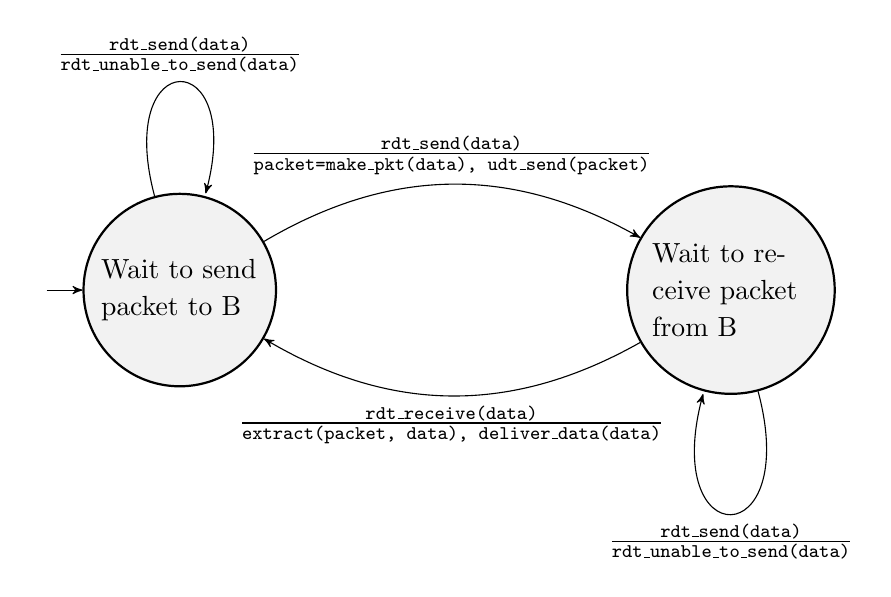
\begin{tikzpicture}[node distance=7cm]
    \node[state, initial, text width=2cm] (snd) {Wait to send packet to B};
    \node[state, right of=snd, text width=2cm] (rcv) {Wait to receive packet from B};

    \draw (snd) edge[loop above] node {$\frac{\texttt{rdt\_send(data)}}{\texttt{rdt\_unable\_to\_send(data)}}$} (snd);
    \draw (rcv) edge[loop below] node {$\frac{\texttt{rdt\_send(data)}}{\texttt{rdt\_unable\_to\_send(data)}}$} (rcv);
    \draw (snd) edge[bend left, above] node {$\frac{\texttt{rdt\_send(data)}}{\texttt{packet=make\_pkt(data), udt\_send(packet)}}$} (rcv);
    \draw (rcv) edge[bend left, below] node {$\frac{\texttt{rdt\_receive(data)}}{\texttt{extract(packet, data), deliver\_data(data)}}$} (snd);
\end{tikzpicture}    
\end{center}
FSM for B:
\begin{center}
\begin{tikzpicture}[node distance=1cm]
    \node[state, right of=rcv, text width=2cm] (snd) {Wait to send packet to B};
    \node[state, initial, text width=2cm] (rcv) {Wait to receive packet from B};

    \draw (snd) edge[loop above] node {$\frac{\texttt{rdt\_send(data)}}{\texttt{rdt\_unable\_to\_send(data)}}$} (snd);
    \draw (rcv) edge[loop below] node {$\frac{\texttt{rdt\_send(data)}}{\texttt{rdt\_unable\_to\_send(data)}}$} (rcv);
    \draw (snd) edge[bend left, above] node {$\frac{\texttt{rdt\_send(data)}}{\texttt{packet=make\_pkt(data), udt\_send(packet)}}$} (rcv);
    \draw (rcv) edge[bend left, below] node {$\frac{\texttt{rdt\_receive(data)}}{\texttt{extract(packet, data), deliver\_data(data)}}$} (snd);
\end{tikzpicture}    
\end{center}


\subsubsection{In the generic SR protocol that we studied in Section 3.4.4, the sender transmits a message as soon as it is available (if it is in the window) without waiting for an acknowledgment. Suppose now that we want an SR protocol that sends messages two at a time. That is, the sender will send a pair of messages and will send the next pair of messages only when it knows that both messages in the first pair have been received correctly. Suppose that the channel may lose messages but will not corrupt or reorder messages. Design an error-control protocol for the unidirectional reliable transfer of messages. Give an FSM description of the sender and receiver. Describe the format of the packets sent between sender and receiver, and vice versa. If you use any procedure calls other than those in Section 3.4  (for example, \texttt{udt\_send()}, \texttt{start\_timer()}, \texttt{rdt\_rcv()}, and so on), clearly state their actions. Give an example (a timeline trace of sender and receiver) showing how your protocol recovers from a lost packet. (P18)}

The sender waits until it receives an ACK for a pair of messages (seqnum and seqnum + 1) before moving on to the next pair. Data packets have a data field with a two-bit sequence number, so that we can express the sequence numbers 0, 1, 2 and 3. Four distinct sequence numbers are necessary to distinguish in which pair of messages that might have been lost. \\
\\
The sender state records whether:
\begin{itemize}
    \item No ACKs have been received for the current pair
    \item Only an ACK for seqnum and not seqnum + 1 has been received.
    \item Only an ACK for seqnum + 1 and not seqnum has been received.
\end{itemize}
It is assumed that seqnum is initially 0 and that the sender has sent the first two data messages. \\
\\
FSM for the sender: \\
\begin{center}
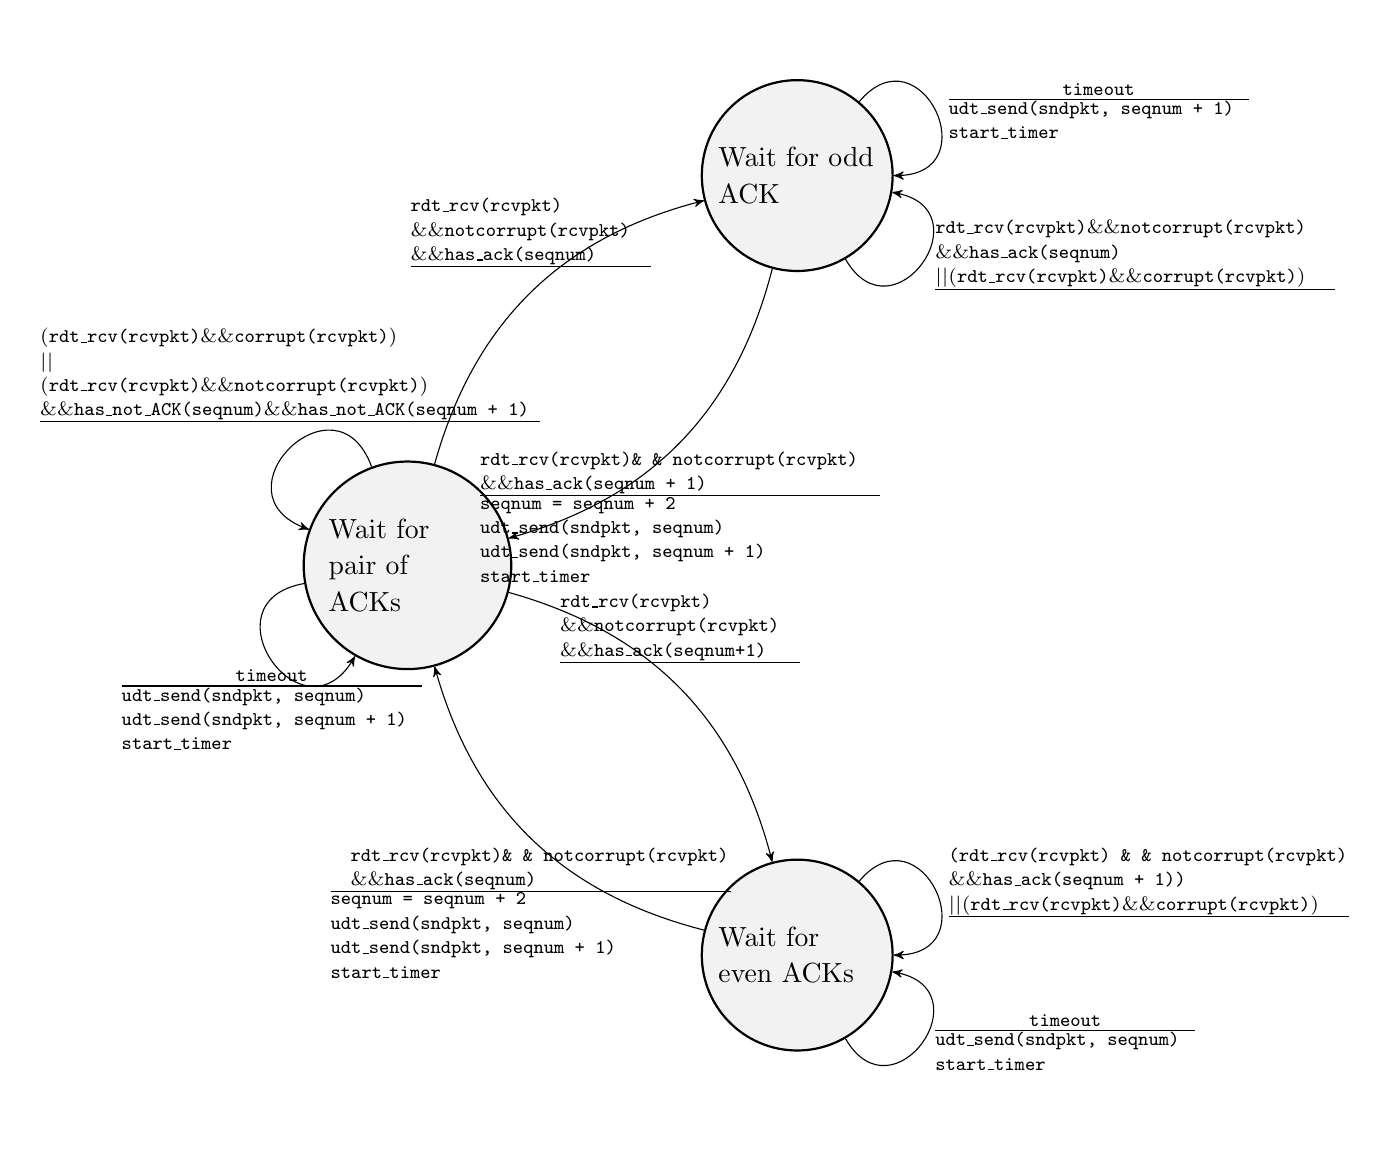
\begin{tikzpicture}[node distance=7cm]
    \node[state, text width=2cm] (pair) {Wait for pair of ACKs};
    \node[state, above right of=pair, text width=2cm] (odd) {Wait for odd ACK};
    \node[state, below right of=pair, text width=2cm] (even) {Wait for even ACKs};

    \draw (pair) edge[out=110, in=520, looseness=3] node[above] {$
        \frac{
            \parbox{2.5in \scriptsize}{($\texttt{rdt\_rcv(rcvpkt)} \&\& \texttt{corrupt(rcvpkt)})$ \\
            $||$ \\
            $\lr{ \texttt{rdt\_rcv(rcvpkt)} \&\& \texttt{notcorrupt(rcvpkt)}}$ \\
            $ \& \& \texttt{has\_not\_ACK(seqnum)} \& \& \texttt{has\_not\_ACK(seqnum + 1)}$
            }}{
        }
    $} (pair);
    \draw (pair) edge[out=550, in=600, looseness=3] node[below] {$
        \frac{
            \texttt{timeout}
            }{
                \parbox{1.5in \scriptsize}{$\texttt{udt\_send(sndpkt, seqnum)}$ \\
                $\texttt{udt\_send(sndpkt, seqnum + 1)}$ \\
                $\texttt{start\_timer}$
            }}$
    } (pair);

    \draw (odd) edge[out=50, in=0, looseness=3] node[right] {$
        \frac{
            \texttt{timeout}
        }{\parbox{1.5in \scriptsize}{
            $\texttt{udt\_send(sndpkt, seqnum + 1)}$ \\
            $\texttt{start\_timer}$
        }}$} (odd);
    \draw (odd) edge[out=-60, in=-10, looseness=3] node[right] {$
        \frac{\parbox{2in \scriptsize}{
            $\texttt{\texttt{rdt\_rcv(rcvpkt)}} \& \& \texttt{notcorrupt(rcvpkt)}$ \\
            $ \& \& \texttt{has\_ack(seqnum)}$ \\
            $|| (\texttt{rdt\_rcv(rcvpkt)} \& \& \texttt{corrupt(rcvpkt)})$
            }}{
            }$} (odd);

    \draw (even) edge[out=50, in=0, looseness=3] node[right] {$
        \frac{\parbox{2in \scriptsize}{
            $\texttt{(\texttt{rdt\_rcv(rcvpkt)} \& \& notcorrupt(rcvpkt)}$ \\
            $\& \& \texttt{has\_ack(seqnum + 1))}$ \\
            $|| (\texttt{rdt\_rcv(rcvpkt)} \& \& \texttt{corrupt(rcvpkt)})$
            }}{
        }$} (even);
    \draw (even) edge[out=-60, in=-10, looseness=3] node[right] {$
    \frac{
        \texttt{timeout}
    }{\parbox{1.3in \scriptsize}{
        $\texttt{udt\_send(sndpkt, seqnum)}$ \\
        $\texttt{start\_timer}$   
    }}$} (even);

    \draw (pair) edge[bend left, above] node[above] {$
    \frac{\parbox{1.2in \scriptsize}{
        $\texttt{rdt\_rcv(rcvpkt)}$ \\
        $\& \& \texttt{notcorrupt(rcvpkt)}$ \\
        $\& \& \texttt{has\_ack(seqnum)}$
    }}{
    }$} (odd);
    \draw (odd) edge[bend left, below] node[below] {$
    \frac{\parbox{2in \scriptsize}{
        $\texttt{rdt\_rcv(rcvpkt)$ \\ 
        $\& \& notcorrupt(rcvpkt)}$ \\
        $\& \& \texttt{has\_ack(seqnum + 1)}$
    }}{\parbox{2in \scriptsize}{
        $\texttt{seqnum = seqnum + 2}$ \\
        $\texttt{udt\_send(sndpkt, seqnum)}$ \\
        $\texttt{udt\_send(sndpkt, seqnum + 1)}$ \\
        $\texttt{start\_timer}$
    }}$} (pair);

    \draw (pair) edge[bend left, above] node[above] {$
    \frac{\parbox{1.2in \scriptsize}{
        $\texttt{rdt\_rcv(rcvpkt)}$ \\
        $\& \& \texttt{notcorrupt(rcvpkt)}$ \\
        $\& \& \texttt{has\_ack(seqnum+1)}$
    }}{
    }$} (even);
    \draw (even) edge[bend left, below] node[below] {$
    \frac{\parbox{1.8in \scriptsize}{
        $\texttt{rdt\_rcv(rcvpkt)$ \\
        $\& \& \texttt{notcorrupt(rcvpkt)}}$ \\
        $\& \& \texttt{has\_ack(seqnum)}$
    }}{\parbox{2in \scriptsize}{
        $\texttt{seqnum = seqnum + 2}$ \\
        $\texttt{udt\_send(sndpkt, seqnum)}$ \\   
        $\texttt{udt\_send(sndpkt, seqnum + 1)}$ \\
        $\texttt{start\_timer}$  
    }}$} (pair);
\end{tikzpicture}    
\end{center}
FSM for the receiver:
\begin{center}
    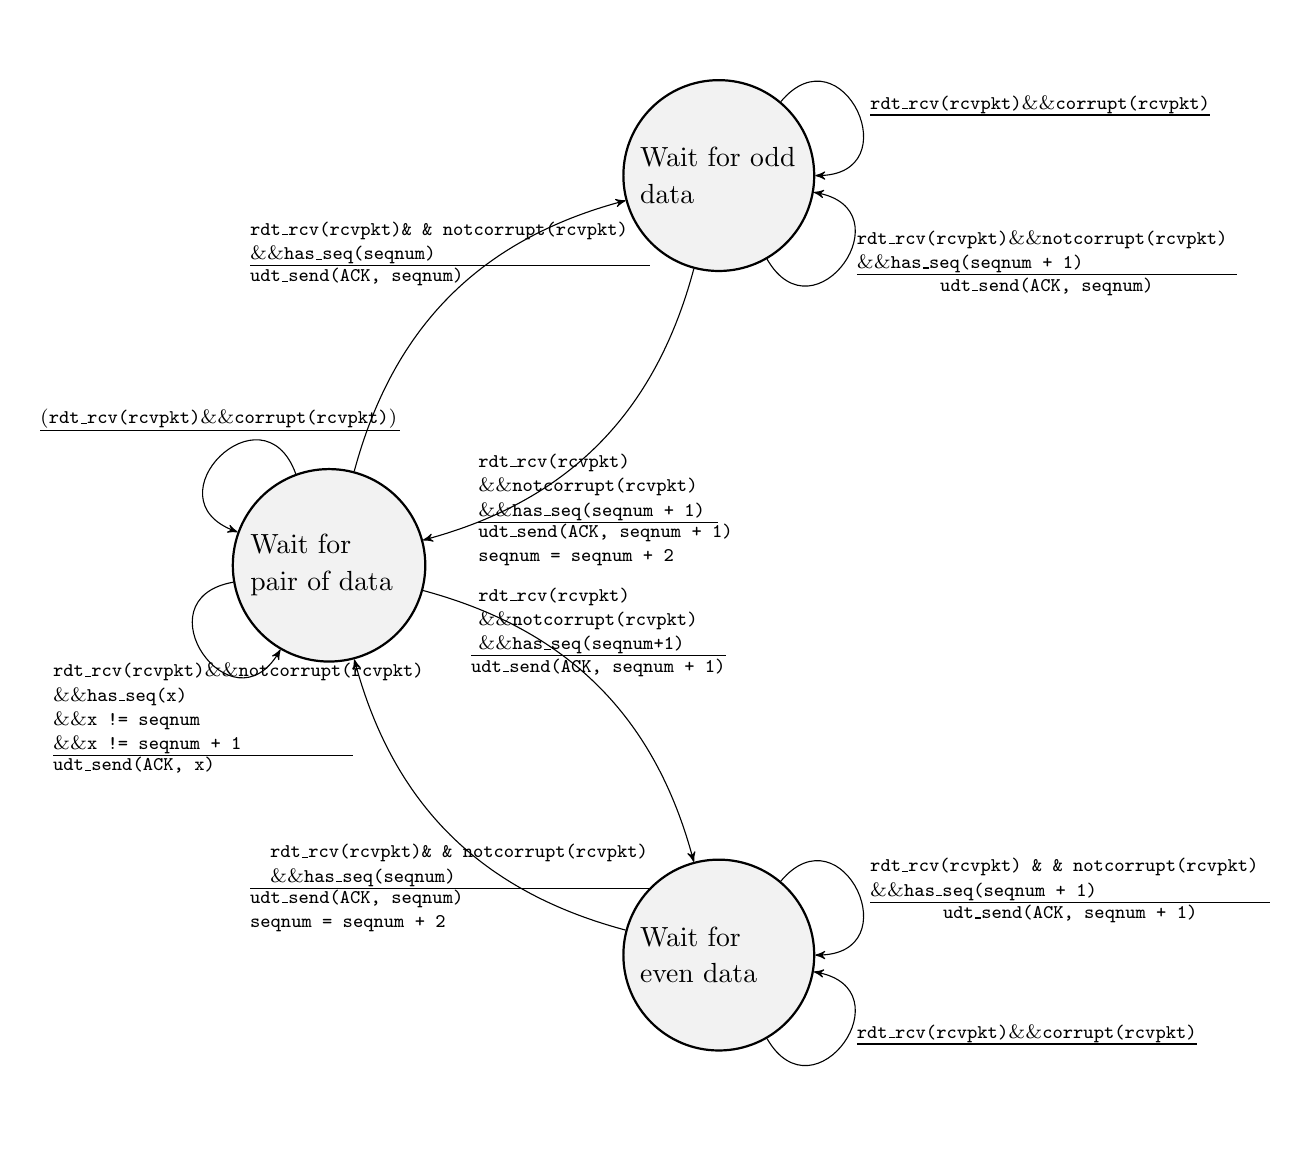
\begin{tikzpicture}[node distance=7cm]
        \node[state, text width=2cm] (pair) {Wait for pair of data};
        \node[state, above right of=pair, text width=2cm] (odd) {Wait for odd data};
        \node[state, below right of=pair, text width=2cm] (even) {Wait for even data};
    
        \draw (pair) edge[out=110, in=520, looseness=3] node[above] {$
            \frac{\parbox{1.8in \scriptsize}{
                ($\texttt{rdt\_rcv(rcvpkt)} \&\& \texttt{corrupt(rcvpkt)})$ 
                }}{
            }
        $} (pair);
        \draw (pair) edge[out=550, in=600, looseness=3] node[below] {$
            \frac{\parbox{1.5in \scriptsize}{
                $\texttt{rdt\_rcv(rcvpkt)} \& \& \texttt{notcorrupt(rcvpkt)}$ \\
                $\& \& \texttt{has\_seq(x)}$ \\
                $\& \& \texttt{x != seqnum}$ \\
                $\& \& \texttt{x != seqnum + 1}$
                }}{\parbox{1.5in \scriptsize}{
                    $\texttt{udt\_send(ACK, x)}$ \\
                }}$
        } (pair);
    
        \draw (odd) edge[out=50, in=0, looseness=3] node[right] {$
            \frac{
                \texttt{rdt\_rcv(rcvpkt)} \& \& \texttt{corrupt(rcvpkt)}
            }{\parbox{1.5in \scriptsize}{
            }}$} (odd);
        \draw (odd) edge[out=-60, in=-10, looseness=3] node[right] {$
            \frac{\parbox{1.9in \scriptsize}{
                $\texttt{\texttt{rdt\_rcv(rcvpkt)}} \& \& \texttt{notcorrupt(rcvpkt)}$ \\
                $ \& \& \texttt{has\_seq(seqnum + 1)}$ 
                }}{
                    \texttt{udt\_send(ACK, seqnum)}
                }$} (odd);
    
        \draw (even) edge[out=50, in=0, looseness=3] node[right] {$
            \frac{\parbox{2in \scriptsize}{
                $\texttt{\texttt{rdt\_rcv(rcvpkt)} \& \& notcorrupt(rcvpkt)}$ \\
                $\& \& \texttt{has\_seq(seqnum + 1)}$
                }}{
                    \texttt{udt\_send(ACK, seqnum + 1)}
            }$} (even);
        \draw (even) edge[out=-60, in=-10, looseness=3] node[right] {$
        \frac{
            \texttt{rdt\_rcv(rcvpkt)} \& \& \texttt{corrupt(rcvpkt)}
        }{
        }$} (even);
    
        \draw (pair) edge[bend left, above] node[above] {$
        \frac{\parbox{2in \scriptsize}{
            $\texttt{rdt\_rcv(rcvpkt)$ \\ 
            $\& \& notcorrupt(rcvpkt)}$ \\
            $\& \& \texttt{has\_seq(seqnum)}$
        }}{\parbox{2in \scriptsize}{
            $\texttt{udt\_send(ACK, seqnum)}$ 
        }}$} (odd);
        \draw (odd) edge[bend left, below] node[below] {$
        \frac{\parbox{1.2in \scriptsize}{
            $\texttt{rdt\_rcv(rcvpkt)}$ \\
            $\& \& \texttt{notcorrupt(rcvpkt)}$ \\
            $\& \& \texttt{has\_seq(seqnum + 1)}$
        }}{\parbox{1.2in \scriptsize}{
            $\texttt{udt\_send(ACK, seqnum + 1)}$ \\
            $\texttt{seqnum = seqnum + 2}$
        }}$} (pair);
    
        \draw (pair) edge[bend left, above] node[above] {$
        \frac{\parbox{1.2in \scriptsize}{
            $\texttt{rdt\_rcv(rcvpkt)}$ \\
            $\& \& \texttt{notcorrupt(rcvpkt)}$ \\
            $\& \& \texttt{has\_seq(seqnum+1)}$
        }}{
            \texttt{udt\_send(ACK, seqnum + 1)}
        }$} (even);
        \draw (even) edge[bend left, below] node[below] {$
        \frac{\parbox{1.8in \scriptsize}{
            $\texttt{rdt\_rcv(rcvpkt)$ \\
            $\& \& \texttt{notcorrupt(rcvpkt)}}$ \\
            $\& \& \texttt{has\_seq(seqnum)}$
        }}{\parbox{2in \scriptsize}{
            $\texttt{udt\_send(ACK, seqnum)}$ \\  
            $\texttt{seqnum = seqnum + 2}$ \\  
        }}$} (pair);
\end{tikzpicture}    
\end{center}
Timing diagram:

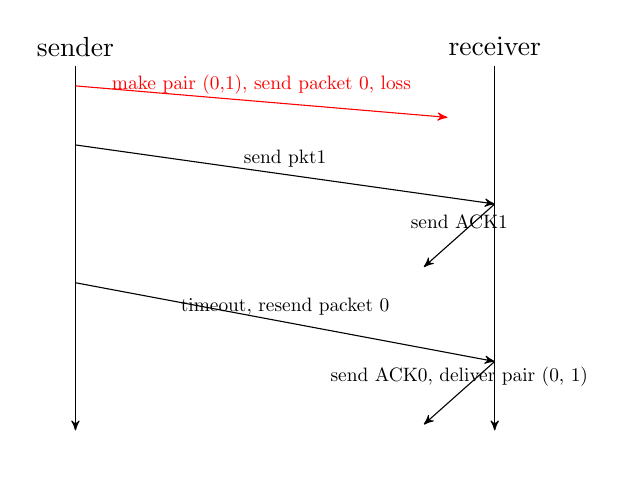
\begin{tikzpicture}[node distance=4cm,auto,>=stealth']
    \node[] (receiver) {receiver};
    \node[left = of receiver] (sender) {sender};
    \node[below of=receiver, node distance=5cm] (receiver_ground) {};
    \node[below of=sender, node distance=5cm] (sender_ground) {};
    %
    \draw (sender) -- (sender_ground);
    \draw (receiver) -- (receiver_ground);
    \draw[->, red] ($(sender)!0.1!(sender_ground)$) -- node[above,scale=0.7, midway]{make pair (0,1), send packet 0, loss} (-0.6, -0.9);
    \draw[->] ($(sender)!0.25!(sender_ground)$) -- node[above,scale=0.7, midway]{send pkt1} ($(receiver)!0.4!(receiver_ground)$);
    \draw[<-] (-0.9, -2.8) -- node[above,scale=0.7,midway]{send ACK1} ($(receiver)!0.4!(receiver_ground)$);
    \draw[->] ($(sender)!0.6!(sender_ground)$) -- node[above,scale=0.7, midway]{timeout, resend packet 0} ($(receiver)!0.8!(receiver_ground)$);
    \draw[<-] (-0.9, -4.8) -- node[above,scale=0.7,midway]{send ACK0, deliver pair (0, 1)} ($(receiver)!0.8!(receiver_ground)$);
\end{tikzpicture}



\subsubsection{Suppose Host A and Host B use a GBN protocol with window size $N = 3$ and a long-enough range of sequence numbers. Assume Host A sends six application messages to Host B and that all messages are correctly received, except for the first acknowledgment and the fifth data segment. Draw a timing diagram (similar to Figure 3.22), showing the data segments and the acknowledgments sent along with the corresponding sequence and acknowledge numbers, respectively. (P19)}

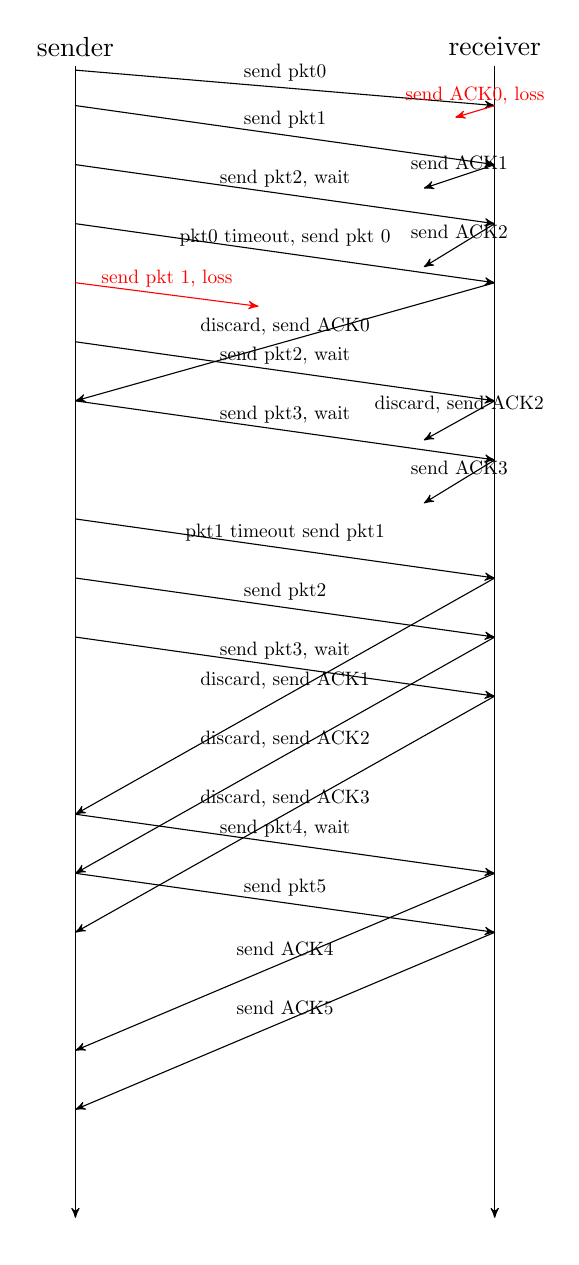
\begin{tikzpicture}[node distance=4cm,auto,>=stealth']
    \node[] (receiver) {receiver};
    \node[left = of receiver] (sender) {sender};
    \node[below of=receiver, node distance=15cm] (receiver_ground) {};
    \node[below of=sender, node distance=15cm] (sender_ground) {};
    %
    \draw (sender) -- (sender_ground);
    \draw (receiver) -- (receiver_ground);
    \draw[->] ($(sender)!0.02!(sender_ground)$) -- node[above,scale=0.7, midway]{send pkt0} ($(receiver)!0.05!(receiver_ground)$);
    \draw[<-, red] (-0.5, -0.9) -- node[above,scale=0.7,midway]{send ACK0, loss} ($(receiver)!0.05!(receiver_ground)$);
    \draw[->] ($(sender)!0.05!(sender_ground)$) -- node[above,scale=0.7, midway]{send pkt1} ($(receiver)!0.1!(receiver_ground)$);
    \draw[<-] (-0.9, -1.8) -- node[above,scale=0.7,midway]{send ACK1} ($(receiver)!0.1!(receiver_ground)$);
    \draw[->] ($(sender)!0.1!(sender_ground)$) -- node[above,scale=0.7, midway]{send pkt2, wait} ($(receiver)!0.15!(receiver_ground)$);
    \draw[<-] (-0.9, -2.8) -- node[above,scale=0.7,midway]{send ACK2} ($(receiver)!0.15!(receiver_ground)$);
    \draw[->] ($(sender)!0.15!(sender_ground)$) -- node[above,scale=0.7, midway]{pkt0 timeout, send pkt 0} ($(receiver)!0.2!(receiver_ground)$);
    \draw[<-] ($(sender)!0.3!(sender_ground)$) -- node[above,scale=0.7,midway]{discard, send ACK0} ($(receiver)!0.2!(receiver_ground)$);
    \draw[->, red] ($(sender)!0.2!(sender_ground)$) -- node[above,scale=0.7, midway]{send pkt 1, loss} (-3, -3.3);
    \draw[->] ($(sender)!0.25!(sender_ground)$) -- node[above,scale=0.7, midway]{send pkt2, wait} ($(receiver)!0.3!(receiver_ground)$);
    \draw[<-] (-0.9, -5.0) -- node[above,scale=0.7,midway]{discard, send ACK2} ($(receiver)!0.3!(receiver_ground)$);
    \draw[->] ($(sender)!0.3!(sender_ground)$) -- node[above,scale=0.7, midway]{send pkt3, wait} ($(receiver)!0.35!(receiver_ground)$);
    \draw[<-] (-0.9, -5.8) -- node[above,scale=0.7,midway]{send ACK3} ($(receiver)!0.35!(receiver_ground)$);
    \draw[->] ($(sender)!0.4!(sender_ground)$) -- node[above,scale=0.7, midway]{pkt1 timeout send pkt1} ($(receiver)!0.45!(receiver_ground)$);
    \draw[<-] ($(sender)!0.65!(sender_ground)$) -- node[above,scale=0.7,midway]{discard, send ACK1} ($(receiver)!0.45!(receiver_ground)$);
    \draw[->] ($(sender)!0.45!(sender_ground)$) -- node[above,scale=0.7, midway]{send pkt2} ($(receiver)!0.50!(receiver_ground)$);
    \draw[<-] ($(sender)!0.70!(sender_ground)$) -- node[above,scale=0.7,midway]{discard, send ACK2} ($(receiver)!0.50!(receiver_ground)$);
    \draw[->] ($(sender)!0.50!(sender_ground)$) -- node[above,scale=0.7, midway]{send pkt3, wait} ($(receiver)!0.55!(receiver_ground)$);
    \draw[<-] ($(sender)!0.75!(sender_ground)$) -- node[above,scale=0.7,midway]{discard, send ACK3} ($(receiver)!0.55!(receiver_ground)$);
    \draw[->] ($(sender)!0.65!(sender_ground)$) -- node[above,scale=0.7, midway]{send pkt4, wait} ($(receiver)!0.70!(receiver_ground)$);
    \draw[<-] ($(sender)!0.85!(sender_ground)$) -- node[above,scale=0.7,midway]{send ACK4} ($(receiver)!0.70!(receiver_ground)$);
    \draw[->] ($(sender)!0.70!(sender_ground)$) -- node[above,scale=0.7, midway]{send pkt5} ($(receiver)!0.75!(receiver_ground)$);
    \draw[<-] ($(sender)!0.90!(sender_ground)$) -- node[above,scale=0.7,midway]{send ACK5} ($(receiver)!0.75!(receiver_ground)$);
\end{tikzpicture}



\subsubsection{Consider a scenario in which Host A and Host B want to send messages to Host C. Hosts A and C are connected by a channel that can lose and corrupt (but not reorder) messages. Hosts B and C are connected by another channel (independent of the channel connecting A and C) with the same properties. The transport layer at Host C should alternate in delivering messages from  A and B to the layer above (that is, it should first deliver the data from a packet from A, then the data from a packet from B, and so on). Design a stop-and-wait-like error-control protocol for reliably transferring packets from A and B to C, with alternating delivery at C as described above. Give FSM descriptions of A and C. (Hint: The FSM for B should be essentially the same as  for A.) Also, give a description of the packet format(s) used. (P20)}

\begin{center}
    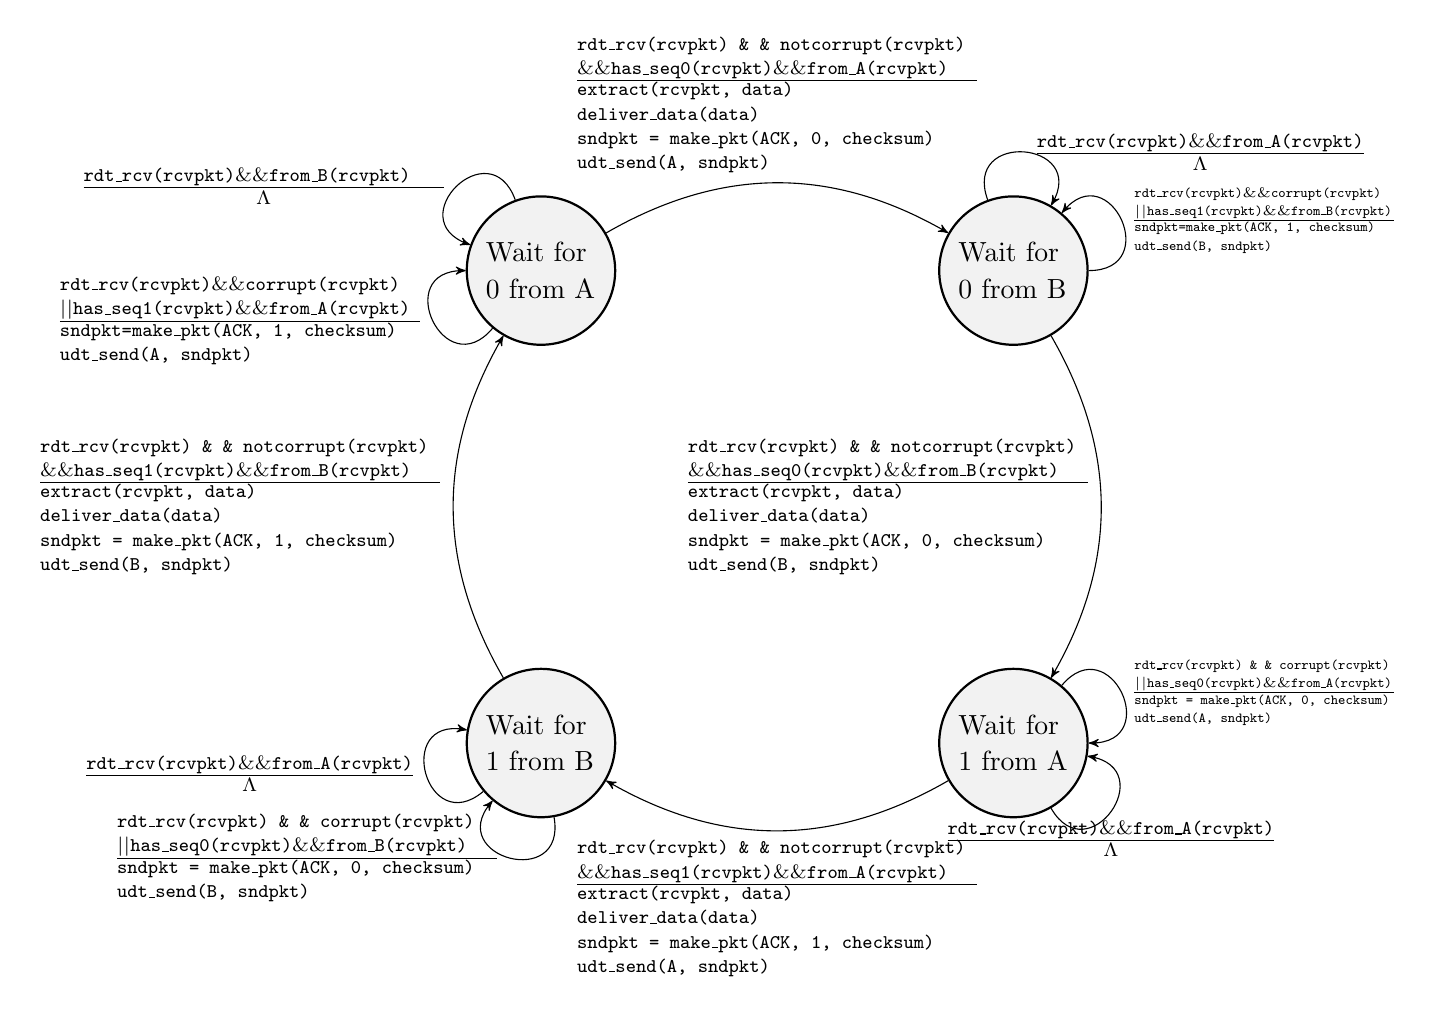
\begin{tikzpicture}[node distance=6cm]
        \node[state, text width=1.4cm] (0A) {Wait for 0 from A};
        \node[state, right of=0A, text width=1.4cm] (0B) {Wait for 0 from B};
        \node[state, below of=0A, text width=1.4cm] (1B) {Wait for 1 from B};
        \node[state, right of=1B, text width=1.4cm] (1A) {Wait for 1 from A};
    
        \draw (0A) edge[out=110, in=520, looseness=3] node[left] {$
            \frac{\parbox{1.8in \scriptsize}{
                $\texttt{rdt\_rcv(rcvpkt)} \&\& \texttt{from\_B(rcvpkt)}$ 
                }}{
                    \Lambda
            }
        $} (0A);
        \draw (0A) edge[out=590, in=540, looseness=3] node[left] {$
            \frac{\parbox{1.8in \scriptsize}{
                $\texttt{rdt\_rcv(rcvpkt)} \& \& \texttt{corrupt(rcvpkt)}$ \\
                $|| \texttt{has\_seq1(rcvpkt)} \& \& \texttt{from\_A(rcvpkt)}$
                }}{\parbox{1.8in \scriptsize}{
                    $\texttt{sndpkt=make\_pkt(ACK, 1, checksum)}$ \\
                    $\texttt{udt\_send(A, sndpkt)}$
                }}$
        } (0A);
    
        \draw (0B) edge[out=110, in=60, looseness=3] node[right] {$
            \frac{
                \texttt{rdt\_rcv(rcvpkt)} \& \& \texttt{from\_A(rcvpkt)}
            }{
                \Lambda
            }$} (0B);
        \draw (0B) edge[out=0, in=50, looseness=3] node[right] {$
            \frac{\parbox{1.3in \tiny}{
                $\texttt{\texttt{rdt\_rcv(rcvpkt)}} \& \& \texttt{corrupt(rcvpkt)}$ \\
                $ || \texttt{has\_seq1(rcvpkt)} \& \& \texttt{from\_B(rcvpkt)}$ 
                }}{\parbox{1.3in \tiny}{
                    $\texttt{sndpkt=make\_pkt(ACK, 1, checksum)}$ \\
                    $\texttt{udt\_send(B, sndpkt)}$
                }}$} (0B);
    
        \draw (1A) edge[out=50, in=0, looseness=3] node[right] {$
            \frac{\parbox{1.3in \tiny}{
                $\texttt{\texttt{rdt\_rcv(rcvpkt)} \& \& corrupt(rcvpkt)}$ \\
                $|| \texttt{has\_seq0(rcvpkt)} \& \& \texttt{from\_A(rcvpkt)}$
                }}{\parbox{1.3in \tiny}{
                    $\texttt{sndpkt = make\_pkt(ACK, 0, checksum)}$ \\
                    $\texttt{udt\_send(A, sndpkt)}$
                }}$} (1A);
        \draw (1A) edge[out=-60, in=-10, looseness=3] node[below] {$
        \frac{
            \texttt{rdt\_rcv(rcvpkt)} \& \& \texttt{from\_A(rcvpkt)}
        }{
            \Lambda
        }$} (1A);

        \draw (1B) edge[out=-80, in=-130, looseness=3] node[left] {$
            \frac{\parbox{1.9in \scriptsize}{
                $\texttt{\texttt{rdt\_rcv(rcvpkt)} \& \& corrupt(rcvpkt)}$ \\
                $|| \texttt{has\_seq0(rcvpkt)} \& \& \texttt{from\_B(rcvpkt)}$
                }}{\parbox{1.9in \scriptsize}{
                    $\texttt{sndpkt = make\_pkt(ACK, 0, checksum)}$ \\
                    $\texttt{udt\_send(B, sndpkt)}$
                }}$} (1B);
        \draw (1B) edge[out=-140, in=-190, looseness=3] node[left] {$
        \frac{
            \texttt{rdt\_rcv(rcvpkt)} \& \& \texttt{from\_A(rcvpkt)}
        }{
            \Lambda
        }$} (1B);
    
        \draw (0A) edge[bend left, above] node[above] {$
        \frac{\parbox{2in \scriptsize}{
            $\texttt{rdt\_rcv(rcvpkt) \& \& notcorrupt(rcvpkt)}$ \\
            $\& \& \texttt{has\_seq0(rcvpkt)} \& \& \texttt{from\_A(rcvpkt)}$
        }}{\parbox{2in \scriptsize}{
            $\texttt{extract(rcvpkt, data)}$ \\
            $\texttt{deliver\_data(data)}$ \\
            $\texttt{sndpkt = make\_pkt(ACK, 0, checksum)}$ \\
            $\texttt{udt\_send(A, sndpkt)}$
        }}$} (0B);
        
        \draw (0B) edge[bend left, above] node[left] {$
        \frac{\parbox{2in \scriptsize}{
            $\texttt{rdt\_rcv(rcvpkt) \& \& notcorrupt(rcvpkt)}$ \\
            $\& \& \texttt{has\_seq0(rcvpkt)} \& \& \texttt{from\_B(rcvpkt)}$
        }}{\parbox{2in \scriptsize}{
            $\texttt{extract(rcvpkt, data)}$ \\
            $\texttt{deliver\_data(data)}$ \\
            $\texttt{sndpkt = make\_pkt(ACK, 0, checksum)}$ \\
            $\texttt{udt\_send(B, sndpkt)}$
        }}$} (1A);

        \draw (1A) edge[bend left, above] node[below] {$
        \frac{\parbox{2in \scriptsize}{
            $\texttt{rdt\_rcv(rcvpkt) \& \& notcorrupt(rcvpkt)}$ \\
            $\& \& \texttt{has\_seq1(rcvpkt)} \& \& \texttt{from\_A(rcvpkt)}$
        }}{\parbox{2in \scriptsize}{
            $\texttt{extract(rcvpkt, data)}$ \\
            $\texttt{deliver\_data(data)}$ \\
            $\texttt{sndpkt = make\_pkt(ACK, 1, checksum)}$ \\
            $\texttt{udt\_send(A, sndpkt)}$
        }}$} (1B);

        \draw (1B) edge[bend left, above] node[left] {$
        \frac{\parbox{2in \scriptsize}{
            $\texttt{rdt\_rcv(rcvpkt) \& \& notcorrupt(rcvpkt)}$ \\
            $\& \& \texttt{has\_seq1(rcvpkt)} \& \& \texttt{from\_B(rcvpkt)}$
        }}{\parbox{2in \scriptsize}{
            $\texttt{extract(rcvpkt, data)}$ \\
            $\texttt{deliver\_data(data)}$ \\
            $\texttt{sndpkt = make\_pkt(ACK, 1, checksum)}$ \\
            $\texttt{udt\_send(B, sndpkt)}$
        }}$} (0A);
\end{tikzpicture}    
\end{center}




\subsubsection{Suppose we have two network entities, A and B. B has a supply of data messages that will be sent to A according to the following conventions. When A gets a request from the layer above to get the next data (D) message from B, A must send a request (R) message to B on the A-to-B channel. Only when B receives an R message can it send a data (D) message back to A on the B-to-A channel. A should deliver exactly one copy of each D message to the layer above. R messages can be lost (but not corrupted) in the A-to-B channel; D messages, once sent, are always delivered correctly. The delay along both channels is unknown and variable. Design (give an FSM description of) a protocol that incorporates the appropriate mechanisms to compensate for the loss-prone A-to-B channel and implements message passing to the layer above at entity A, as discussed above. Use only those mechanisms that are absolutely necessary. (21)}

Due to potential message loss in the A-to-B channel, A may need to retransmit its requests and could inadvertently send duplicate requests due to variable and unknown channel delays. To detect duplicates, the protocol employs sequence numbers, where a 1-bit sequence number suffices for a stop-and-wait type of protocol. \\
\\
A (the requestor) operates in four states:
\begin{enumerate}
    \item \textbf{"Wait for Request 0 from above"}: A waits for a request from above to send a data unit. Upon receiving the request, it sends a request message (R0) to B, starts a timer, and transitions to the "Wait for D0" state. It disregards anything received from B in this state.
    \item \textbf{"Wait for D0"}: A waits for a D0 data message from B, with a running timer. If the timer expires, A resends an R0 message, restarts the timer, and stays in this state. Upon receiving a D0 message, A stops the timer and transitions to "Wait for Request 1 from above". D1 messages received in this state are ignored.
    \item \textbf{"Wait for Request 1 from above"}: A waits for another request from above. Upon receiving it, it sends a request message (R1) to B, starts a timer, and transitions to "Wait for D1". It ignores messages from B in this state.
    \item \textbf{"Wait for D1"}: A waits for a D1 data message from B, with a running timer. If the timer expires, A resends an R1 message, restarts the timer, and stays in this state. Upon receiving a D1 message, A stops the timer and transitions to "Wait for Request 0 from above". D0 messages received in this state are ignored.
\end{enumerate}

The data supplier (B) operates in two states:
\begin{enumerate}
    \item \textbf{"Send D0"}: B responds to R0 messages by sending D0 and remains in this state. Upon receiving an R1 message, it discards the D0 data (since it's already been received) and transitions to "Send D1" to send the next requested data piece.
    \item \textbf{"Send D1"}: B responds to R1 messages by sending D1 and remains in this state. Upon receiving another R1 message, it transitions back to "Send D1".
\end{enumerate}



\subsubsection{Consider the GBN protocol with a sender window size of 4 and a sequence number range of 1,024. Suppose that at time $t$, the next in-order packet that the receiver is expecting has a sequence number of $k$. Assume that the medium does not reorder messages. Answer the following questions: (P22)}

\textbf{a. What are the possible sets of sequence numbers inside the sender's window at time $t$? Justify your answer.} \\
If the receiver have received and ACKed the preceding $k-1$ packets and these ACKs have been received by the sender, then the sender's window is $[k, k - 1 + N]$, where $N$ is the window size. Since $N = 4$ we have $[k, k + 3]$. \\
\\
If no ACKs from preceding $k - 1$ packets have been received by the sender, then the sender's window is $[k - N, k - 1]$ in the general case and in our case $[k - 4, k - 1]$.
\\
Since these are the two extremes of the sets of sequence numbers we can combine the end points for these intervals and the possible sets of sequence numbers in the sender's window will be $[k - N, k - 1 + N]$. \\
\\
\textbf{b. What are all possible values of the ACK field in all possible messages currently propagating back to the sender at time $t$? Justify your answer.} \\
If the receiver have received and ACKed the preceding $k - 1$ packets then the earliest ACK will be $k - 1 - N$, since this is what is limited by a window size of $N$, and the latest ACK will be $k - 1$. So the propagating ACKs will have values in the range $[k - 1 - N, k - 1]$ which in our case with $N = 4$ is $[k - 5, k - 1]$.



\subsubsection{Give one example where buffering out-of-order segments would significantly improve the throughput of a GBN protocol. (P23)}

If a segment is delivered to the receiver but the corresponding ACK is lost. Then the proceeding segments that are send and ACKed are not buffered at thus decreases throughput significantly especially if the timeout is long and the window large.



\subsubsection{Consider a scenario where the three hosts A, B, and C are connected as a ring: A to B, B to C, and C to A. Assume that A and C run protocol \texttt{rdt3.0}, whereas B simply relays all messages received from A to C. (P24)}

\textbf{a. Does this arrangement enable reliable delivery of messages from A to C?} \\
When A transmits through B to C every mechanism (timeout and ACKs) that enable reliable data delivery are retransmitted by B, as they would be any node in the network, and therefore still works as intended, however timeout must account for the extra RTT that B introduces. \\
\\
Since C sends directly to A we have the case of 2 hosts that sends using \texttt{rdt3.0} which has reliable data transfer. Since B does not transmit data but simply relays it, we have no other cases to consider. Therefore we have that this arrangement enables reliable data transfer. \\
\\
\textbf{b. Can B tell if a certain message has been correctly received by A?} \\
\\
If A has received a message from C then it has been sent directly whereafter the ACK will be sent through B to C. Therefor B will know by receiving the ACK whether A has correctly received a message.



\subsubsection{We have said that an application may choose UDP for a transport protocol because UDP offers finer application control (than TCP) of what data is sent in a segment and when. (P25)}

\textbf{Why does an application have more control of what data is sent in a segment?} \\
In UDP the application have more control of the data sent in the segment, since a segment in UDP mostly contains the application data and not all the extra data that TCP adds for reliable data transfer and congestion control.\\
\\
\textbf{Why does an application have more control on when the segment is sent?} \\
Because UDP sends segments as soon as the application layer has handed its package to UDP. TCP on the other hand needs handshaking before sending and holds segments in a buffer before sending to implement reliable data transfer and congestion control.\\


\subsubsection{Consider transferring an enormous file of $L$ bytes from Host A to Host B. Assume an MSS of 536 bytes. (P26)}

\textbf{a. What is the maximum value of $L$ such that TCP sequence numbers are not exhausted? Recall that the TCP sequence number field has 4 bytes.} \\
Since TCP sequence number field has 4 bytes it can express $2^{4 \cdot 8} = 2^{32} = 4 \, 294 \, 967 \, 296$ numbers. Since the sequence numbers are incremented by the bytes of data sent the MSS is irrelevant, and $L$ is only limited by having fewer than $2^{32}$ bytes. \\
\\
\textbf{b. For the $L$ you obtain in (a), find how long it takes to transmit the file. Assume that a total of 66 bytes of transport, network, and data-link header are added to each segment before the resulting packet is sent out over a 155 Mbps link. Ignore flow control and congestion control so A can pump out the segments back to back and continuously.} 
\\
Since MSS is strictly the payload, we have that each segment is $536 + 66 = 602$ bytes. Since $L$ can max be $2^{32}$ we have that we must send $\ceil{\frac{2^{32}}{536}} = 8 \, 012 \,999$ segments for the total file to be transferred. Each of these segments are transferred over the 155 Mbps link in $\frac{602 \cdot 8 \, \text{bits}}{155 \cdot 10^6 \, \text{bits/s}} = 3.1 \cdot 10^{-5}$ seconds. This means that the whole file will be transferred in $8 \, 012 \, 999 \cdot 3.1 \cdot 10^{-5} = 248$ seconds.


\subsubsection{Host A and B are communicating over a TCP connection following RFC 5681. Host B has already received from A all bytes up through byte 96. Suppose Host A then sends two segments to Host B back-to-back. The first and the second segments contain 40 and 80 bytes of data, respectively. In the first segment, the sequence number is 97, the source port number is 302, and the destination port number is 80. Host B sends an acknowledgment whenever it receives a segment from Host A. (P27)}

\textbf{a. In the second segment sent from Host A to B, what are the sequence number, source port number, and destination port number?} \\
Since the first segment has sequence number 97 and contains 40 bytes of data then the receiver must afterwards have received bytes up through byte $96 + 40 = 136$. Therefore the first byte in the second segment will be byte 137 of the byte stream and therefore the sequence number for the second segment must be 137. \\
\\
The port numbers are identical to the ones for the first segment so the source port number is 302 and the destination port number is 80.
\\
\textbf{b. If the first segment arrives before the second segment, in the acknowledgment of the first arriving segment, what is the acknowledgment number, the source port number, and the destination port number?} \\
Acknowledgment numbers indicate the expected sequence number of the next package. Therefore the acknowledgment number for the first segment will be the sequence number for the second package which is 137.\\
\\
Since acknowledgments come from the receiver the port numbers have changed roles and therefore the source port number is 80 and the destination port number is 302. \\
\\
\textbf{c. If the second segment arrives before the first segment, in the acknowledgment of the first arriving segment, what is the acknowledgment number?} \\
If the second segment arrives before the first segment, then the sequence number of the first segment is what the receiver is waiting for. It will therefore retransfer an acknowledgment number equal to the sequence number of the first segment, which is 97, indicating that it is still waiting for that segment. \\
\\
\textbf{d. Suppose the two segments sent by A arrive in order at B. The first acknowledgment arrives after the first timeout interval. What is the sequence number of the next segment that A will transmit?} \\
Since the acknowledgment for the first segment arrives after a timeout, A will by the timeout have expected that the segment was lost and retransmitted it. The next segment A sends after the two segments is therefore a retransmit of the first segment, which has the same sequence of 97 as when it was initially transmitted.



\subsubsection{Host A and B are directly connected with a 10 Gbps link. There is one TCP connection between the two hosts, and Host A is sending to Host B an enormous file over this connection. Host A can send its application data into its TCP socket at a rate as high as 1 Gbps, but Host B can read out of its TCP receive buffer at a maximum rate of 600 Mbps. Describe the effect of TCP flow control. (P28)}

The implementation of buffers by TCP flow control reduce throughput in several ways. A can send files to its buffer slower than it can retransmit directly on the link. And even more restricting is the fact that B can read much slower from its buffer than A can transmit, which mean that B must repeatedly set the window size to 0 so that it can empty its buffer. The whole transmission is restricted by the reading speed of B and will long term on average be 600 Mbps. Without flow control A and B could communicate faster directly through the link at 10 Gbps.



\subsubsection{SYN cookies were discussed in Section 3.5.6. (P29)}

\textbf{a. Why is it necessary for the server to use a special initial sequence number in the SYNACK?} \\
The special initial sequence number is a hash of source and destination IPs and ports and is used to defend against SYN FLOOD attacks. \\
\\
\textbf{b. Suppose an attacker knows that a target host uses SYN cookies. Can the attacker create half-open or fully open connections by simply sending an ACK packet to the target? Why or why not?} \\
No. The attacker cannot open half-open connections since a server using SYN cookies does not maintain connection variables or buffers before a full connection is established. The attacker cannot establish a full connection either as this requires knowing the special initial sequence number.
\\
\textbf{c. Suppose an attacker collects a large amount of initial sequence numbers sent by the server. Can the attacker cause the server to create many fully open connections by sending ACKs with those initial sequence numbers? Why?} \\
Not if the server adds a time stamp when computing the initial sequence numbers and choosing an expiration time for these numbers. It can then discard the expired initial sequence numbers if the attacker replays them.



\subsubsection{Consider the network shown in Scenario 2 in Section 3.6.1. Suppose both sending hosts A and B have some fixed timeout values. (P30)}

\textbf{a. Argue that increasing the size of the finite buffer of the router might possibly decrease the throughput $(\lambda_{\text{out}})$.} \\
When buffers become too large packets can be held in the buffer for longer periods of time. When timeout is fixed it is possible that many more packets are retransmitted only because they have been kept in the buffer for too long and not because they have been lost. This increases congestion and number of duplicate packets on the links which increase queuing delay and eventually packet loss which overall lead to a decrease in throughput. Thus buffers might be increased to prevent congestion, but can with fixed timeout paradoxically lead to increased congestion instead. \\ 
\\
\textbf{b. Now suppose both hosts dynamically adjust their timeout values (like what TCP does) based on the buffering delay at the router. Would increasing the buffer size help to increase the throughput? Why?} \\
Yes, now timeout can be increased when segments remain longer in the buffer, so that these segments are not retransmitted because of buffering delay. The increase in buffer can now decrease packet loss and allow hosts to maintain high transmission rates during periods of congestion.

\subsubsection{Suppose that the five measured \texttt{SampleRTT} values (see Section 3.5.3) are 112 ms, 140 ms, 110 ms, 90 ms, and 90 ms. Compute the \texttt{EstimatedRTT} after each of these \texttt{SampleRTT} values is obtained, using a value of  $\alpha = 0.125$ and assuming that the value of \texttt{EstimatedRTT} was 120 ms just before the first of these five samples were obtained. Compute also the \texttt{DevRTT} after each sample is obtained, assuming a value of $\beta = 0.25$ and assuming the value of \texttt{DevRTT} was 6 ms just before the first of these five samples was obtained. Finally, compute the TCP \texttt{TimeoutInterval} after each of these samples is obtained. (P31)}

We denote the time at the first sample RTT of 112 ms at time $t$. \\
\\
First we calculate the \texttt{SampleRTT}s in ms by 
\begin{equation*}
\begin{split}
    E_t[RTT_{t+1}] &= (1 - \alpha) E_{t-1}[RTT_t] + \alpha RTT_t \\
    &= (1 - 0.125) \cdot 120 + 0.125 \cdot 112 \\
    &= 119
\end{split}
\end{equation*}

\begin{equation*}
\begin{split}
    E_{t+1}[RTT_{t+2}] &= (1 - \alpha) E_t[RTT_{t+1}] + \alpha RTT_{t+1} \\
    &= (1 - 0.125) \cdot 119 + 0.125 \cdot 140 \\
    &= 121.625
\end{split}
\end{equation*}

\begin{equation*}
    \begin{split}
        E_{t+2}[RTT_{t+3}] &= (1 - \alpha) E_{t+1}[RTT_{t+2}] + \alpha RTT_{t+2} \\
        &= (1 - 0.125) \cdot 121.625 + 0.125 \cdot 110 \\
        &= 120.172
\end{split}
\end{equation*}

\begin{equation*}
    \begin{split}
        E_{t+3}[RTT_{t+4}] &= (1 - \alpha) E_{t+2}[RTT_{t+3}] + \alpha RTT_{t+3} \\
        &= (1 - 0.125) \cdot 120.172 + 0.125 \cdot 90 \\
        &= 116.401
\end{split}
\end{equation*}

\begin{equation*}
    \begin{split}
        E_{t+4}[RTT_{t+5}] &= (1 - \alpha) E_{t+3}[RTT_{t+4}] + \alpha RTT_{t+4} \\
        &= (1 - 0.125) \cdot 116.401 + 0.125 \cdot 90 \\
        &= 113.101
\end{split}
\end{equation*}
\\
Then we calculate the \texttt{DevRTT} in ms by
\begin{equation*}
    \begin{split}
        \text{dev}_t(RTT_t) &= (1 - \beta) \text{dev}_{t-1}(RTT_{t-1}) \cdot \lra{RTT_t - E_{t-1}[RTT_t]} \\
        &=  (1 - 0.25) \cdot 6 + 0.25 \cdot \lra{112 - 120} \\
        &= 6.5
\end{split}
\end{equation*}

\begin{equation*}
    \begin{split}
        \text{dev}_{t+1}(RTT_{t+1}) &= (1 - \beta) \text{dev}_{t}(RTT_{t}) \cdot \lra{RTT_{t+1} - E_{t}[RTT_{t+1}]} \\
        &=  (1 - 0.25) \cdot 6.5 + 0.25 \cdot \lra{140 - 119} \\
        &= 10.125
\end{split}
\end{equation*}

\begin{equation*}
    \begin{split}
        \text{dev}_{t+2}(RTT_{t+2}) &= (1 - \beta) \text{dev}_{t+1}(RTT_{t+1}) \cdot \lra{RTT_{t+2} - E_{t+1}[RTT_{t+2}]} \\
        &=  (1 - 0.25) \cdot 10.125 + 0.25 \cdot \lra{110 - 121.625} \\
        &= 10.5
\end{split}
\end{equation*}

\begin{equation*}
    \begin{split}
        \text{dev}_{t+3}(RTT_{t+3}) &= (1 - \beta) \text{dev}_{t+2}(RTT_{t+2}) \cdot \lra{RTT_{t+3} - E_{t+2}[RTT_{t+3}]} \\
        &=  (1 - 0.25) \cdot 10.5 + 0.25 \cdot \lra{90 - 120.172} \\
        &= 15.418
\end{split}
\end{equation*}

\begin{equation*}
    \begin{split}
        \text{dev}_{t+4}(RTT_{t+4}) &= (1 - \beta) \text{dev}_{t+3}(RTT_{t+3}) \cdot \lra{RTT_{t+4} - E_{t+3}[RTT_{t+4}]} \\
        &=  (1 - 0.25) \cdot 15.418 + 0.25 \cdot \lra{90 - 116.401} \\
        &= 18.164
\end{split}
\end{equation*}
We can now calculate the \texttt{TimeoutInterval}s by 
\begin{equation*}
\begin{split}
    \texttt{TimeoutInterval}_t &= E_t[RTT_{t+1}] + 4 \cdot \text{dev}_t(\text{RTT}_t) \\
    &= 119 + 4 \cdot 6.5 \\
    &= 145
\end{split}
\end{equation*}

\begin{equation*}
    \begin{split}
        \texttt{TimeoutInterval}_{t+1} &= E_{t+1}[RTT_{t+2}] + 4 \cdot \text{dev}_{t+1}(\text{RTT}_{t+1}) \\
        &= 121.625 + 4 \cdot 10.125 \\
        &= 162.125
\end{split}
\end{equation*}

\begin{equation*}
    \begin{split}
        \texttt{TimeoutInterval}_{t+2} &= E_{t+2}[RTT_{t+3}] + 4 \cdot \text{dev}_{t+2}(\text{RTT}_{t+2}) \\
        &= 120.172 + 4 \cdot 10.5 \\
        &= 162.172
\end{split}
\end{equation*}

\begin{equation*}
    \begin{split}
        \texttt{TimeoutInterval}_{t+3} &= E_{t+3}[RTT_{t+4}] + 4 \cdot \text{dev}_{t+3}(\text{RTT}_{t+3}) \\
        &= 116.401 + 4 \cdot 15.418 \\
        &= 178.073
\end{split}
\end{equation*}

\begin{equation*}
    \begin{split}
        \texttt{TimeoutInterval}_{t+4} &= E_{t+4}[RTT_{t+5}] + 4 \cdot \text{dev}_{t+4}(\text{RTT}_{t+4}) \\
        &= 113.101 + 4 \cdot 18.164 \\
        &= 185.757
\end{split}
\end{equation*}

\subsubsection{Consider the TCP procedure for estimating RTT. Suppose that $\alpha = 0.1$. Let $\texttt{SampleRTT}_1$ be the most recent sample RTT, let $\texttt{SampleRTT}_2$ be the next most recent sample RTT, and so on. (P32)}

\textbf{a. For a given TCP connection, suppose four acknowledgments have been returned with corresponding sample RTTs: $\texttt{SampleRTT}_4$, $\texttt{SampleRTT}_3$, $\texttt{SampleRTT}_2$, and $\texttt{SampleRTT}_1$. Express \texttt{EstimatedRTT} in terms of the four sample RTTs.} \\
By denoting $\texttt{SampleRTT}_j$ as $RTT_j$, where we use $t$ is the time of the first sample we have
\begin{equation*}
\begin{split}
    E_t[RTT_{t+1}] &= (1 - \alpha) E_{t-1}[RTT_t] + \alpha RTT_t \\
    E_{t+1}[RTT_{t+2}] &= (1 - \alpha) E_t[RTT_{t+1}] + \alpha RTT_{t+1} \\
    E_{t+2}[RTT_{t+3}] &= (1 - \alpha) E_{t+1}[RTT_{t+2}] + \alpha RTT_{t+2} \\
    E_{t+3}[RTT_{t+4}] &= (1 - \alpha) E_{t+2}[RTT_{t+3}] + \alpha RTT_{t+3}
\end{split}
\end{equation*}
We can express $E_{t+3}[RTT_{t+4}]$ by all the sample $RTT$s by substitution
\begin{equation*}
\begin{split}
    E_{t+3}[RTT_{t+4}] &= (1 - \alpha) \lr{(1 - \alpha) E_{t+1}[RTT_{t+2}] + \alpha RTT_{t+2}} + \alpha RTT_{t+3} \\
    &= (1 - \alpha) \lr{(1 - \alpha) \lr{(1 - \alpha) E_t[RTT_{t+1}] + \alpha RTT_{t+1}} + \alpha RTT_{t+2}} + \alpha RTT_{t+3} \\
    &= (1 - \alpha) \lr{(1 - \alpha) \lr{(1 - \alpha) \lr{(1 - \alpha) E_{t-1}[RTT_t] + \alpha RTT_t} + \alpha RTT_{t+1}} + \alpha RTT_{t+2}} + \alpha RTT_{t+3} \\
    &= (1 - \alpha)^4 E_{t-1}[RTT_t] + (1 - \alpha)^3 \alpha RTT_{t} + (1 - \alpha)^2 \alpha RTT_{t+1} + (1 - \alpha) \alpha RTT_{t+2} + \alpha RTT_{t+3} \\
    &= 0.9^4 E_{t-1}[RTT_t] + 0.9^3 \cdot 0.1 RTT_{t} + 0.9^2 \cdot 0.1 RTT_{t+1} + 0.9 \cdot 0.1 RTT_{t+2} + 0.1 RTT_{t+3} \\
    &=  0.656 E_{t-1}[RTT_t] + 0.073 RTT_{t} + 0.081 RTT_{t+1} + 0.09 RTT_{t+2} + 0.1 RTT_{t+3}
\end{split}
\end{equation*}
\textbf{b. Generalize your formula for $n$ sample RTTs.} \\
\begin{equation*}
\begin{split}
    E_{t+n-1}[RTT_{t+n}] &=  (1 - \alpha)^n E_{t-1}[RTT_t] + \alpha\sum_{i=1}^{n} + (1 - \alpha)^{n-i}  RTT_{t+i-1} \\
    &= 0.9^n E_{t-1}[RTT_t] + 0.1 \sum_{i=1}^{n} + 0.9^{n-i} RTT_{t+i-1} 
\end{split}
\end{equation*}
\\
\textbf{c. For the formula in part (b) let $n$ approach infinity. Comment on why this averaging procedure is called an exponential moving average.}

When $n$ approaches infinity we have that the term $(1 - \alpha)^n E_{t-1}[RTT_t]$ approaches zero since $0 < (1 - \alpha) < 1$ since $0 < \alpha < 1 $. What is left is 
\begin{equation*}
    \alpha\sum_{i=1}^{\infty} + (1 - \alpha)^{n-i}  RTT_{t+i-1}
\end{equation*}
which is a weighted sum of past RTTs where the weight decays exponentially over time, which is why this procedure is called an exponential moving average. 



\subsubsection{In Section 3.5.3, we discussed TCP's estimation of RTT. Why do you think TCP avoids measuring the \texttt{SampleRTT} for retransmitted segments? (P33)}

It could wrongly measure it if it retransmits the segment after a timeout and then after the retransmissions receives the ACK for the initial segment. It would mistake the ACK as corresponding to the retransmission and calculate a mistakenly low value of \texttt{RTT}.



\subsubsection{What is the relationship between the variable \texttt{SendBase} in Section 3.5.4 and the variable \texttt{LastByteRcvd} in Section 3.5.5? (P34)}

At time $t$ the value $\texttt{SendBase} - 1$ is the sequence number of the last byte that the sender know, that the receiver have received correctly and in order. However since what the sender knows is only updated by ACKs we have that if there is ACKs in the pipeline not yet received by the sender then the sender might not be up to date with what the receiver has received. \\
\\
Therefore the actual last byte received at the receiver (correctly and in order), denoted by \texttt{LastByteRcvd}, might be greater than $\texttt{SendBase} - 1$ and the relationship is therefore
\begin{equation*}
    \texttt{SendBase} - 1 \leq \texttt{LastByteRcvd}
\end{equation*}



\subsubsection{What is the relationship between the variable \texttt{LastByteRcvd} in Section 3.5.5 and the variable $y$ in Section 3.5.4? (P35)}

When at time $t$ the sender receives an ACK with value $y$, then the sender knows that the receiver has received everything up to $y-1$. However if there is ACKs in the pipeline, then the senders knowledge is not updated about what is received at the receiving end. \\
\\
Therefore the actual last byte received correctly and in order, denoted by \texttt{LastByteRcvd}, might be greater than $y-1$ and the relationship is therefore
\begin{equation*}
    y-1 \leq \texttt{LastByteRcvd}
\end{equation*}



\subsubsection{In Section 3.5.4, we saw that TCP waits until it has received three duplicate ACKs before performing a fast retransmit. Why do you think the TCP designers chose not to perform a fast retransmit after the first duplicate ACK for a segment is received? (P36)}

If a fast retransmit was performed after the first duplicate ACK then unnecessary retransmits would happen in the case where packet $n$, $n+1$ and $n+2$ were transmitted in that order and $n+1$ and $n+2$ are reordered along to path such that first $n$ arrives and then $n+2$ arrives before $n+1$. In that case the receiver would send an ACK for $n$ when receiving $n$ but also send a duplicate ACK for $n$ when receiving $n+2$ to let know that it is missing $n+1$.\\
\\
By waiting for three duplicate ACKs before retransmit then three packets must arrive after $n$ while $n+1$ has not been received. While this is still possible it is more unlikely and might have been a design choice that balances triggering a quick retransmission when needed while not triggering it prematurely because of packet reordering. 


\subsubsection{Compare GBN, SR, and TCP (no delayed ACK). Assume that the timeout values for all three protocols are sufficiently long such that five consecutive data segments and their corresponding ACKs can be received (if not lost in the channel) by the receiving host (Host B) and the sending host (Host A) respectively. Suppose Host A sends five data segments to Host B, and the second segment (sent from A) is lost. In the end, all five data segments have been correctly received by Host B. (P37)}

\textbf{a. How many segments has Host A sent in total and how many ACKs has Host B sent in total? What are their sequence numbers? Answer this  question for all three protocols.} \\
In GBN host A will first send 5 segments with sequence numbers $s_1, s_2, s_3, s_4, s_5$. Host B send 1 ACK with sequence number $s_1$ to acknowledge the first segment. Since $s_2$ is lost GBN states that host B will not buffer $s_3, s_4, s_5$. Host B will instead discard each of these and send 3 ACKs (one for each out-of-order packet) with sequence number $s_1$ that asks for a retransmission of the lost segment. Host A will afterwards send 4 segments, with sequence numbers $s_2, s_3, s_4, s_5$ which is the lost segment and the following segments that were discarded by B. When these are received at Host B it will send 4 ACKs with sequence numbers $s_2, s_3, s_4, s_5$. In total Host A will have sent 9 segments and host B will have sent 8 ACKs. \\
\\
In SR Host A will also initially send 5 segments with numbers $s_1, s_2, s_3, s_4, s_5$. Host B will send 4 ACKs with sequence numbers $S_1, s_3, s_4, s_5$ for each of the received and buffered segments. After a timeout Host A will retransmit the lost segment with sequence number $s_2$ and Host B will send 1 ACK with sequence number $s_2$. In total A will have sent 6 segments and host B will have sent 5 ACKs. \\
\\
In TCP, Host A will also initially send 5 segments with numbers $s_1, s_2, s_3, s_4, s_5$. We assume that TCP buffers out-of-order segments. Therefore host B sends 4 ACKs for each of the received segments, with seq numbers $s_2$ as it expects $s_2$. Host A then sends 1 segment, which is the lost one, with seq numbers $s_2$. When that segment is received then host B sends 1 ACK with seq numbers $s_6$. In total host A sends 6 segments and host B sends 5 ACKs. \\
\\
\textbf{b. If the timeout values for all three protocol are much longer than 5 RTT, then which protocol successfully delivers all five data segments in shortest time interval?} \\
TCP, since it has the fast retransmit mechanism which retransmit before a timeout after receiving 3 duplicate ACKs. The other protocols will on the other hand wait for timeouts before retransmitting.


\subsubsection{In our description of TCP in Figure 3.53, the value of the threshold,  \texttt{ssthresh}, is set as \texttt{ssthresh=cwnd/} in several places and \texttt{ssthresh} value is referred to as being set to half the window size when a loss event occurred. Must the rate at which the sender is sending when the loss event occurred be approximately equal to \texttt{cwnd} segments per RTT? Explain your answer. If your answer is no, can you suggest a different  manner in which \texttt{ssthresh} should be set? (P38)}

Yes because the sending rate it always roughly equal to $\texttt{cwnd}/\texttt{RTT}$.



\subsubsection{Consider Figure 3.46(b). If $\lambda_\text{in}'$ increases beyond $R/2$, can $\lambda_\text{out}$ increase beyond $R/3$? Explain. Now consider Figure 3.46(c). If $\lambda_{in}'$ increases beyond $R/2$, can $\lambda_\text{out}$ increase beyond $R/4$ under the assumption that a packet will be forwarded twice on average from the router to the receiver? Explain. (P39)}

Here we have that $R$ is the capacity of the outgoing link. In figure 3.46(b) we have that since two hosts are sharing the link each can transmits at the speed $R/2$ to ensure that no queuing occurs. However when they transmit at higher speeds and therefore incoming traffic to the link $\lambda_{\text{in}}$ exceeds $R/2$ from each host then packet loss occurs since the queue grows to infinity and the link's buffer is finite. We see from the figure that at $\lambda_{\text{in}} = R/2$ throughput is $R/3$ such that the queuing has the effect that out of $R/2$ we have that $R/3$ are original data and the remaining $R/6$ are retransmitted data. As the incoming traffic $\lambda_{\text{in}}$ increases the proportion of retransmission will only increase as more packages are lost. Thus the finite buffer poses a limit on how much through one can get out of increasing $\lambda_{\text{in}}$ and this is at $R/3$, so the answer is no for figure 3.46(b), $\lambda_{\text{in}}$ does not increase over $R/3$. \\
\\
In figure 3.46(c) we have that each packet is on average forwarded twice by the router and since we just showed that the maximum throughput of the router is $R/2$ we have that throughput must be half of this value (since half the packets are discarded) and the throughput$\lambda_\text{out}$ therefore has an asymptotic value of $R/4$ as $\lambda_{\text{in}}$ approaches $R/2$. Therefore the answer is no, $\lambda_\text{out}$ cannot increase past $R/4$.



\subsubsection{Consider Figure 3.61. Assuming TCP Reno is the protocol experiencing the behavior shown above, answer the following questions. In all cases, you should provide a short discussion justifying your answer. (P40)}

\textbf{a. Identify the intervals of time when TCP slow start is operating.} \\
Transmission rounds $t \in [1,6]$ shows slow start is the window size is initially 1 and is increased exponentially up until $t=6$. We also see slow start in $t \in [23, 26]$ where the window size is again set to 1 and set to increase exponentially. \\
\\
\textbf{b. Identify the intervals of time when TCP congestion avoidance is operating} \\
Congestion avoidance happens in $t \in [6, 16]$ and $t \in [17, 22]$ where the window size is set to increase linearly. \\
\\
\textbf{c. After the 16th transmission round, is segment loss detected by a triple duplicate ACK or by a timeout?} \\
A triple duplicate ACK since this case halves the window threshold \texttt{ssthresh} and sets the window size $\texttt{cwnd} = \texttt{ssthresh} + 3$, which corresponds with $42/2 + 3 = 24$ which is the window size after the loss. Contrary to this a timeout would set the window size to 1, which we see is not the case. \\
\\
\textbf{d. After the 22nd transmission round, is segment loss detected by a triple duplicate ACK or by a timeout?} \\
A timeout since the window size is set to 1.\\
\\
\textbf{e. What is the initial value of \texttt{ssthresh} at the first transmission round?} \\
The threshold have been set to 32 MSS, since it is at this window size that congestion avoidance begins.\\
\\
\textbf{f. What is the value of \texttt{ssthresh} at the 22nd transmission round?} \\
It is set to half the window size at which packet loss was detected. Since the window size was 38 it sets the threshold to 19.\\
\\
\textbf{g. During what transmission round is the 70th segment sent?} \\
\\
During the 1st transmission round the window size is 1 so only packet 1 is sent. During the 2nd round the window is is 2 to packet 2-3 are sent. In round 3 the window size is 4 so here packets 4-7  are sent. In the 4th round the window size is 8 so here packets  8-15 are sent. In the 5th transmission round the window size is 16 so here packets 16-31 are sent. In the 6th round the window size is 32 so here packets 32-63 are sent. In the 7th round congestion avoidance have started so the window size have grown to 33 so here  packets 64-96 are sent. Thus packet 70 is sent in the 7th transmission round. \\
\\
\textbf{h. Assuming a packet loss is detected after the 26th round by the receipt of a triple duplicate ACK, what will be the values of the congestion window size and of \texttt{ssthresh}?} \\
Since a tripple ACK sets $\texttt{ssthresh} = \texttt{cwnd}/2$ and we have that \texttt{cwnd} = 8 at packet loss then $\texttt{ssthresh} = 4$. We also have that $\texttt{cwnd} = \texttt{ssthresh} + 3$ so $\texttt{cwnd} = 4 + 3 = 7$. \\
\\
\textbf{i. Suppose TCP Tahoe is used (instead of TCP Reno), and assume that triple duplicate ACKs are received at the 10th round. What are the \texttt{ssthresh} and the congestion window size at the 11th round?} \\
TCP Tahoe does not have fast recovery and instead resets \texttt{cwnd} to 1 MSS as when a timeout cocours. As for timeout \texttt{ssthresh} will be set to half the window when the loss occurred, so it will be $36/2 = 17$. \\
\\
\textbf{j. Again, suppose TCP Tahoe is used, and there is a timeout event at the 22nd round. How many packets have been sent out from the 17th round till the 22nd round, inclusive?} \\
Round 17 will send 1 packet, round 18 will send 2 packets, round 19 will send 4 packets, round 20 will send 8 packets, round 21 will send 16 packets and round 22 will send 21 packets. So in total 52 packets will be sent. 



\subsubsection{Refer to Figure 3.57, which illustrates the convergence of TCP's AIMD algorithm. Suppose that instead of a multiplicative decrease, TCP decreased the window size by a constant amount. Would the resulting AIAD algorithm converge to an equal share algorithm? Justify your answer using a diagram similar to Figure 3.57. (P41)} 

No, AIMD's multiplicative decrease ensures that each connection reduces its window size proportionally upon congestion, promoting fairness. However, with AIAD's constant decrease, connections does adjust their rates proportionally such that host that transmits at a high rate when congestion occur will keep a proportional large share of the bandwidth during congestion. \\
\\
An example can be seen in the figure below where the throughput can never move off the AB line that oscillates from full bandwidth utilization but never moves towards equal bandwidth share. This is because host 1 had the largest share of the bandwidth when congestion occurred.

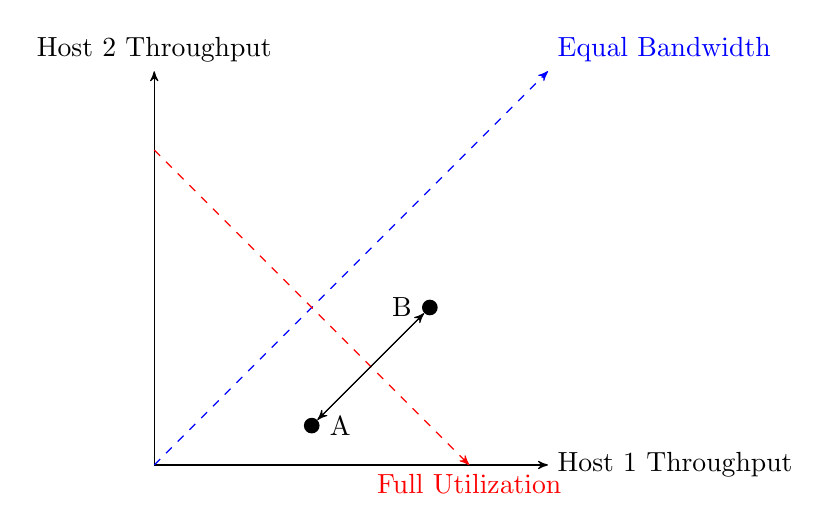
\begin{tikzpicture}[scale=1.0]
        % Axis
        \draw[->] (0,0) -- (5,0) node[right] {Host 1 Throughput};
        \draw[->] (0,0) -- (0,5) node[above] {Host 2 Throughput};
        % Equal Bandwidth Line
        \draw[dashed, blue] (0,0) -- (5,5) node[above right] {Equal Bandwidth};
        % Full Utilization Line
        \draw[dashed, red] (0,4) -- (4,0) node[below] {Full Utilization};
        % Host 1
        \node[label={180:{B}}, circle, fill, inner sep=2pt] (B) at (3.5,2) {};
        % Host 2
        \node[label={0:{A}}, circle, fill, inner sep=2pt] (A) at (2,0.5) {};
        \draw[->] (A) -- (B);
        \draw[->] (B) -- (A);
\end{tikzpicture}


\subsubsection{In Section 3.5.4, we discussed the doubling of the timeout interval after a timeout event. This mechanism is a form of congestion control. Why does TCP need a window-based congestion-control mechanism (as studied in  Section 3.7) in addition to this doubling-timeout-interval mechanism? (P42)}

TCP's use of pipelining allows the sender to have multiple outstanding unacknowledged segments. While a stop-and-wait protocol could rely on doubling the timeout interval as a congestion control mechanism, TCP's pipelining means this approach wouldn't suffice. Even with a doubled timeout interval, TCP can still transmit a large number of packets into a congested network. Thus, a congestion-control mechanism is necessary to manage the flow of data from the application when signs of network congestion arise.



\subsubsection{Host A is sending an enormous file to Host B over a TCP connection. Over this connection there is never any packet loss and the timers never expire. Denote the transmission rate of the link connecting Host A to the Internet by $R$ bps. Suppose that the process in Host A is capable of sending data into its TCP socket at a rate $S$ bps, where $S = 10 \cdot R$. Further suppose that the TCP receive buffer is large enough to hold the entire file, and the send buffer can hold only one percent of the file. What would prevent the process in Host A from continuously passing data to its TCP socket at rate S bps? TCP flow control? TCP congestion control? Or something else? Elaborate. (P43)}

It is not an issue that Host A can send data to its socket 10 times faster than it can transmit it from the socket to the network since the socket is large enough to hold the file. Since the socket of host B can only hold 1 percent of the file, then Host A is limited in its transmission from its socket by how fast host B can read data from its socket. This is controlled by defining the window size of host A tranmissions by TCP congestion control, however since this only limits the transmission from, and not to, host A's socket, there is nothing limiting host A from passing data to its socket at rate $S$.



\subsubsection{Consider sending a large file from a host to another over a TCP connection that has no loss. (P44)}

\textbf{a. Suppose TCP uses AIMD for its congestion control without slow start. Assuming \texttt{cwnd} increases by 1 MSS every time a batch of ACKs is received and assuming approximately constant round-trip times, how long does it take for \texttt{cwnd} increase from 6 MSS to 12 MSS (assuming no loss events)?} \\
No slow start means that \texttt{cwnd} increases by 1 MSS for every RTT. So it will take 6 RTTs for it to increase from 6 MSS to 12 MSS. \\
\\
\textbf{b. What is the average throughput (in terms of MSS and RTT) for this connection up through time = 6 RTT?}
Up to time 6 RTT we have that $1 + 2 + 3 + 4 + 5 + 6 = 21$ MSS have been received. Therefore the throughput up to time 6 RTT is $21/6 = 3.5$ MSS/RTT.



\subsubsection{Consider Figure 3.54. Suppose that at $t_3$, the sending rate at which congestion loss next occurs drops to $0.75 \cdot W_{\max}$ (unbeknownst to the TCP senders, of course). Show the evolution of both TCP Reno and TCP CUBIC for two more rounds each (Hint: note that the times at which TCP Reno and TCP CUBIC react to congestion loss may not be the same anymore). (P45)}

We have that $W_{\max}$ is the congestion window size at which loss last occurred. TCP Reno sets $\texttt{ssthresh} = W_{\max}/2$, sets $\texttt{cwnd} = \texttt{ssthresh} + 3$ MSS (we assume congestion loss is detected by tripple ACK as in figure 3.54) and after quick recovery starts the congestion avoidance phase. Therefore at $t_3 + RTT$ TCP Reno will have set $\texttt{cwnd} = W_{\max}/2 + 3$ and at $t_3 + 2 RTT$ it sets $\texttt{cwnd} = W_{\max}/2 + 4$. \\
\\
TCP Cubic will half the sending rate so that $\texttt{cwnd} =  W_{\max}/2$. TCP Cubic expects loss at time $K$ where $\texttt{cwnd} = 0.75 W_{\max}$ and will set $\texttt{cwnd}_t$ to a cube function of the distance between $t$ and $K$.



\subsubsection{Consider Figure 3.54 again. Suppose that at $t_3$, the sending rate at which congestion loss next occurs increases to $1.5 \cdot Wmax$. Show the evolution of both TCP Reno and TCP CUBIC for at two more rounds each (Hint: see the hint in P45). (P46)}

TCP Reno keep sending in the congestion avoidance phase such that at time $t_3 + RTT$ we have $\texttt{cwnd} = W_{\max}/2 + 1$ and at $t_3 + 2 RTT$ we have $\texttt{cwnd} = W_{\max}/2 + 2$. \\
\\
TCP Cubic expects loss at time $K$ where $\texttt{cwnd} = 1.5 W_{\max}$ and will set $\texttt{cwnd}_t$ to a cube function of the distance between $t$ and $K$.


\subsubsection{Recall the macroscopic description of TCP throughput. In the period of time from when the connection's rate varies from $W/(2 \cdot RTT)$ to $W/RTT$, only one packet is lost (at the very end of the period). (P47)}

\textbf{a. Show that the loss rate (fraction of packets lost) is equal to}
\begin{equation*}
    L = \text{loss rate} = \frac{1}{\frac{3}{8} W^2 + \frac{3}{4}W}
\end{equation*}
\\
The number of packets sent before packet loss, i.e. before $W/(2 \cdot RTT)$ increases to $W/RTT$ can, because of the linear increase in congestion avoidance, be expressed by 
\begin{equation*}
\begin{split}
    \frac{W}{2}+\left(\frac{W}{2}+1\right)+\cdots+W & =\sum_{n=0}^{W / 2}\left(\frac{W}{2}+n\right) \\
    & =\left(\frac{W}{2}+1\right) \frac{W}{2}+\sum_{n=0}^{W / 2} n \\
    & =\left(\frac{W}{2}+1\right) \frac{W}{2}+\frac{W / 2(W / 2+1)}{2} \\
    & =\frac{W^2}{4}+\frac{W}{2}+\frac{W^2}{8}+\frac{W}{4} \\
    & =\frac{3}{8} W^2+\frac{3}{4} W
\end{split}
\end{equation*} 
Since 1 packet is lost every time this amount of packets has been sent we have that the loss rate is
\begin{equation*}
    \frac{1}{\frac{3}{8} W^2+\frac{3}{4} W}
\end{equation*}
\\
\textbf{b. Use the result above to show that if a connection has loss rate $L$, then its average rate is approximately given by}
\begin{equation*}
    \approx \frac{1.22 \cdot MSS}{RTT \sqrt{L}}
\end{equation*}
\\
For large $W$ we have that the quadratic term dominates such that we can approximate the loss rate by 
\begin{equation*}
    L \approx \frac{1}{\frac{3}{8}W^2} = \frac{8}{3W^2}  
\end{equation*}
and express $W$ by 
\begin{equation*}
\begin{split}
    \frac{3L}{8} &\approx \frac{1}{W^2} \\
    W^2 &\approx \frac{8}{3L} \\
    W &\approx \sqrt{\frac{8}{3L}}
\end{split}
\end{equation*}
We have that \cite{kr} states that in exactly these settings we have that the average throughput is $\frac{3}{4}W/RTT$, inserting our value for $W$ (which is in the units of MSS) we get
\begin{equation}
  \label{eq:avg_throughput_with_loss}
    \overline{T} = \frac{\frac{3}{4} \sqrt{\frac{8}{3L}} MSS}{RTT} = \frac{\frac{3}{4} \sqrt{\frac{8}{3}} \frac{1}{\sqrt{L}} MSS}{RTT} = \frac{1.22 MSS}{RTT \sqrt{L}}
\end{equation}



\subsubsection{Consider that only a single TCP (Reno) connection uses one 54 Mbps wireless link which does not buffer any data. Suppose that this link is the only congested link between the sending and receiving hosts. Assume that the TCP sender has a huge file to send to the receiver and the receiver's receive buffer is much larger than the congestion window. We also make the following assumptions: each TCP segment size is 536 bytes; the two-way propagation delay of this connection is 6 msec; and this TCP connection is always in congestion avoidance phase, that is, ignore slow start. (P48)}

\textbf{a. What is the maximum window size (in segments) that this TCP connection can achieve?} \\
Since the receiver buffer is larger than the congestion window then packet loss can only occur in the link, which happens as soon as queuing occurs since it does not buffer. Therefore the maximum window size must be set so the hosts do not send faster than the link's capacity. \\
\\
Sending at link capacity will mean that 
\begin{equation*}
\begin{split}
    \frac{W \cdot MSS}{RTT} &= 54 \, \text{Mbps} \\
    W &= \frac{RTT}{MSS} 54 \, \text{Mbps}
\end{split}
\end{equation*}
We have that $MSS = 536 \cdot 8$ bits and assuming negligible processing- and queuing delay we hat have that $RTT = 12 \cdot 10^{-3}$ seconds, which is the two times the two-way propagation delay (one for each side of the link). Inserting these values we can determine $W$ by
\begin{equation*}
\begin{split}
    W &= \frac{12 \cdot 10^{-3} \, \text{s}}{536 \cdot 8 \, \text{bits}} 54 \cdot 10^6 \, \text{bits/s} \\
    &= 151.12
\end{split}
\end{equation*}
Flooring this value to make in an integer that does not go over the link capacity results in a maximum window size of $W = 151$ MSS. \\
\\
\textbf{b. What is the average window size (in segments) and average throughput (in bps) of this TCP connection?} \\
We have that the window will vary from $W/2$ (which is set on loss and increase linearly) to $W$. The average window size is therefore 
\begin{equation*}
    \overline{W} = \frac{W/2 + W}{2} = \frac{W}{4} + \frac{W}{2} = \frac{3}{4} W = \frac{3}{4} 151 = 113.25
\end{equation*}
\\
The average throughput $\overline{T}$ can be expressed by
\begin{equation*}
    \overline{T} = \frac{\overline{W} \cdot MSS}{RTT} = \frac{113.25 \cdot 536 \cdot 8 \, \text{bits}}{12 \cdot 10^{-3} \, \text{s}} = 40.468 \cdot 10^6 \, \text{bits/s}
\end{equation*}
\\
\textbf{c. How long would it take for this TCP connection to reach its maximum window again after recovering from a packet loss?} \\
This is equivalent to the time it takes to increase the window size from $W/2$ to $W$ which can be expressed as
\begin{equation*}
    \lr{W - W/2} RTT = W/2 \cdot RTT  = \frac{151}{2} \cdot 12 \cdot 10^{-3} \, \text{s} = 0.906 \, \text{s}
\end{equation*}
since the window size increases by 1 MSS every RTT.

\subsubsection{Consider the scenario described in the previous problem. Suppose that the 10 Mbps link can buffer a finite number of segments. Argue that in order for the link to always be busy sending data, we would like to choose a buffer size that is at least the product of the link speed C and the two-way propagation delay between the sender and the receiver. (P49)}

In TCP's sliding window protocol, multiple segments can be transmitted before receiving acknowledgements. During the round-trip time $RTT$, the sender can transmit up to $C \times RTT$ bits of data while waiting for acknowledgements from previously sent segments. \\
\\
If the buffer size is less than $C \times RTT$, then after transmitting all buffered data, the sender must wait for acknowledgements before it can send more data, which creates idle time on the link. However, if the buffer size is at least $C \times RTT$, there will always be sufficient data available to transmit during the acknowledgement delay period, which ensures the link remains continuously busy.\\
\\
Therefore, the minimum buffer size required is:
$$\text{Buffer size} \geq C \times RTT$$

\subsubsection{Repeat Problem 48, but replacing the 54 Mbps link with a 100 Gbps link and an RTT of 60 ms. Note that in your answer to part c, you will realize that it takes a very long time for the congestion window size to reach its maximum window size after recovering from a packet loss. Can you consider solutions for this? (P50)}

\textbf{a. What is the maximum window size (in segments) that this TCP connection can achieve?} \\
As before we have that since the receiver buffer is larger than the congestion window then packet loss can only occur in the link, which happens as soon as queuing occurs since it does not buffer. Therefore the maximum window size must be set so the hosts do not send faster than the link's capacity. \\
\\
Sending at link capacity will mean that 
\begin{equation*}
\begin{split}
    \frac{W \cdot MSS}{RTT} &= 100 \, \text{Gbps} \\
    W &= \frac{RTT}{MSS} 100 \, \text{Gbps}
\end{split}
\end{equation*}
We have that $MSS = 536 \cdot 8$ bits and assuming negligible processing- and queuing delay we hat have that $RTT = 120 \cdot 10^{-3}$ seconds, which is the two times the two-way propagation delay (one for each side of the link). Inserting these values we can determine $W$ by
\begin{equation*}
\begin{split}
    W &= \frac{120 \cdot 10^{-3} \, \text{s}}{536 \cdot 8 \, \text{bits}} 100 \cdot 10^9 \, \text{bits/s} \\
    &= 2798507.46
\end{split}
\end{equation*}
Flooring this value to make in an integer that does not go over the link capacity results in a maximum window size of $W = 2798507$ MSS. \\
\\
\textbf{b. What is the average window size (in segments) and average throughput (in bps) of this TCP connection?} \\
We have that the window will vary from $W/2$ (which is set on loss and increase linearly) to $W$. The average window size is therefore 
\begin{equation*}
    \overline{W} = \frac{W/2 + W}{2} = \frac{W}{4} + \frac{W}{2} = \frac{3}{4} W = \frac{3}{4} 2798507 = 2098880.25
\end{equation*}
\\
The average throughput $\overline{T}$ will can be expressed by
\begin{equation*}
    \overline{T} = \frac{\overline{W} \cdot MSS}{RTT} = \frac{2098880.25 \cdot 536 \cdot 8 \, \text{bits}}{120 \cdot 10^{-3} \, \text{s}} = 74999.9876 \cdot 10^6 \, \text{bits/s}
\end{equation*}
\\
\textbf{c. How long would it take for this TCP connection to reach its maximum window again after recovering from a packet loss?} \\
This is equivalent to the time it takes to increase the window size from $W/2$ to $W$ which can be expressed as
\begin{equation*}
    \lr{W - W/2} RTT = W/2 \cdot RTT  = \frac{2798507}{2} \cdot 120 \cdot 10^{-3} \, \text{s} = 167910.42 \, \text{s}
\end{equation*}
since the window size increases by 1 MSS every RTT. As the problem description states, this is indeed a long time. A solution could be to use TCP Cubic instead.


\subsubsection{Let $T$ (measured by RTT) denote the time interval that a TCP connection takes to increase its congestion window size from $W/2$ to $W$, where $W$ is the maximum congestion window size. Argue that $T$ is a function of TCP's average throughput. (P51)}

From equation \ref{eq:avg_throughput_with_loss} we have that
\begin{equation*}
  \begin{split}
    \overline{T} &= \frac{1.22 \cdot MSS}{RTT \sqrt{L}} \Longleftrightarrow \\
    \overline{T} \cdot RTT \cdot \sqrt{L} &= 1.22 \cdot MSS \Longleftrightarrow \\
    \sqrt{L} &= \frac{1.22 \cdot MSS}{\overline{T} \cdot RTT} \Longleftrightarrow \\
    L &= \lr{\frac{1.22 \cdot MSS}{\overline{T} \cdot RTT}}^2
  \end{split}
\end{equation*}
with $L$ being the loss rate, i.e. lost packet per packets sent. Therefore we must have that on average we send $1/L$ packets between two consecutive packet losses. We have that on average we send $MSS/\overline{T}$ packets per RTT, and increase the windows size by 1 MSS for each packet sent without packet loss. We must therefore have that the time in RTT it takes for the window size to double is expected to be
\begin{equation*}
  T = 1/L \cdot \frac{MSS}{\overline{T}}  
\end{equation*}
Inserting $L$ we get
\begin{equation*}
  \begin{split}
    T &= \frac{1}{ \lr{\frac{1.22 \cdot MSS}{\overline{T} \cdot RTT}}^2} \frac{MSS}{\overline{T}}  \\
    &= \frac{\overline{T}^2 \cdot RTT^2}{1.22^2 \cdot MSS^2} \frac{MSS}{\overline{T}} \\
    &= \frac{RTT^2 \cdot \overline{T}}{1.22^2 \cdot MSS}
  \end{split}
\end{equation*}
which shows $T$ as a function of average throughput $\overline{T}$ for TCP (Reno).


\subsubsection{Consider a simplified TCP's AIMD algorithm where the congestion window size is measured in number of segments, not in bytes. In additive increase, the congestion window size increases by one segment in each RTT. In multiplicative decrease, the congestion window size decreases by half (if the result is not an integer, round down to the nearest integer). Suppose that two TCP connections, C1 and C2, share a single congested link of speed 30 segments per second. Assume that both C1 and C2 are in the congestion avoidance phase. Connection C1's RTT is 50 msec and connection C2's RTT is 100 msec. Assume that when the data rate in the link exceeds the link's speed, all  TCP connections experience data segment loss. (P52)}

\textbf{a. If both $C_1$ and $C_2$ at time $t_0$ have a congestion window of 10 segments, what are their congestion window sizes after 1000 msec?} \\
The congestion window will increase with one segment per received ACK, which for C1 is every 50 msec and for C2 every 100 msec. When the sum of window sizes exceeds 30 both connections will experience a loss after RTT where they will halve their window sizes. This means that the window size will follow the development shown in table below where it is shown in red when the sum of segments on the link exceeds 30. \\
\begin{center}
\begin{tabular}{ccc}
  \hline
  Time (msec) & C1 window size (segments) & C2 window size (segments) \\
  \hline
  0 & 10 & 10 \\
  50 & 11 & 10 \\
  100 & 12 & 11 \\
  150 & 13 & 11 \\
  200 & 14 & 12 \\
  250 & 15 & 12 \\
  300 & 16 & 13 \\
  350 & 17 & 13 \\
  400 & \textcolor{red}{18} & \textcolor{red}{14} \\
  450 & 9 & 14 \\
  500 & 10 & 7 \\
  550 & 11 & 7 \\
  600 & 12 & 8 \\
  650 & 13 & 8 \\
  700 & 14 & 9 \\
  750 & 15 & 9 \\
  800 & 16 & 10 \\
  850 & 17 & 10 \\
  900 & 18 & 11 \\
  950 & 19 & 11 \\
  1000 & \textcolor{red}{20} & \textcolor{red}{12} \\
  \hline
\end{tabular}
\end{center}
Here we see that the window sizes at 1000 msec is 20 for C1 and 12 for C2. Even though the link speed is exceeded at this time none of them have yet experienced that a loss have happened. \\
\\
\textbf{b. In the long run, will these two connections get the same share of the band-width of the congested link? Explain.} \\
No, as seen in the table of part a, C1 will have a head start on C2 since it will increase its window size faster and thus have the largest size when a loss occur for which both connections will half their sizes, and C1 have the largest window size after the halving. C1 will after this loss again increase faster and have an even larger proportion of the the bandwidth when a loss again occurs. In this way C2 will increase its share of the bandwidth until an equilibrium is reached from which C1 can never hope to reach half of the bandwidth.


\subsubsection{Consider the network described in the previous problem. Now suppose that the two TCP connections, C1 and C2, have the same RTT of 100 msec.  Suppose that at time $t_0$, C1's congestion window size is 15 segments but C2's congestion window size is 10 segments. (P53)}

\textbf{a. What are their congestion window sizes after 2200 msec?} \\
Both C1 and C2 will increase their window sizes with 1 segment every 100 msec and will both halve the window size when the sum of window sizes exceeds 30 segments. Both connections will know a loss occurred 100 msec after. This means that the development of the window sizes of C1 and C2 can be shown as the table below.
\begin{center}
  \begin{tabular}{ccc}
    \hline
    Time (msec) & C1 window size (segments) & C2 window size (segments) \\
    \hline
    0 & 15 & 10 \\
    100 & 16 & 11 \\
    200 & 17 & 12 \\
    300 & \textcolor{red}{18} & \textcolor{red}{13} \\
    400 & 7 & 6 \\
    500 & 8 & 7 \\
    600 & 9 & 8 \\
    700 & 10 & 9 \\
    800 & 11 & 10 \\
    900 & 12 & 11 \\
    1000 & 13 & 12 \\
    1100 & 14 & 13 \\
    1200 & 15 & 14 \\
    1300 & \textcolor{red}{16} & \textcolor{red}{15} \\
    1400 & 8 & 7 \\
    1500 & 9 & 8 \\
    1600 & 10 & 9 \\
    1700 & 11 & 10 \\
    1800 & 12 & 11 \\
    1900 & 13 & 12 \\
    2000 & 14 & 13 \\
    2100 & 15 & 14 \\
    2200 & \textcolor{red}{16} & \textcolor{red}{15} \\
    \hline
  \end{tabular}
\end{center}
Where we see that the window size at 2200 msec is 16 for C1 and 15 for C2. \\
\\
\textbf{b. In the long run, will these two connections get about the same share of the bandwidth of the congested link?} \\
Close to equal share but never exact. We can see this from the table in part a, where there is an infinite pattern in how the connections experience loss when C1 has window size 16 and C2 15. This occurs because we round down, which makes C1 have size 8 and C2 size 7 after a loss. Since they both increase at the same rate C2 will never catch up to C1 (which it could have we decided to round up to nearest integer when halving the window size). \\
\\
\textbf{c. We say that two connections are synchronized, if both connections reach their maximum window sizes at the same time and reach their minimum window sizes at the same time. In the long run, will these two connections get synchronized eventually? If so, what are their maximum window sizes?} \\
No, they are not. As argued in part b there is an infinite pattern in which, after 1300 msec the window size of C1 is never increased above 16 and the window size of C2 is never increased above 15. C1 reaches its max at 300 msec with a size of 18, but C2 reaches its max at 1300 msec and every 900 msec with a size of 15.\\
\\
\textbf{d. Will this synchronization help to improve the utilization of the shared link? Why? Sketch some idea to break this synchronization.} \\
No. These connections oscillate between a lower and higher window size just like a single connection would. The link is therefore not utilised after a loss. A way to improve this and break synchronisation would be to add a finite buffer to the link that prior to buffer overflow randomly drops packets. This would add asynchronous handling of loss in the connection even though they increase their window size at the same rate, which in turn will make it possible for one connection to keep increasing their window size (this utilising the link) when another has halved its window size after experiencing loss.


\subsubsection{Consider a modification to TCP's congestion control algorithm. Instead of additive increase, we can use multiplicative increase. A TCP sender increases its window size by a small positive constant a (0 < a < 1) whenever it receives a valid ACK. Find the functional relationship between loss rate L and maximum congestion window $W$. Argue that for this modified TCP, regardless of TCP's average throughput, a TCP connection always spends the same amount of time to increase its congestion window size from $W/2$ to $W$. (P54)}


\subsubsection{In our discussion of TCP futures in Section 3.7, we noted that to achieve a throughput of 10 Gbps, TCP could only tolerate a segment loss probability of $2 \cdot 10^{-10}$ (or equivalently, one loss event for every 5,000,000,000 segments). Show the derivation for the values of $2 \cdot 10^{-10}$ (1 out of 5,000,000) for the RTT and MSS values given in Section 3.7. If TCP needed to support a  100 Gbps connection, what would the tolerable loss be? (P55)}


\subsubsection{In our discussion of TCP congestion control in Section 3.7, we implicitly assumed that the TCP sender always had data to send. Consider now the case that the TCP sender sends a large amount of data and then goes idle (since it has no more data to send) at $t_1$. TCP remains idle for a relatively long period of time and then wants to send more data at $t_2$. What are the advantages and disadvantages of having TCP use the cwnd and ssthresh values from t1when starting to send data at $t_2$? What alternative would you recommend? Why? (P56)}


\subsubsection{In this problem, we investigate whether either UDP or TCP provides a degree of end-point authentication. (P57)}

\textbf{a. Consider a server that receives a request within a UDP packet and responds to that request within a UDP packet (for example, as done by a DNS server). If a client with IP address X spoofs its address with address Y, where will the server send its response?} \\
The server uses the source IP address in the received UDP packet to determine where to send the response. Since the packet appears to come from address Y, the server will send its response to the spoofed address Y. \\
\\
\textbf{b. Suppose a server receives a SYN with IP source address Y, and after responding with a SYNACK, receives an ACK with IP source address Y with the correct acknowledgment number. Assuming the server chooses a random initial sequence number and there is no ''man-in-the-middle,'' can the server be certain that the client is indeed at Y (and not at some other address X that is spoofing Y)?} \\
If someone was spoofind the Y address then they would not receive the SYNACK, which was sent to address Y along with the random sequence number. This means that the host at address Y would not send back an ACK since this host has not initialzed a three-way-handshake with SYN. If the spoofer were able to appropriately time an ACK to the server then they would still not be able to know the random sequence number (since we assume no man-in-the-middle to intecept this number). Therefore receiving an ACK with the correct sequence number ensures that the server can be certain that the client is indeed Y, so the answer is yes.

\subsubsection{In this problem, we consider the delay introduced by the TCP slow-start phase. Consider a client and a Web server directly connected by one link of rate $R$. Suppose the client wants to retrieve an object whose size is exactly equal to 15 $S$, where $S$ is the maximum segment size (MSS). Denote the round-trip time between client and server as RTT (assumed to be constant). Ignoring protocol headers, determine the time to retrieve the object (including TCP connection establishment) when: (P58)}

\textbf{a. $4 S/R > S/R + RTT > 2 S/R$} \\
\\
\textbf{b. $S/R + RTT > 4 S/R$} \\
\\
\textbf{c. $S/R > RTT$} \\

%%% Local Variables:
%%% mode: LaTeX
%%% TeX-master: "../../kr"
%%% End:

\subsection{Programming Assignments}

\section{The Network Layer: Data Plane}
\subsection{Overview of Network Layer}


\subsection{What's Inside a Router?}
\subsection{The Internet Protocol (IP): IPv4, Addressing, IPv6, and More}
\subsection{Generalized Forwarding and SDN}
\subsection{Middleboxes}
\subsection{Problems}

\bibliographystyle{agsm}
\nocite{*}
\bibliography{bibFile} 
\end{document}